% Лабораторная работа по РЗП № 1
% Дуников Константин Артёмович

% Тип документа: статья, на бумаге А4
\documentclass[a4paper]{article}

% Подключение сторонних tex файлов 
\usepackage{import}


% Основные данные - ВУЗ, факультет, город...
\import{./../../../stuff/tex}{config.tex}

% Подключение необходимых зависимостей
\import{./../../../stuff/tex/settings}{packages.tex}
% Настройка подключенных пакетов
\import{./../../../stuff/tex/settings}{preferences.tex}


% Шаблон титульной страницы 
\import{./../../../stuff/tex/templates}{title.tex}
% Упрощенный блок "выполнил"
\import{./../../../stuff/tex/templates}{sign1.tex}
% Макрос для содержания
\import{./../../../stuff/tex/templates}{toc.tex}

% Определяем название документа
\title{
  Лабораторная работа №1 по курсу \\
  <<Разработка защищенных приложений>> \\
  Атака CSRF
}
% Отключаем отображение правительства
\renewcommand{\government}{}
% Отключаем сокращенное нзавание университета
\renewcommand{\subuniversity}{}
% Указываем преподавателя
\renewcommand{\shortteachername}{Башун В.В.}


% Путь до внешних изображений
\graphicspath{ {./../figures/csfr}}


% Основной текст работы
\begin{document}
  \templatedtitlepage
  
  \toc
  \section{Ход работы}

  \subsection{Подготовка. Запуск ВМ}

  \begin{figure}[H]
    \centering
    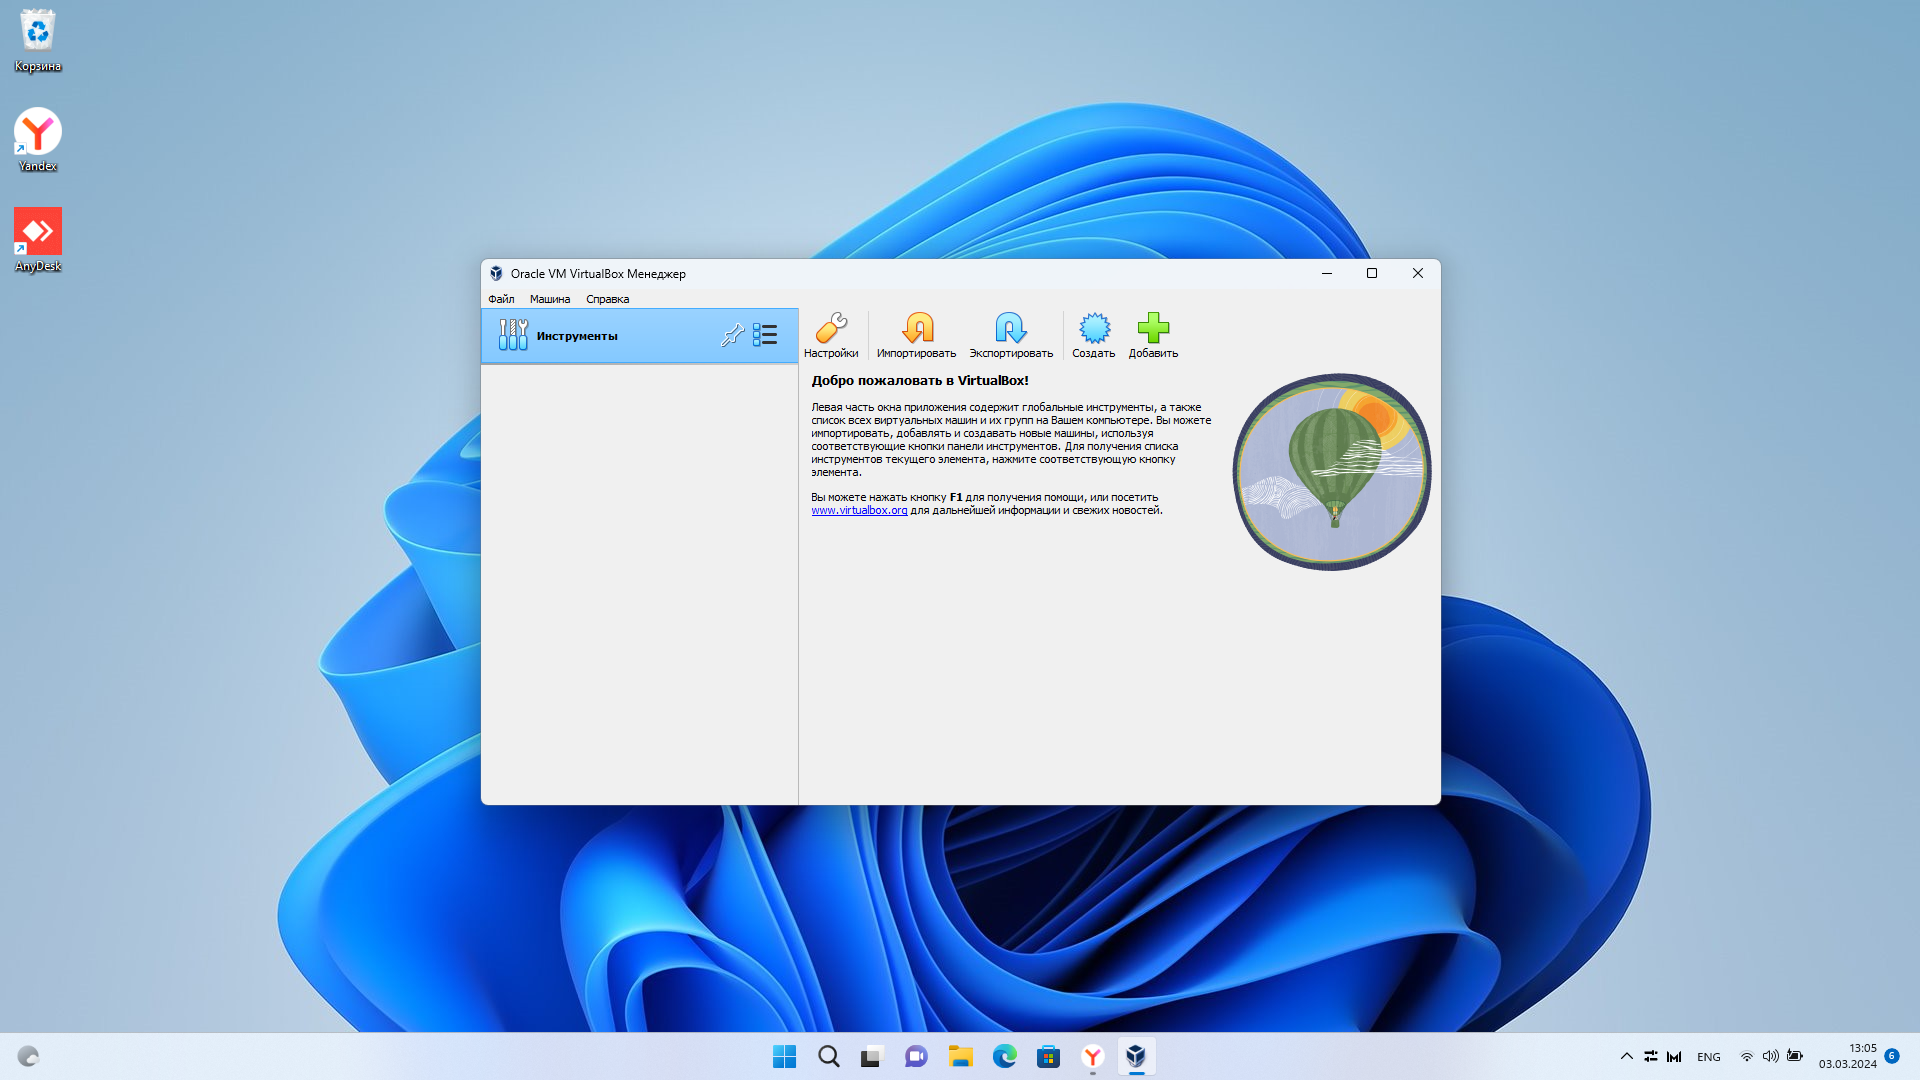
\includegraphics[width=\textwidth]{Screenshot_2}
    \caption{Открываем Virtual Box}
  \end{figure}

  \begin{figure}[H]
    \centering
    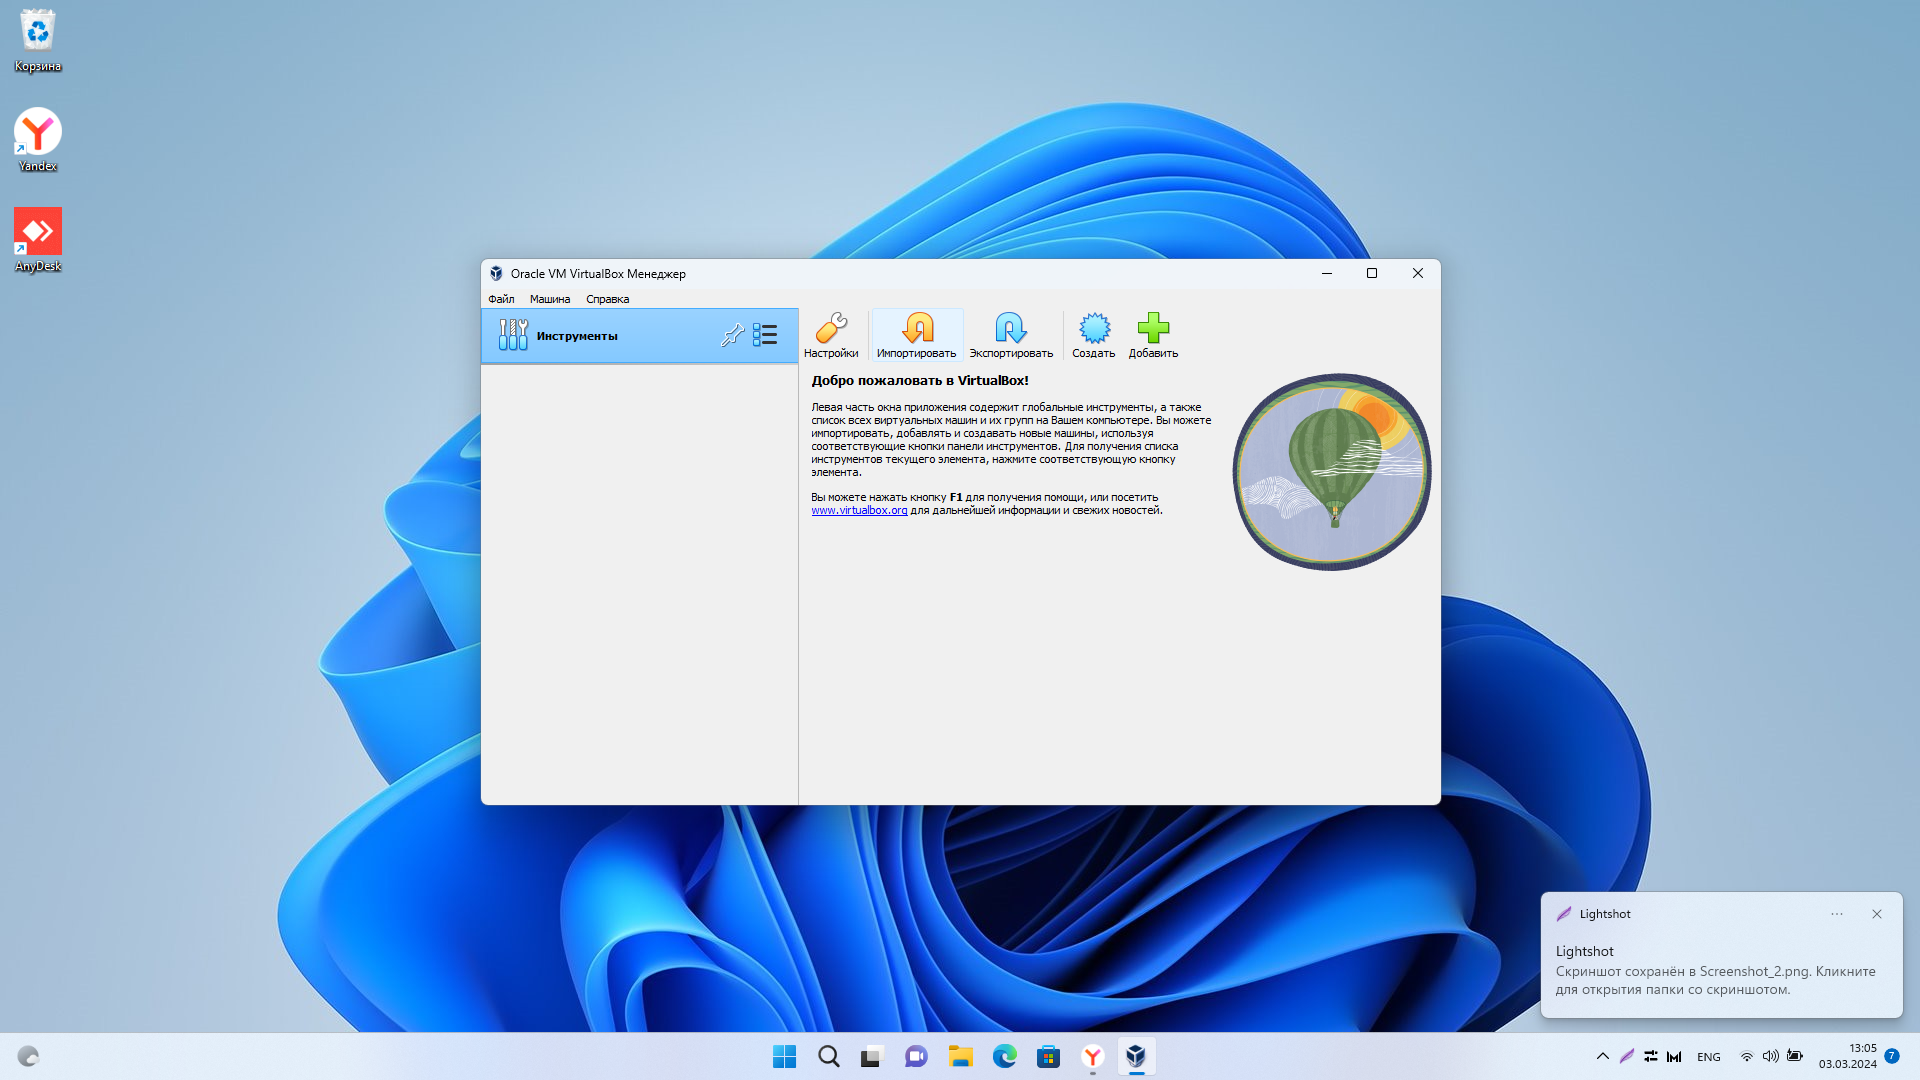
\includegraphics[width=\textwidth]{Screenshot_3}
    \caption{Запускаем импорт уже готовой виртуальной машине}
  \end{figure}

  \begin{figure}[H]
    \centering
    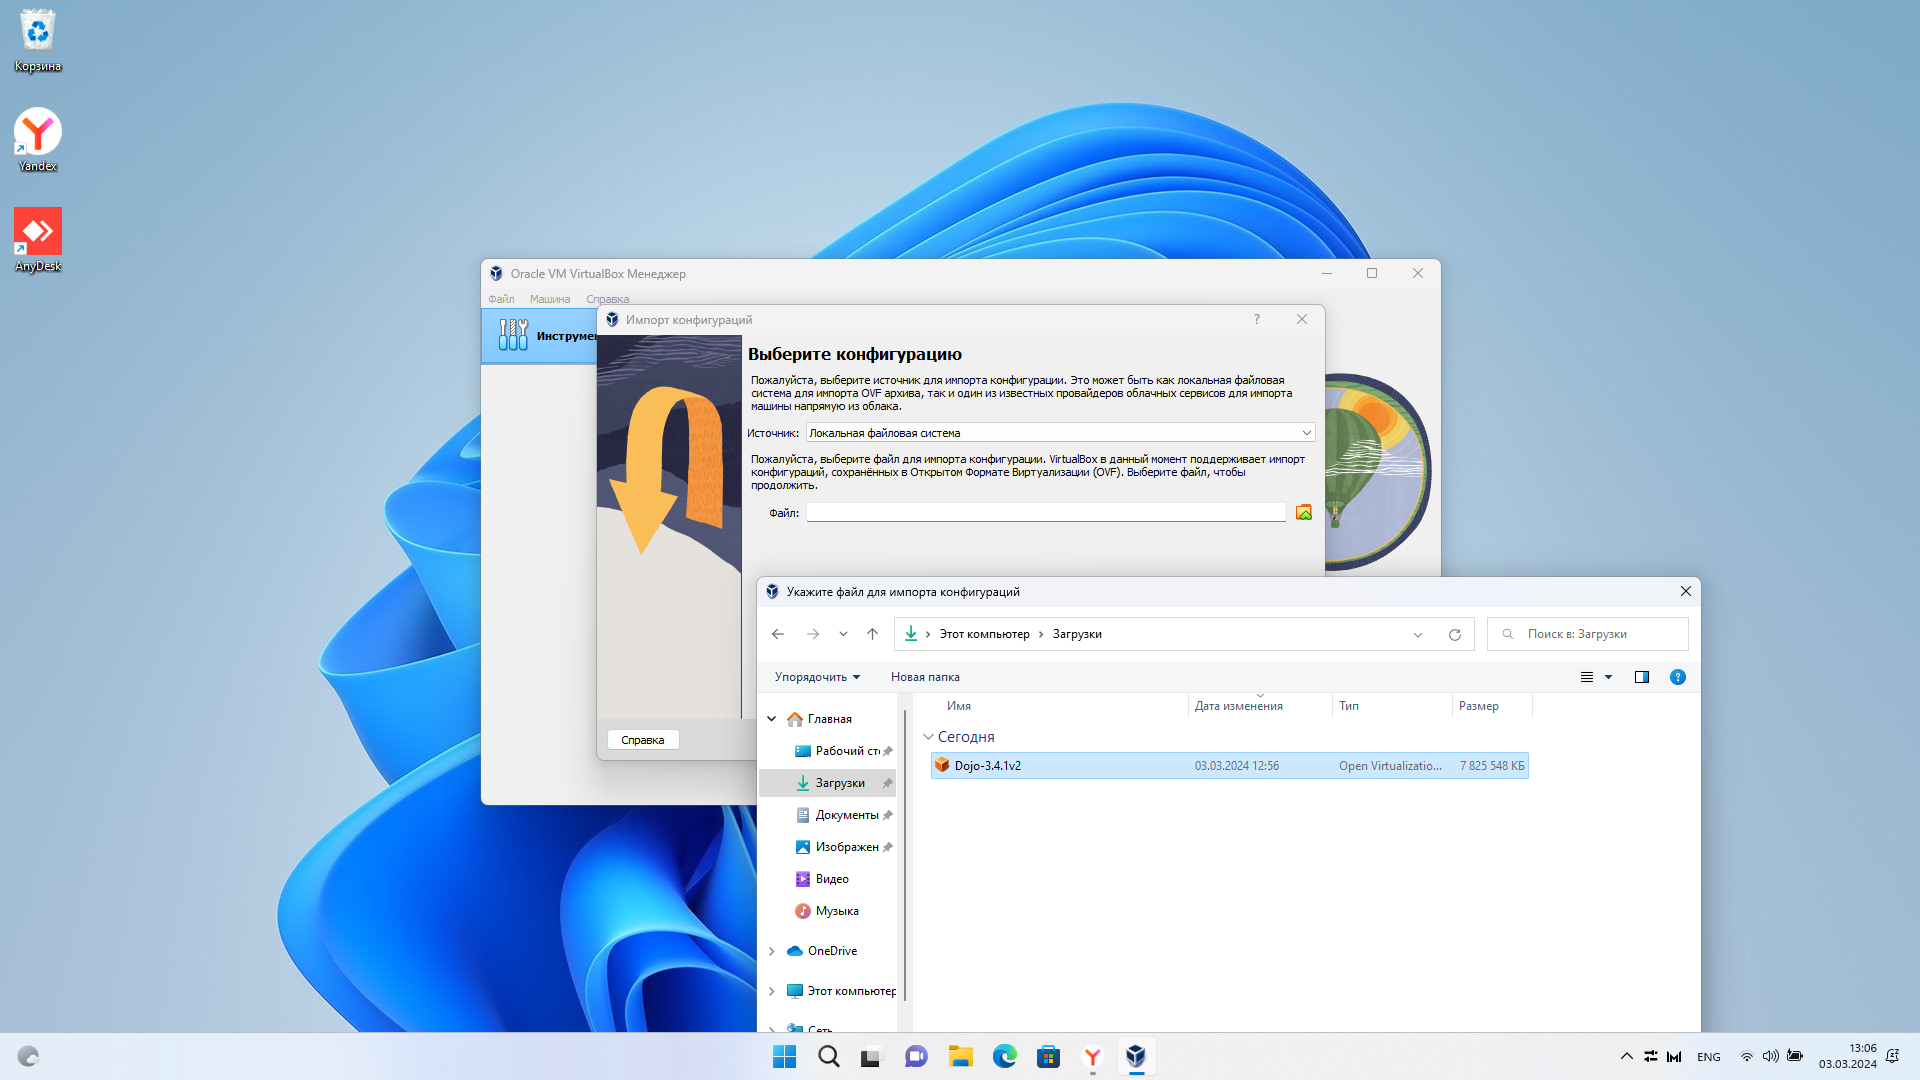
\includegraphics[width=\textwidth]{Screenshot_4}
    \caption{Указываем путь к необходимому образу}
  \end{figure}

  \begin{figure}[H]
    \centering
    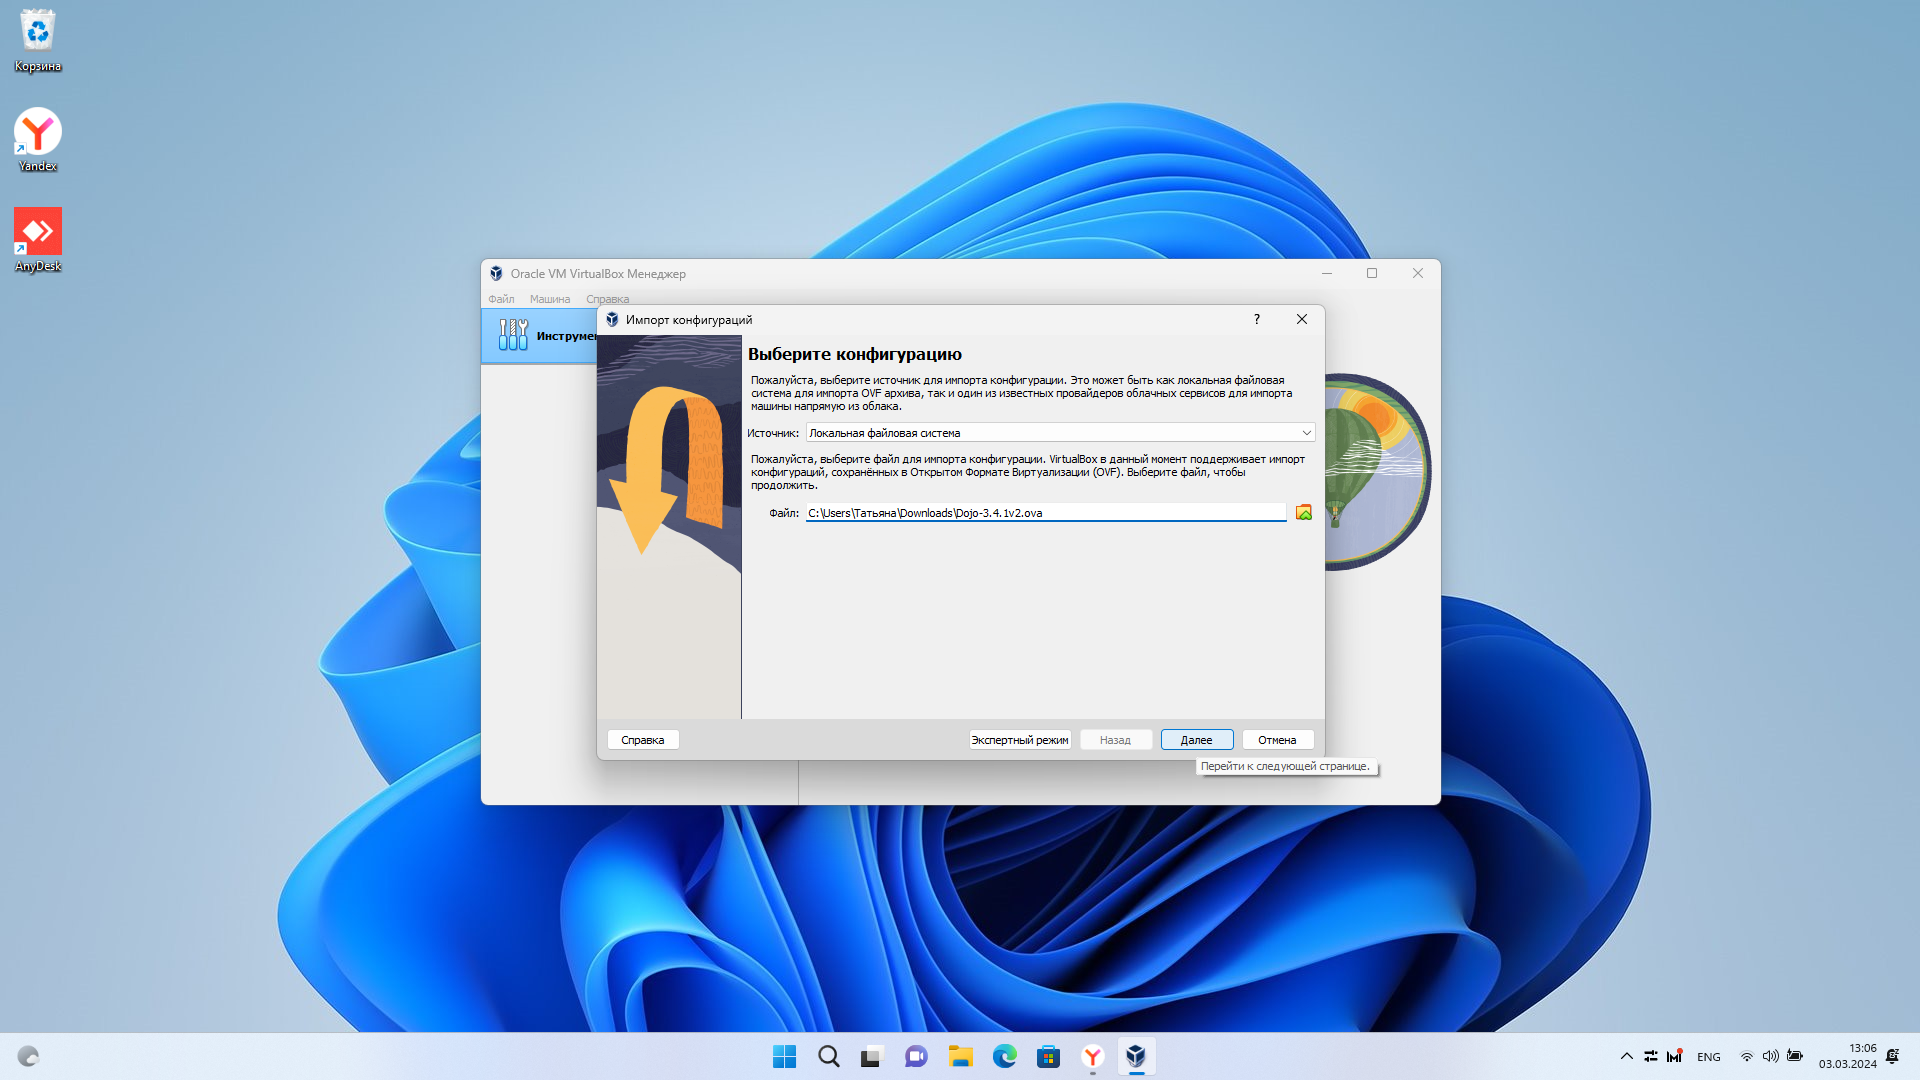
\includegraphics[width=\textwidth]{Screenshot_5}
    \caption{Далее}
  \end{figure}

  \begin{figure}[H]
    \centering
    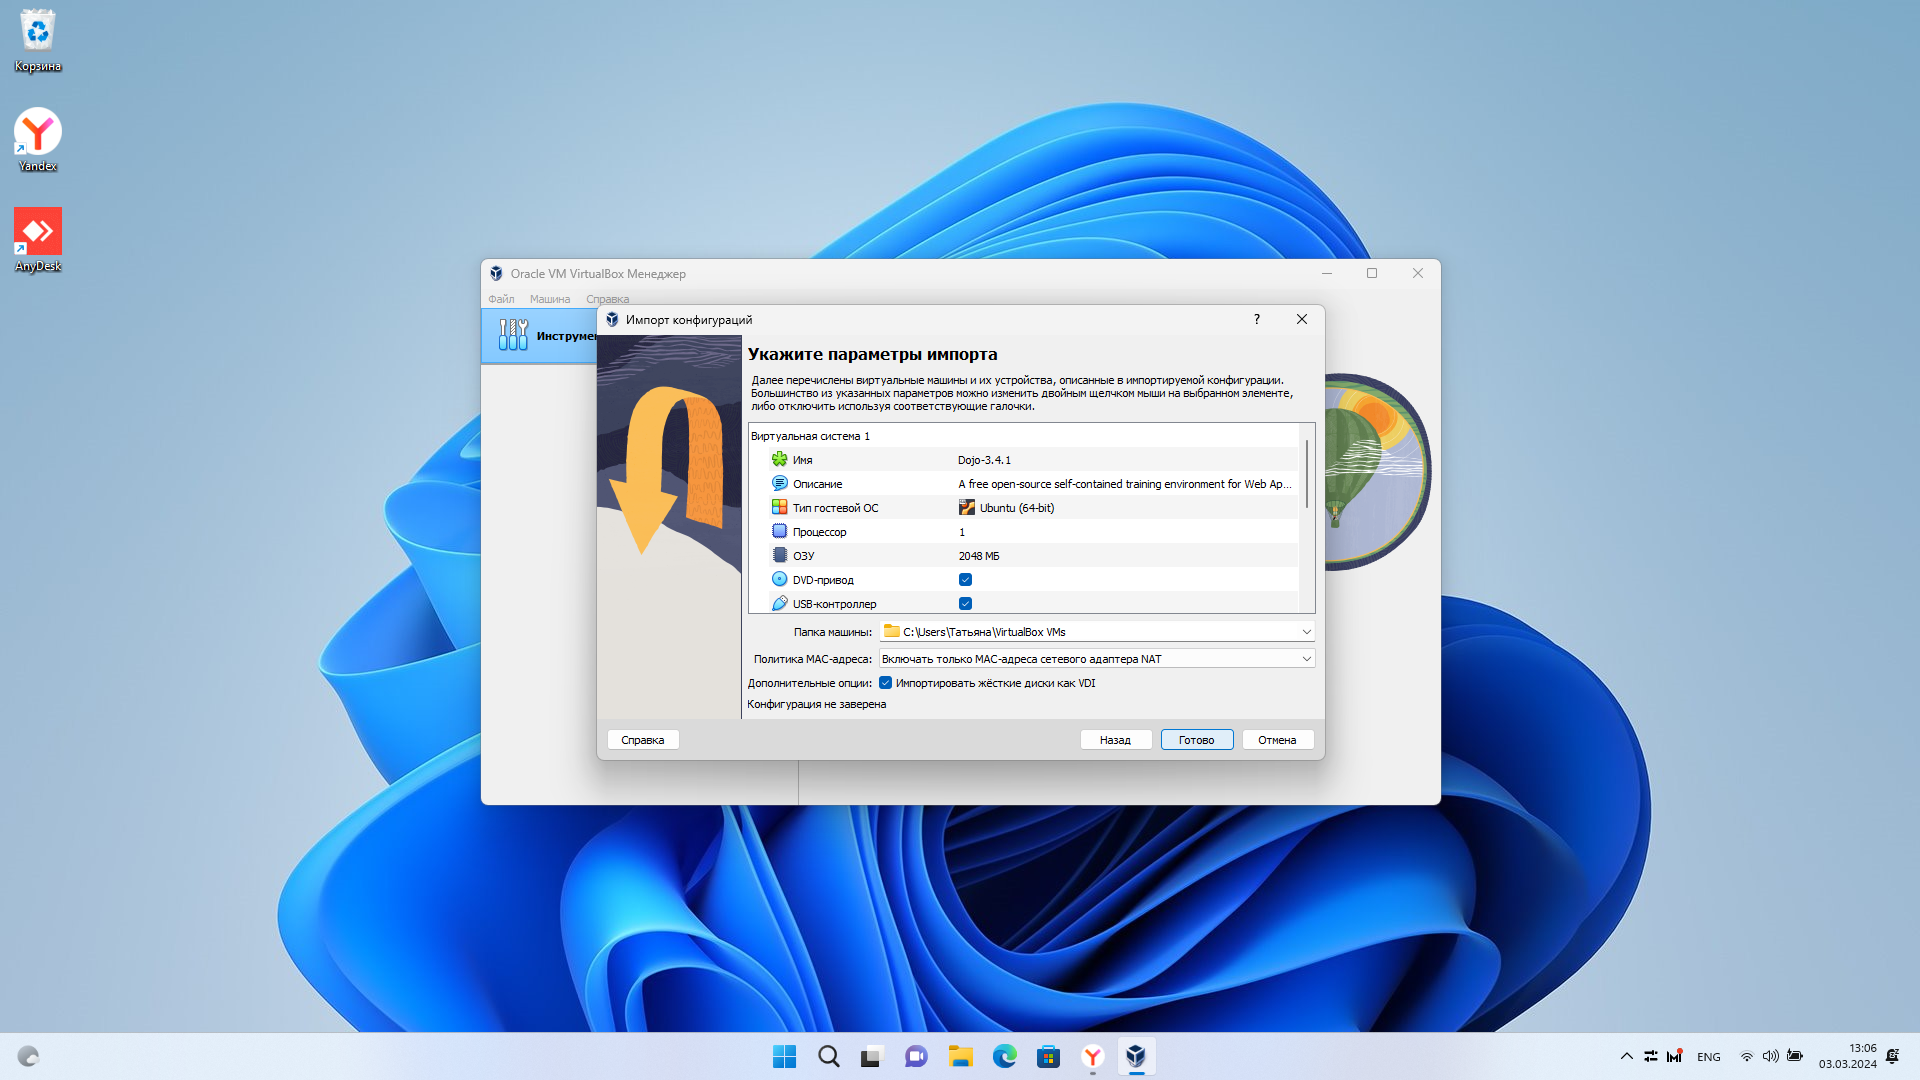
\includegraphics[width=\textwidth]{Screenshot_6}
    \caption{Все параметры машины оставляем по умолчанию}
  \end{figure}

  \begin{figure}[H]
    \centering
    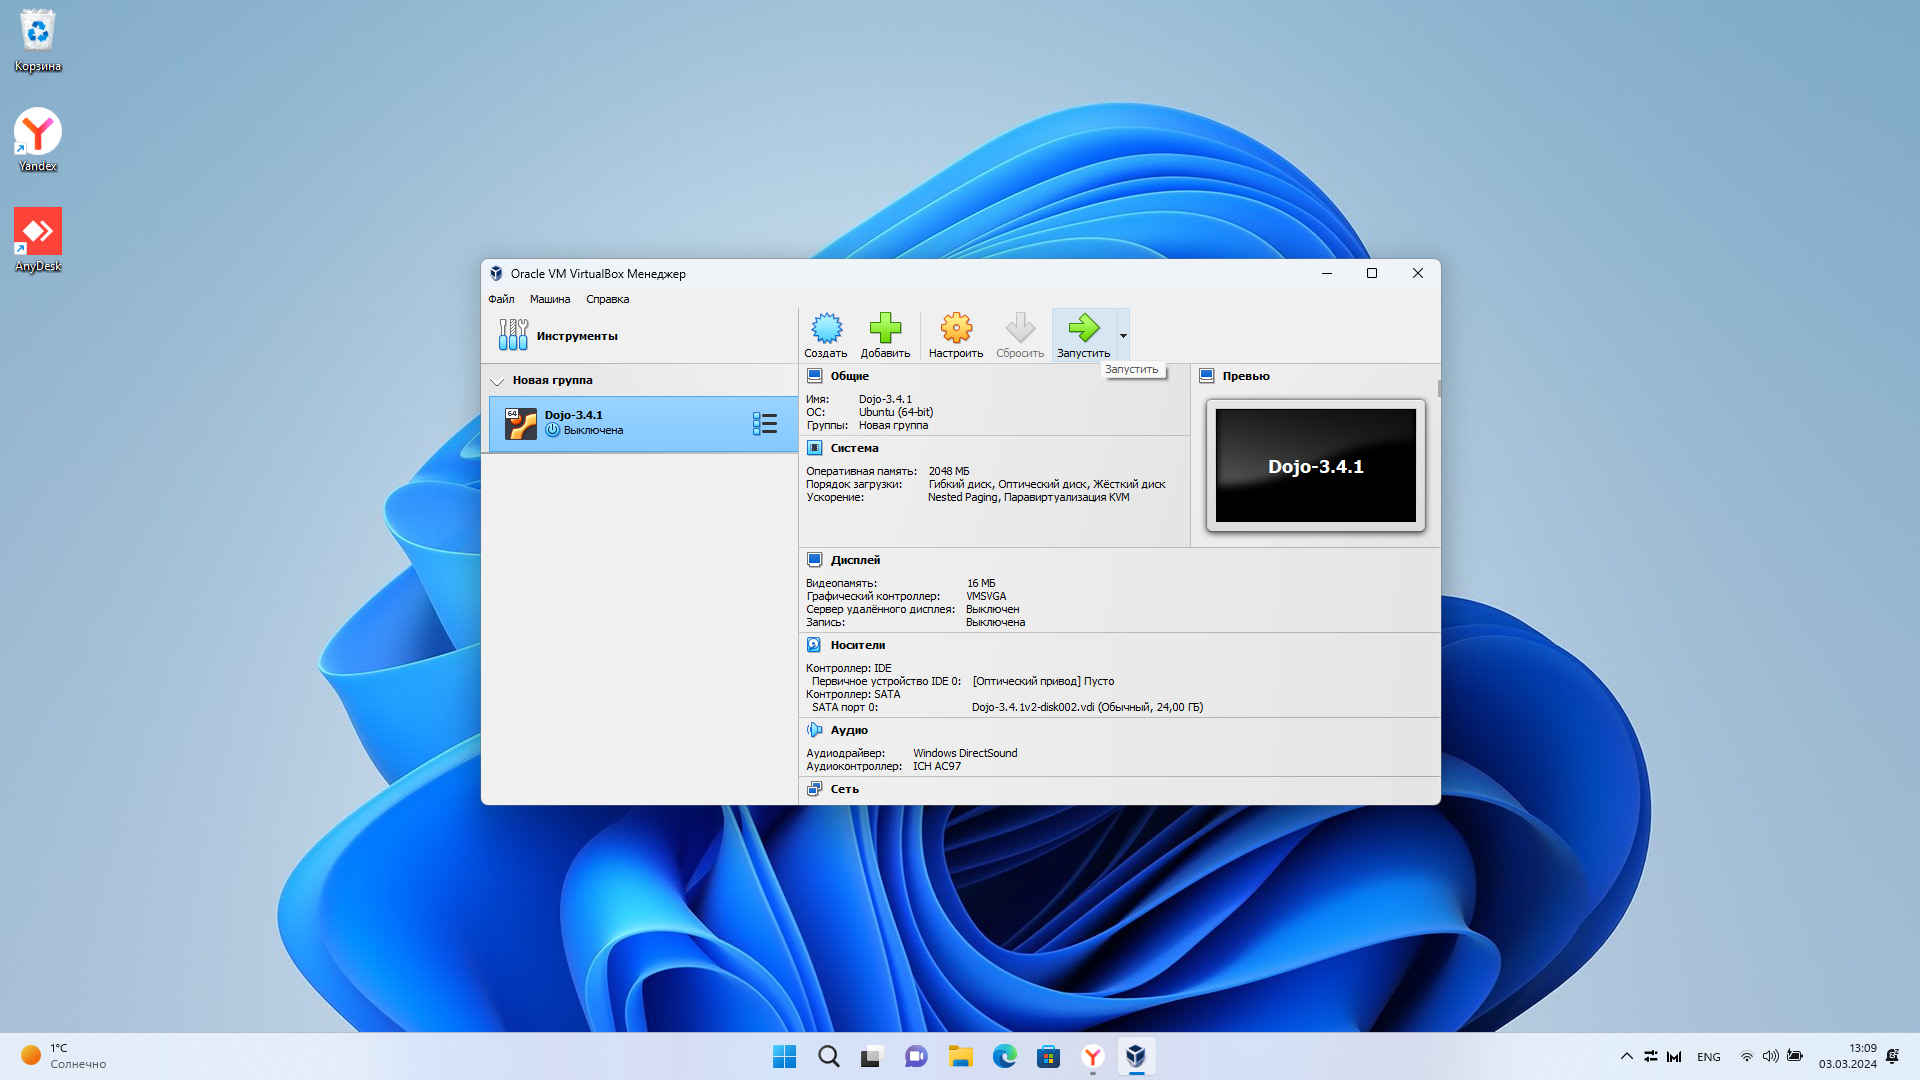
\includegraphics[width=\textwidth]{Screenshot_7}
    \caption{Виртуальная машина готова к работе}
  \end{figure}

  \begin{figure}[H]
    \centering
    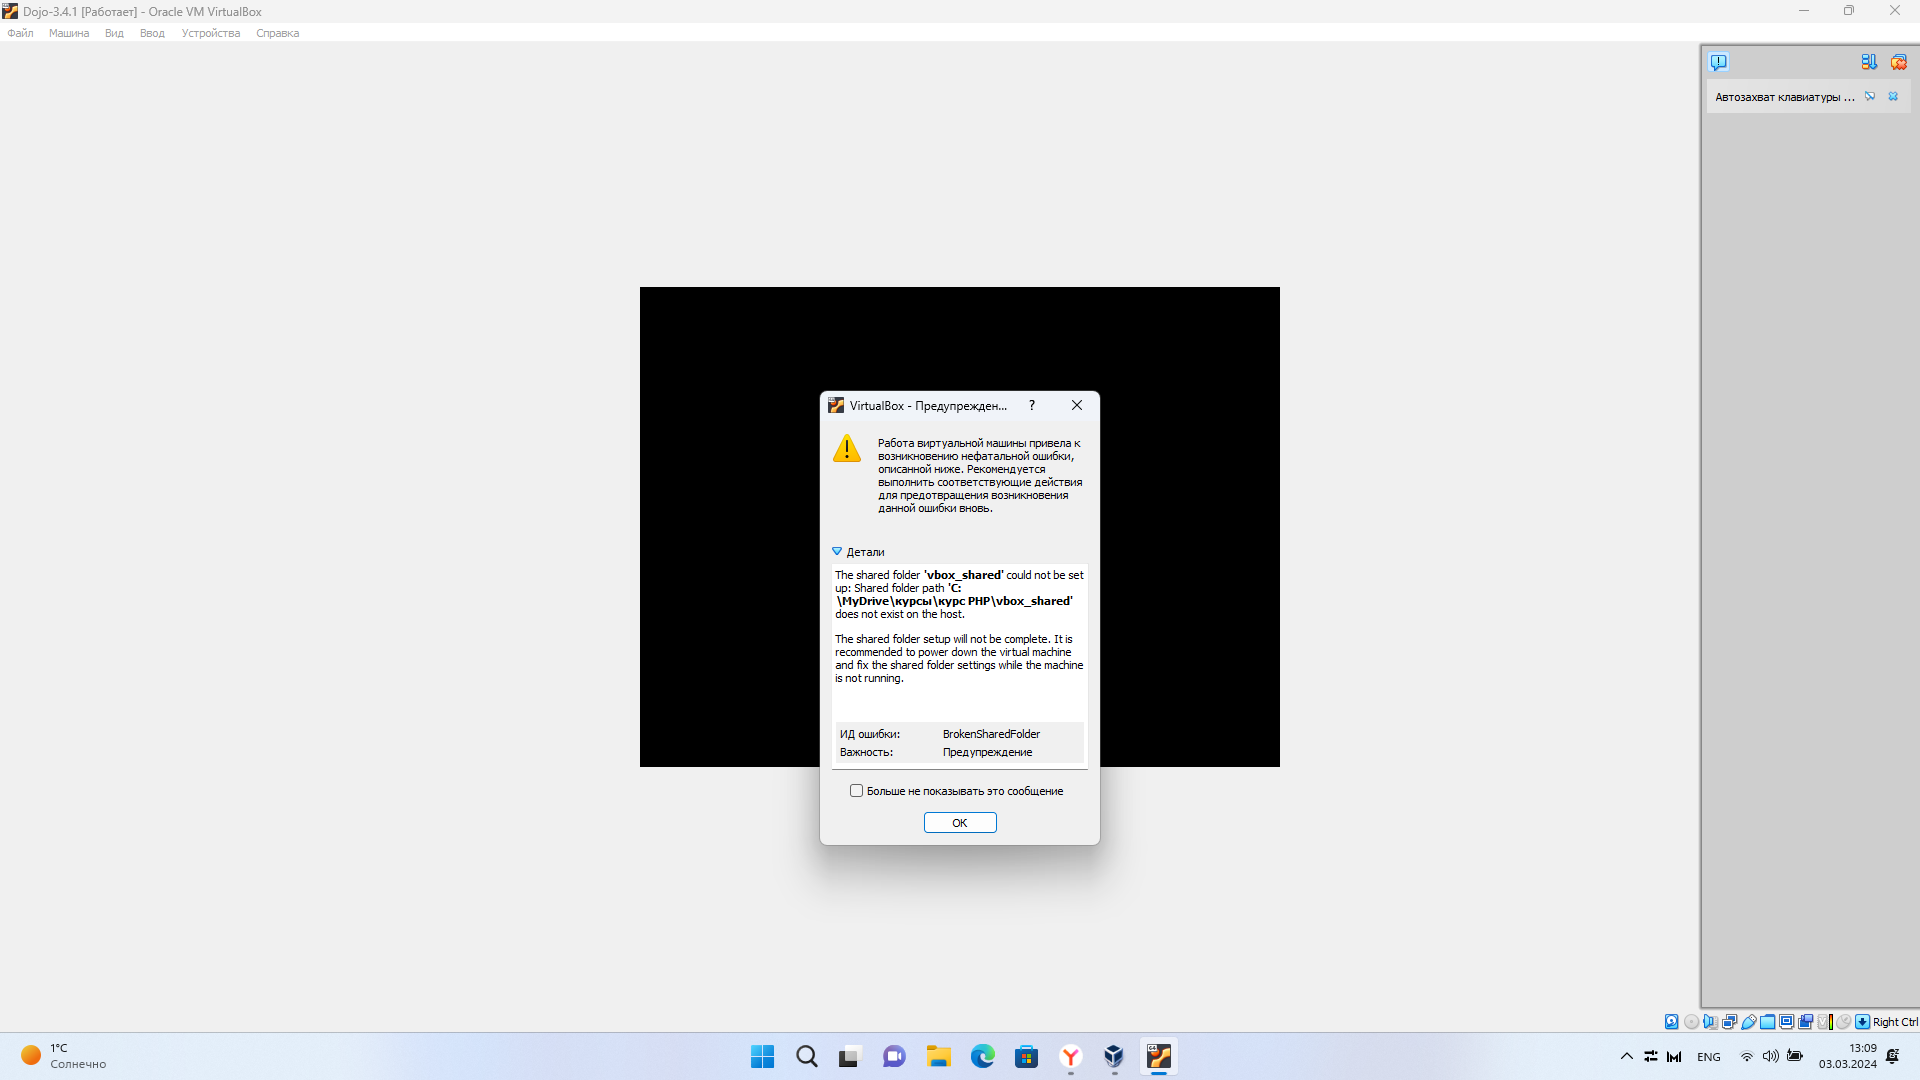
\includegraphics[width=\textwidth]{Screenshot_8}
    \caption{Запускаем виртуальную машину}
  \end{figure}

  \begin{figure}[H]
    \centering
    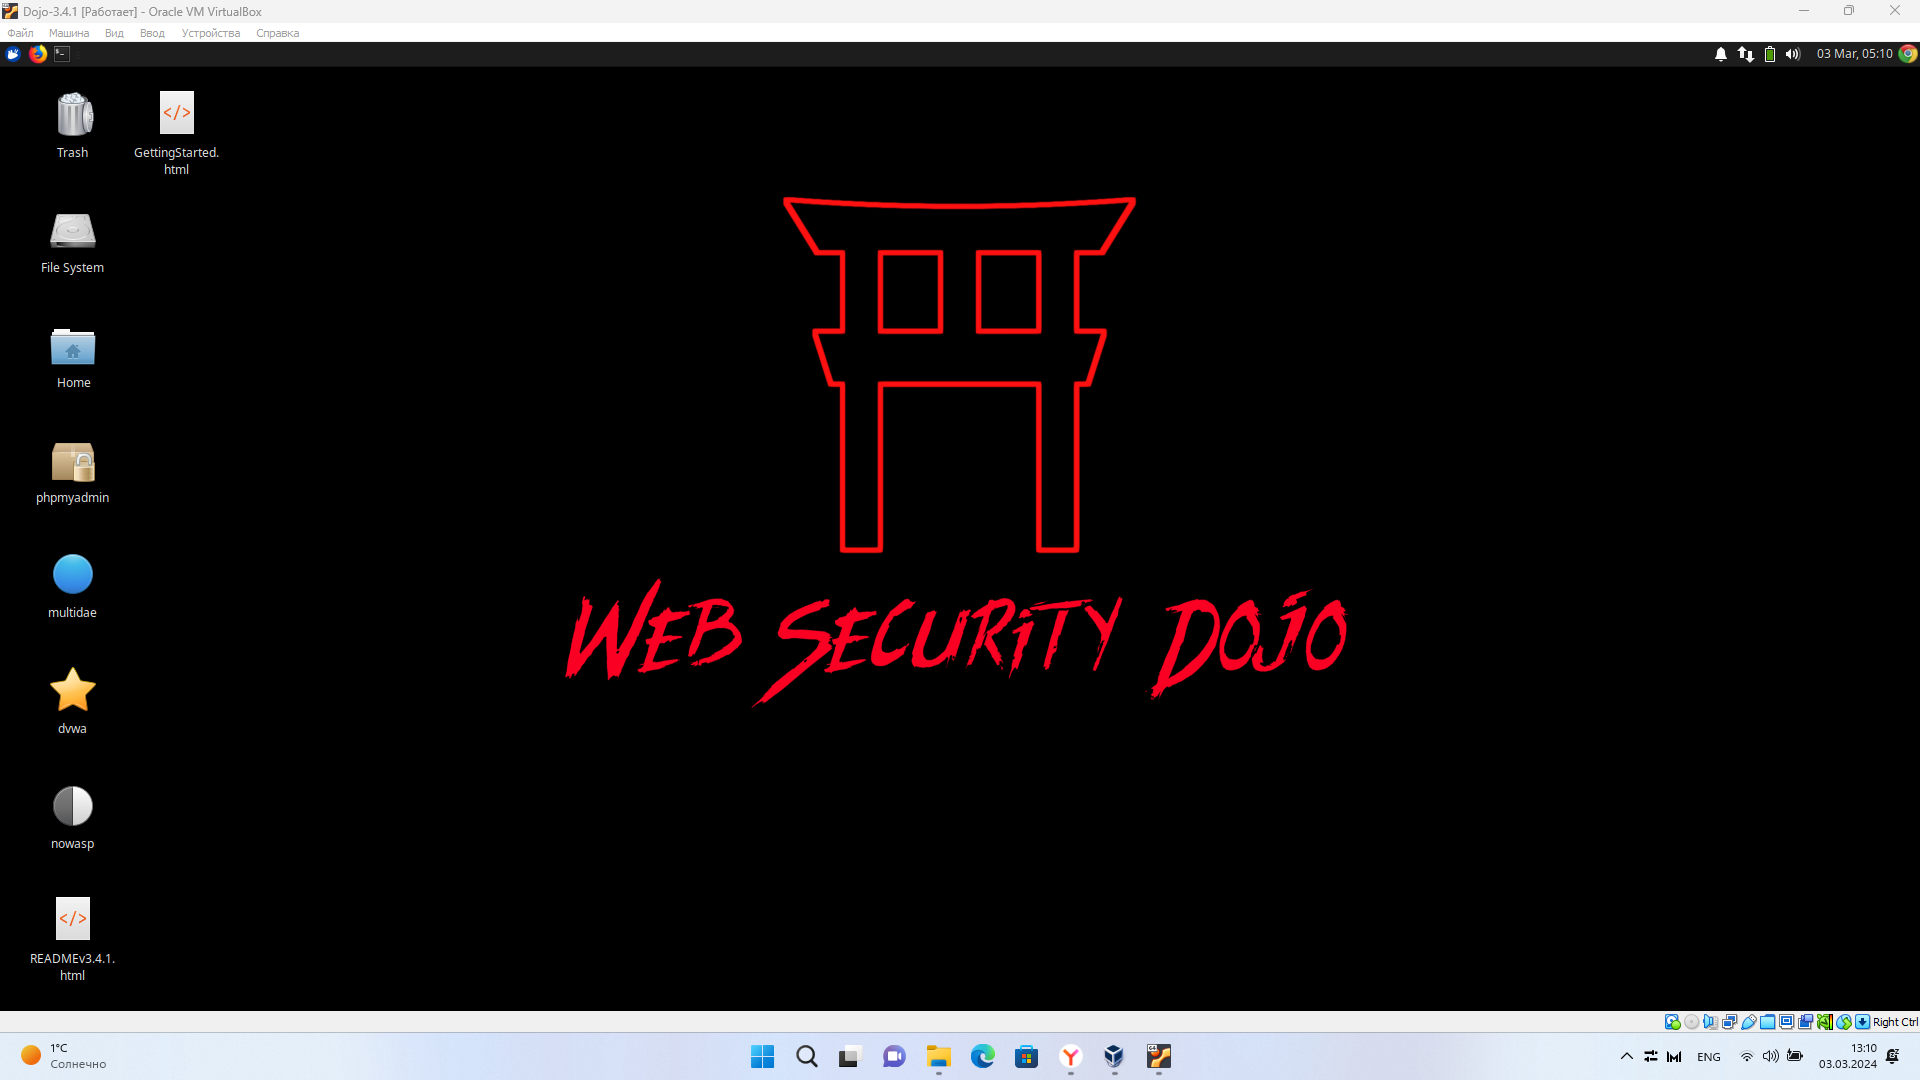
\includegraphics[width=\textwidth]{Screenshot_10}
    \caption{ВМ запущена и готова к работе}
  \end{figure}

  \subsection{Атака на nowasp.local}

  \subsubsection{Авторизация на атакуемом сервисе}

  \begin{figure}[H]
    \centering
    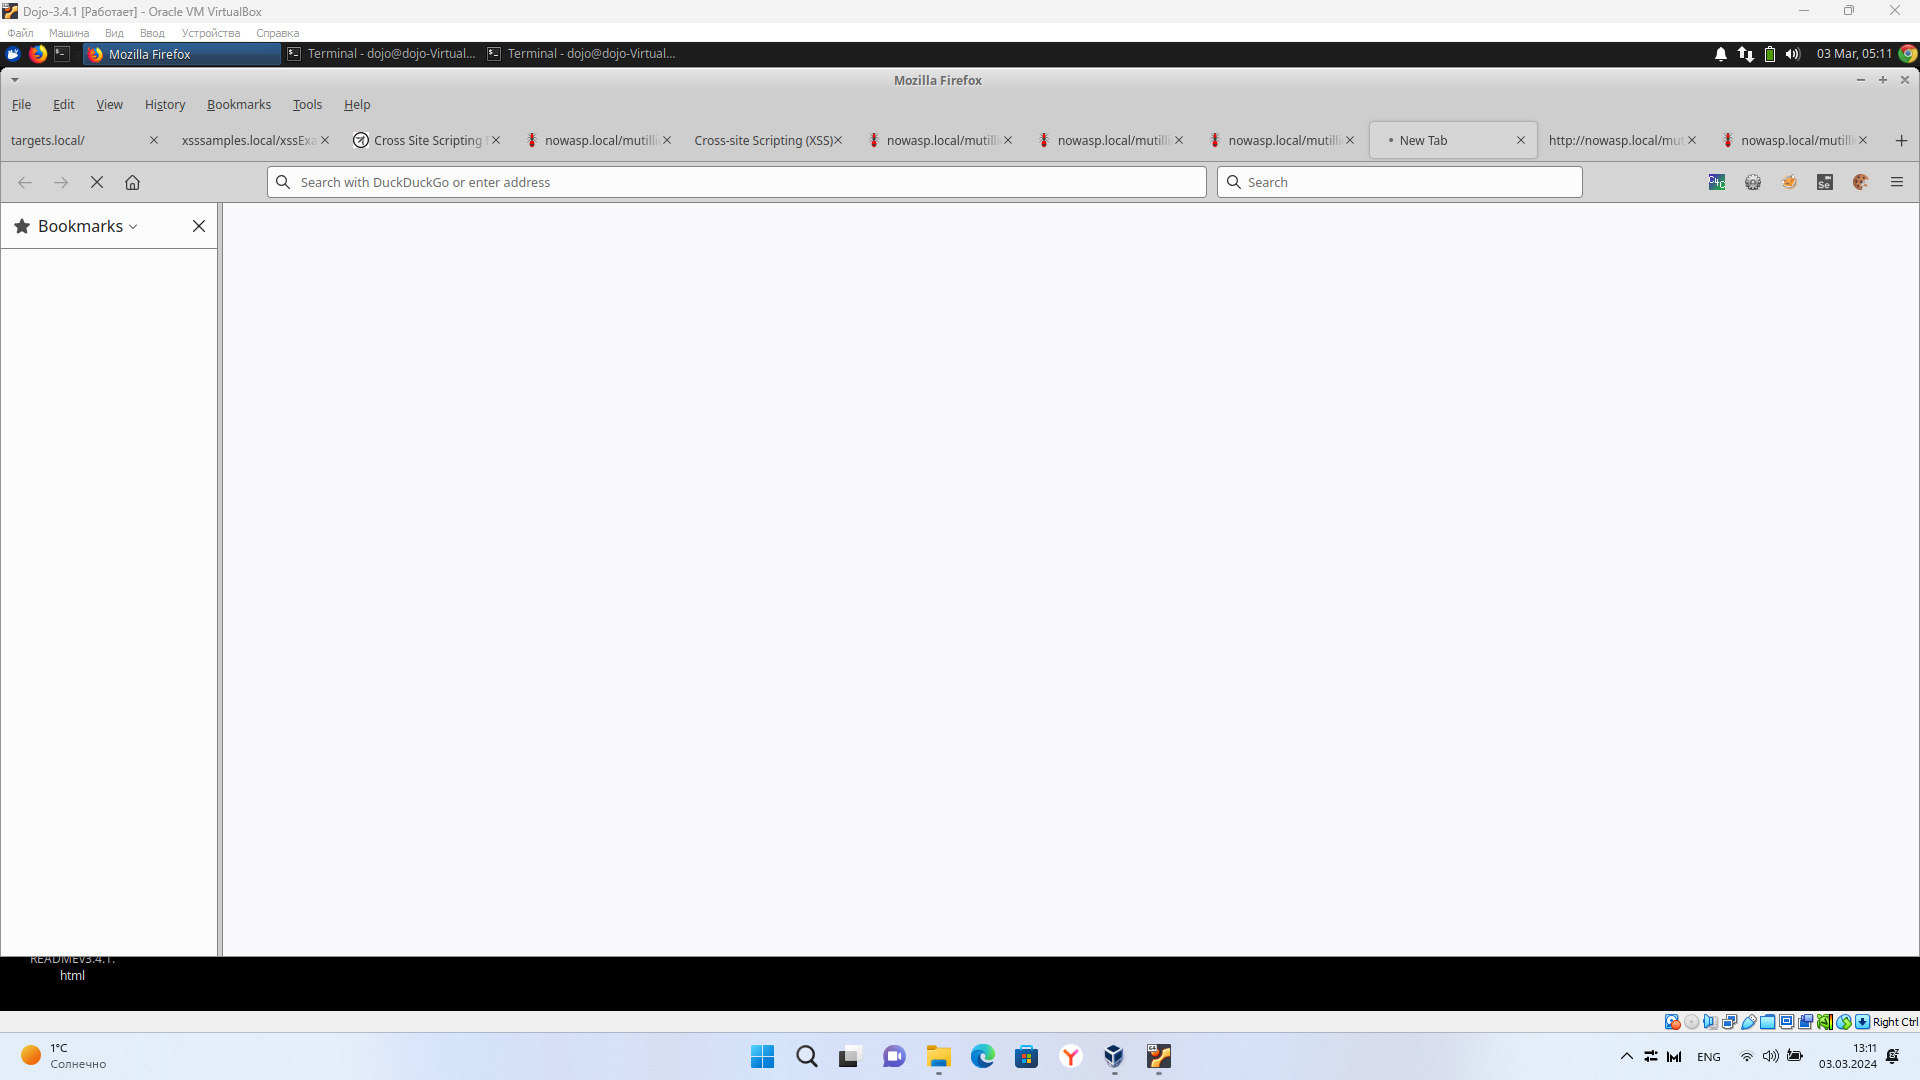
\includegraphics[width=\textwidth]{Screenshot_11}
    \caption{Открываем браузер}
  \end{figure}

  \begin{figure}[H]
    \centering
    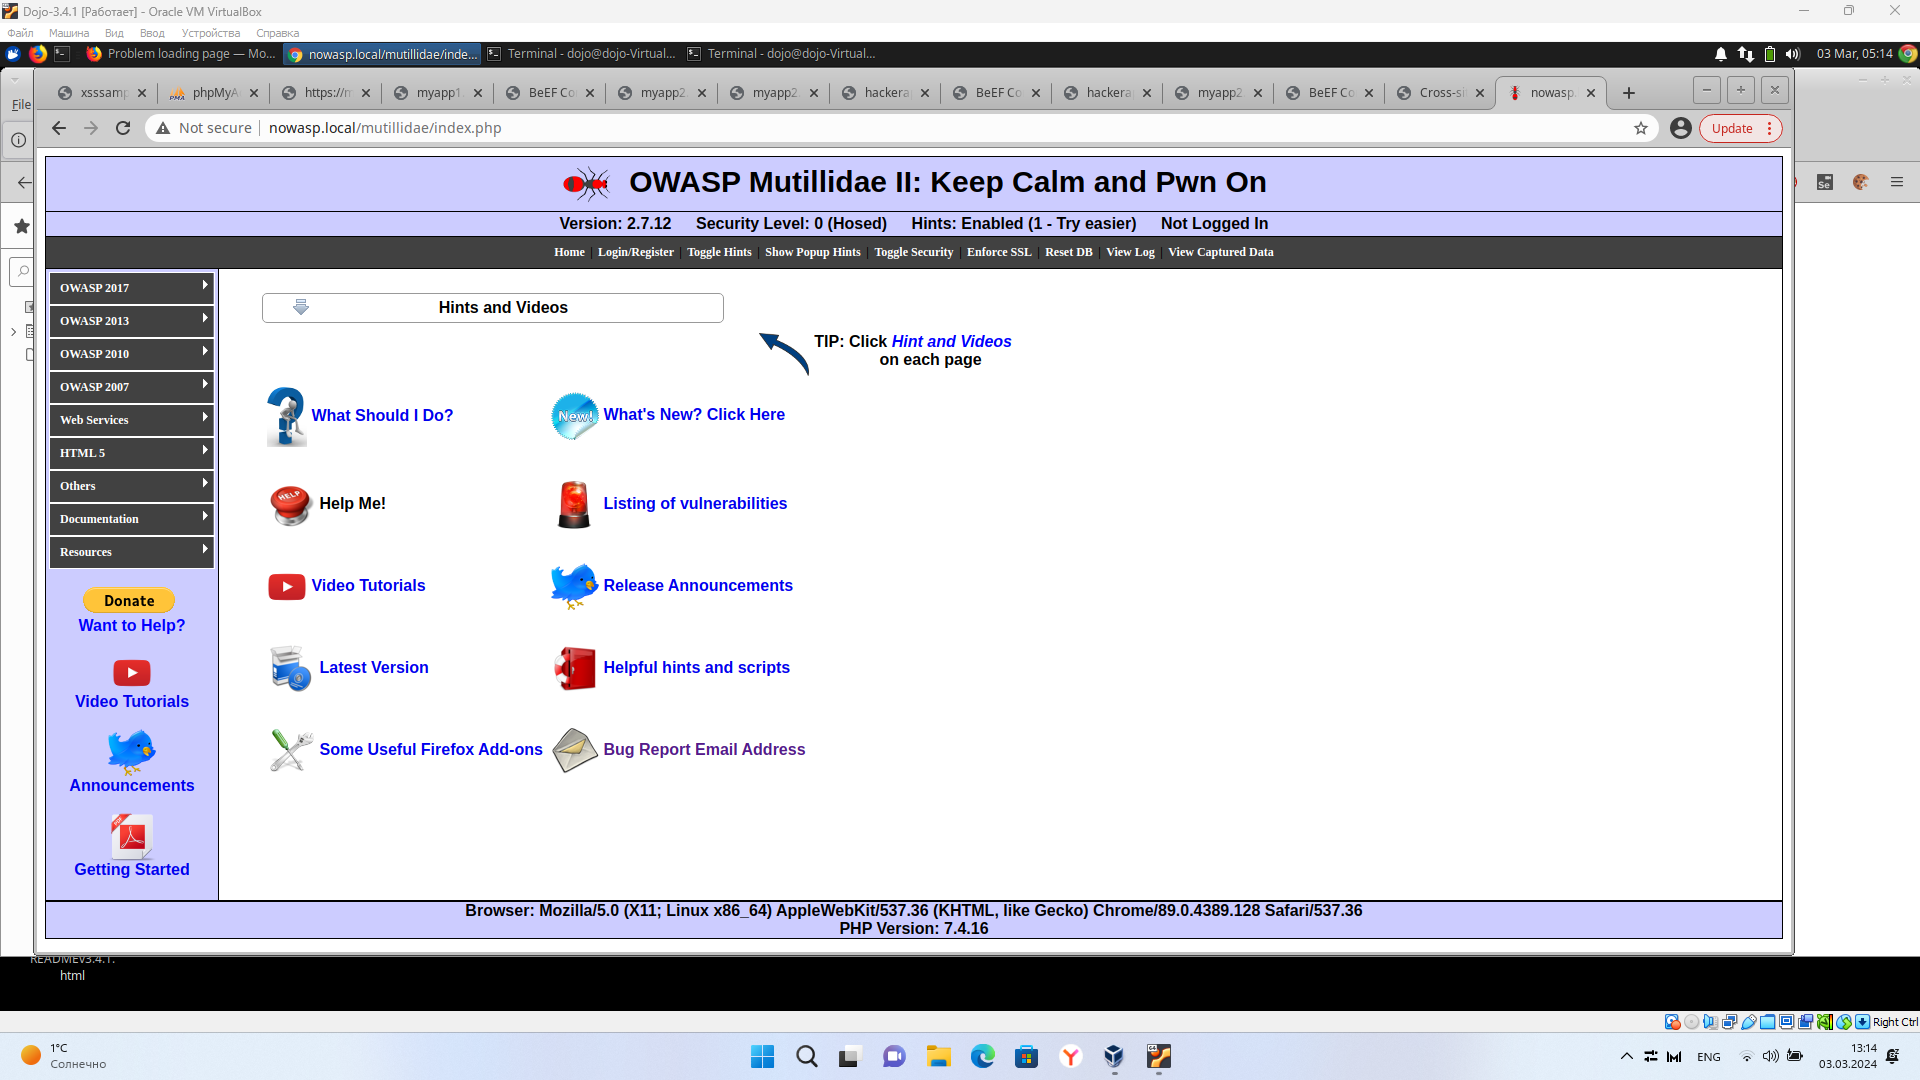
\includegraphics[width=\textwidth]{Screenshot_15}
    \caption{Переходим на сайт для атаки}
  \end{figure}

  \begin{figure}[H]
    \centering
    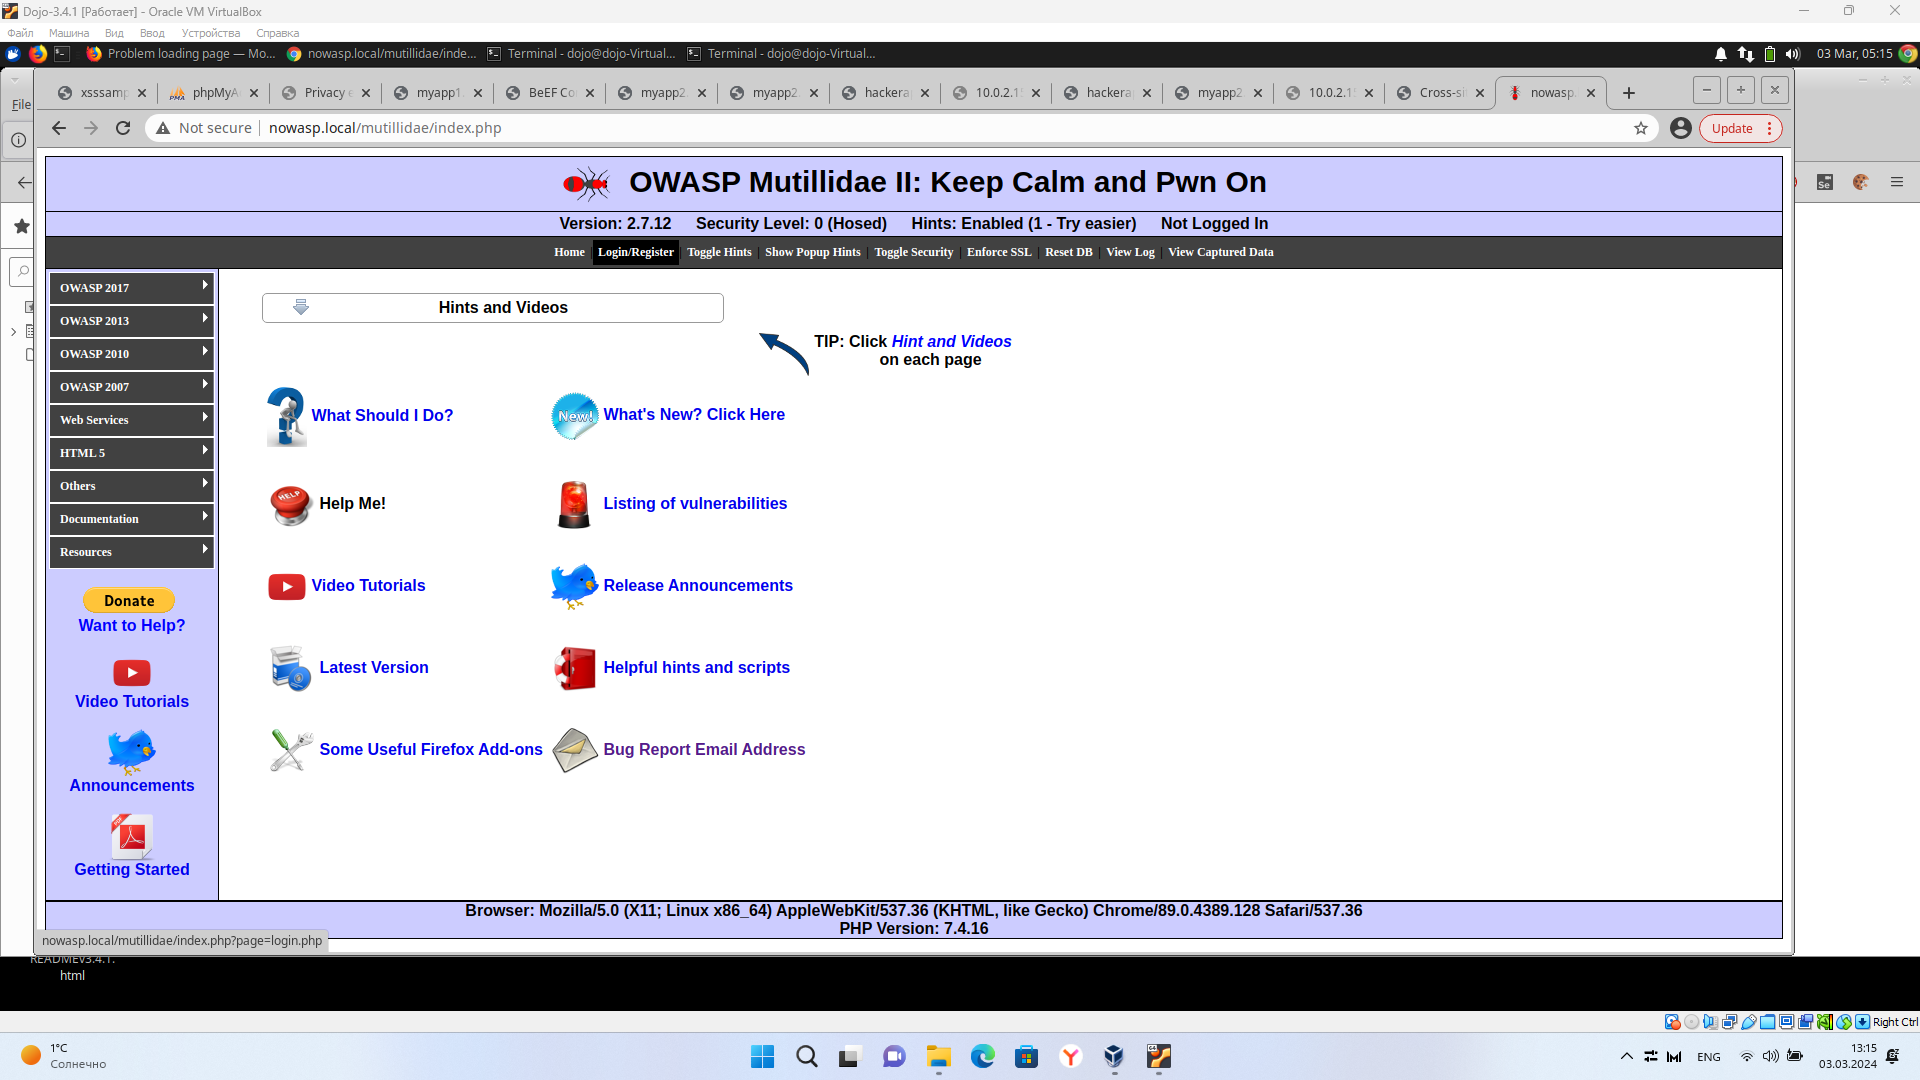
\includegraphics[width=\textwidth]{Screenshot_16}
    \caption{Выполняем вход в учетную запись через кнопку <<Login>>}
  \end{figure}

  \begin{figure}[H]
    \centering
    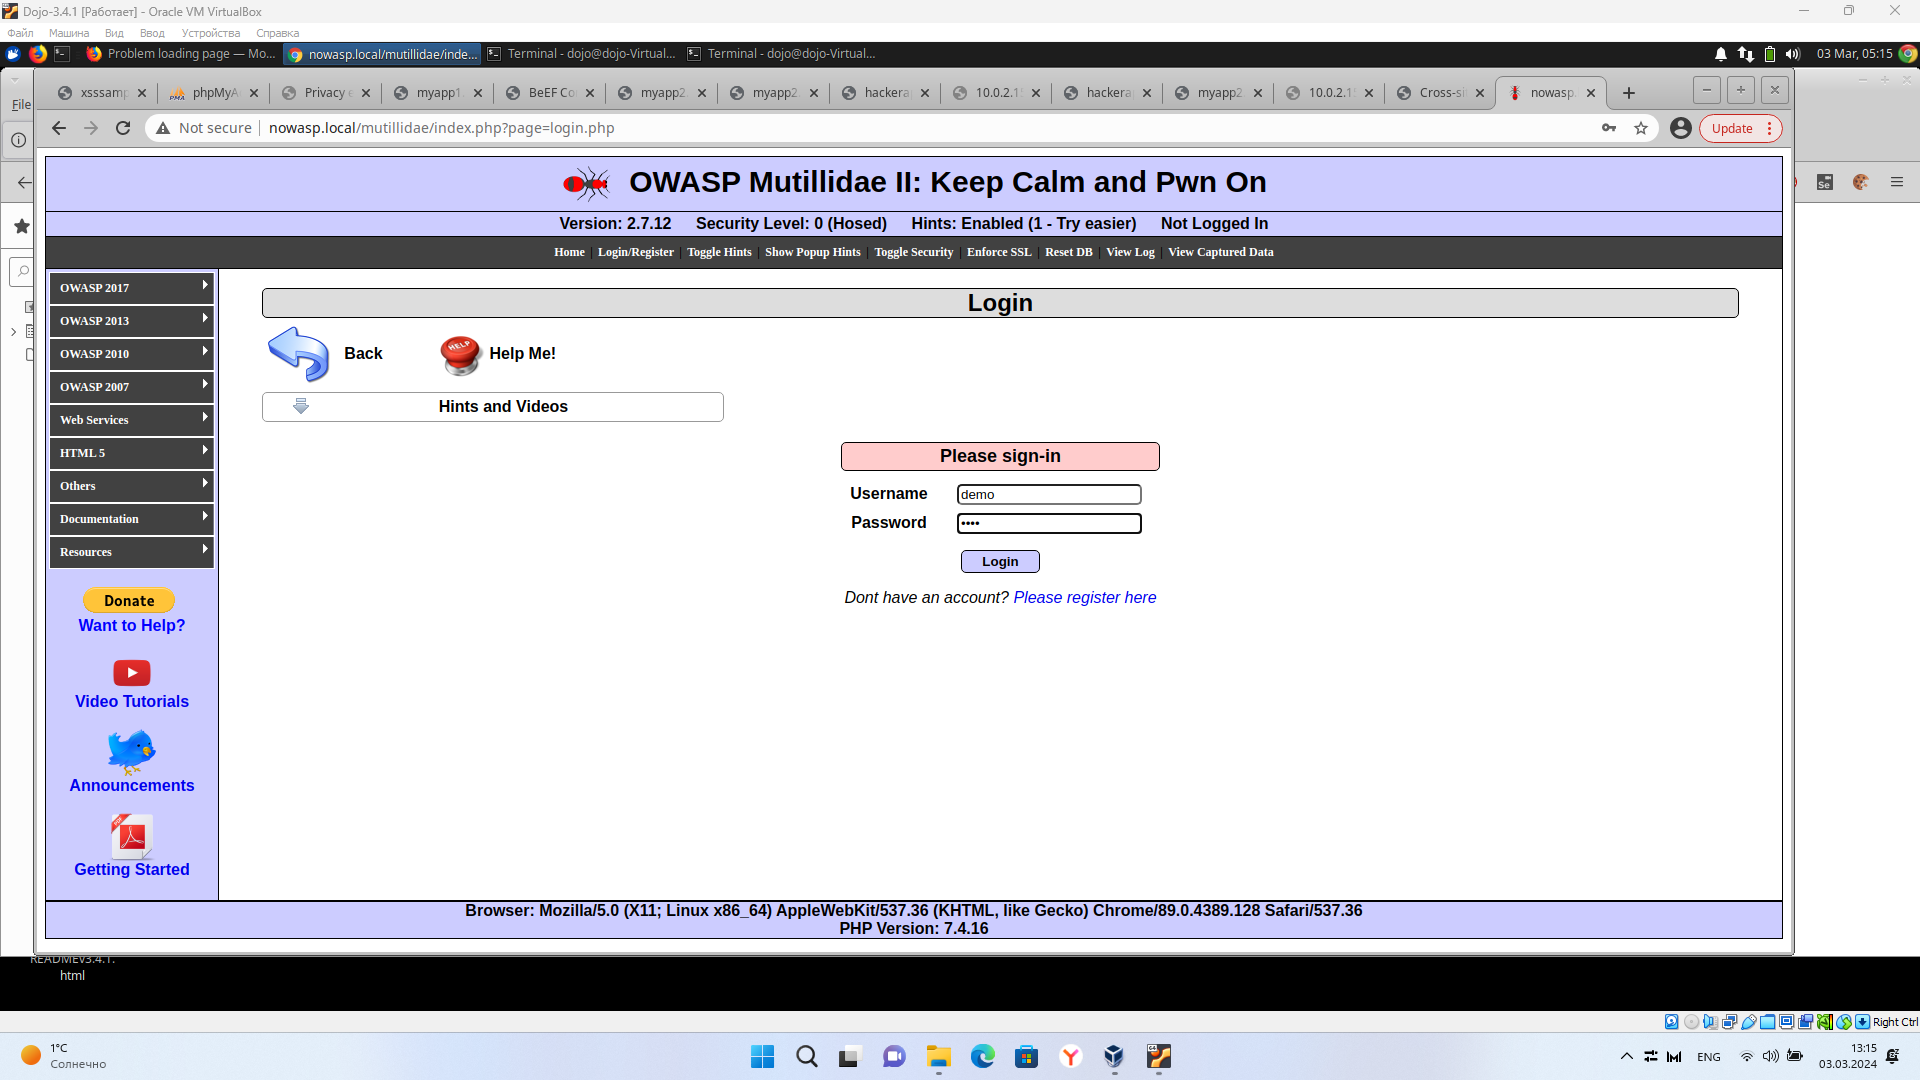
\includegraphics[width=\textwidth]{Screenshot_17}
    \caption{Вводим логин и пароль}
  \end{figure}

  \begin{figure}[H]
    \centering
    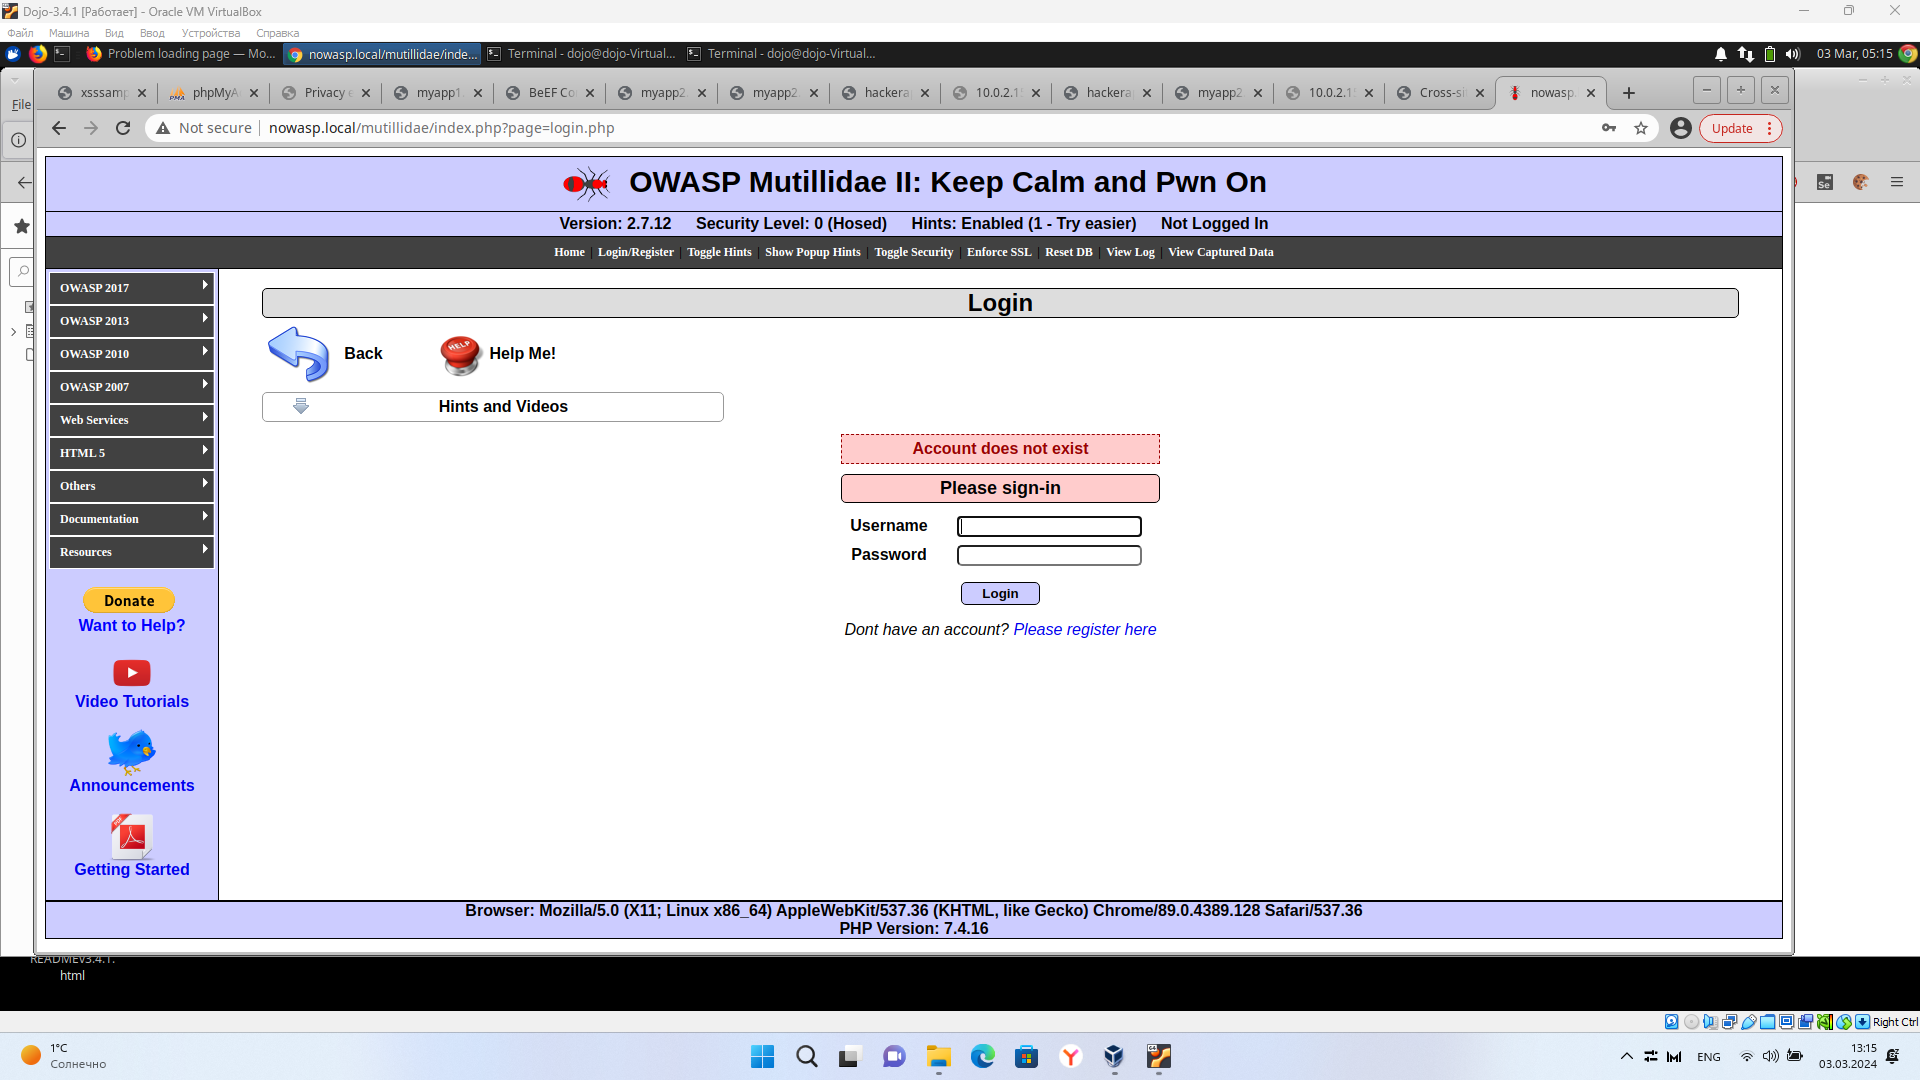
\includegraphics[width=\textwidth]{Screenshot_18}
    \caption{Стандартные учетные данные не подходят}
  \end{figure}

  \begin{figure}[H]
    \centering
    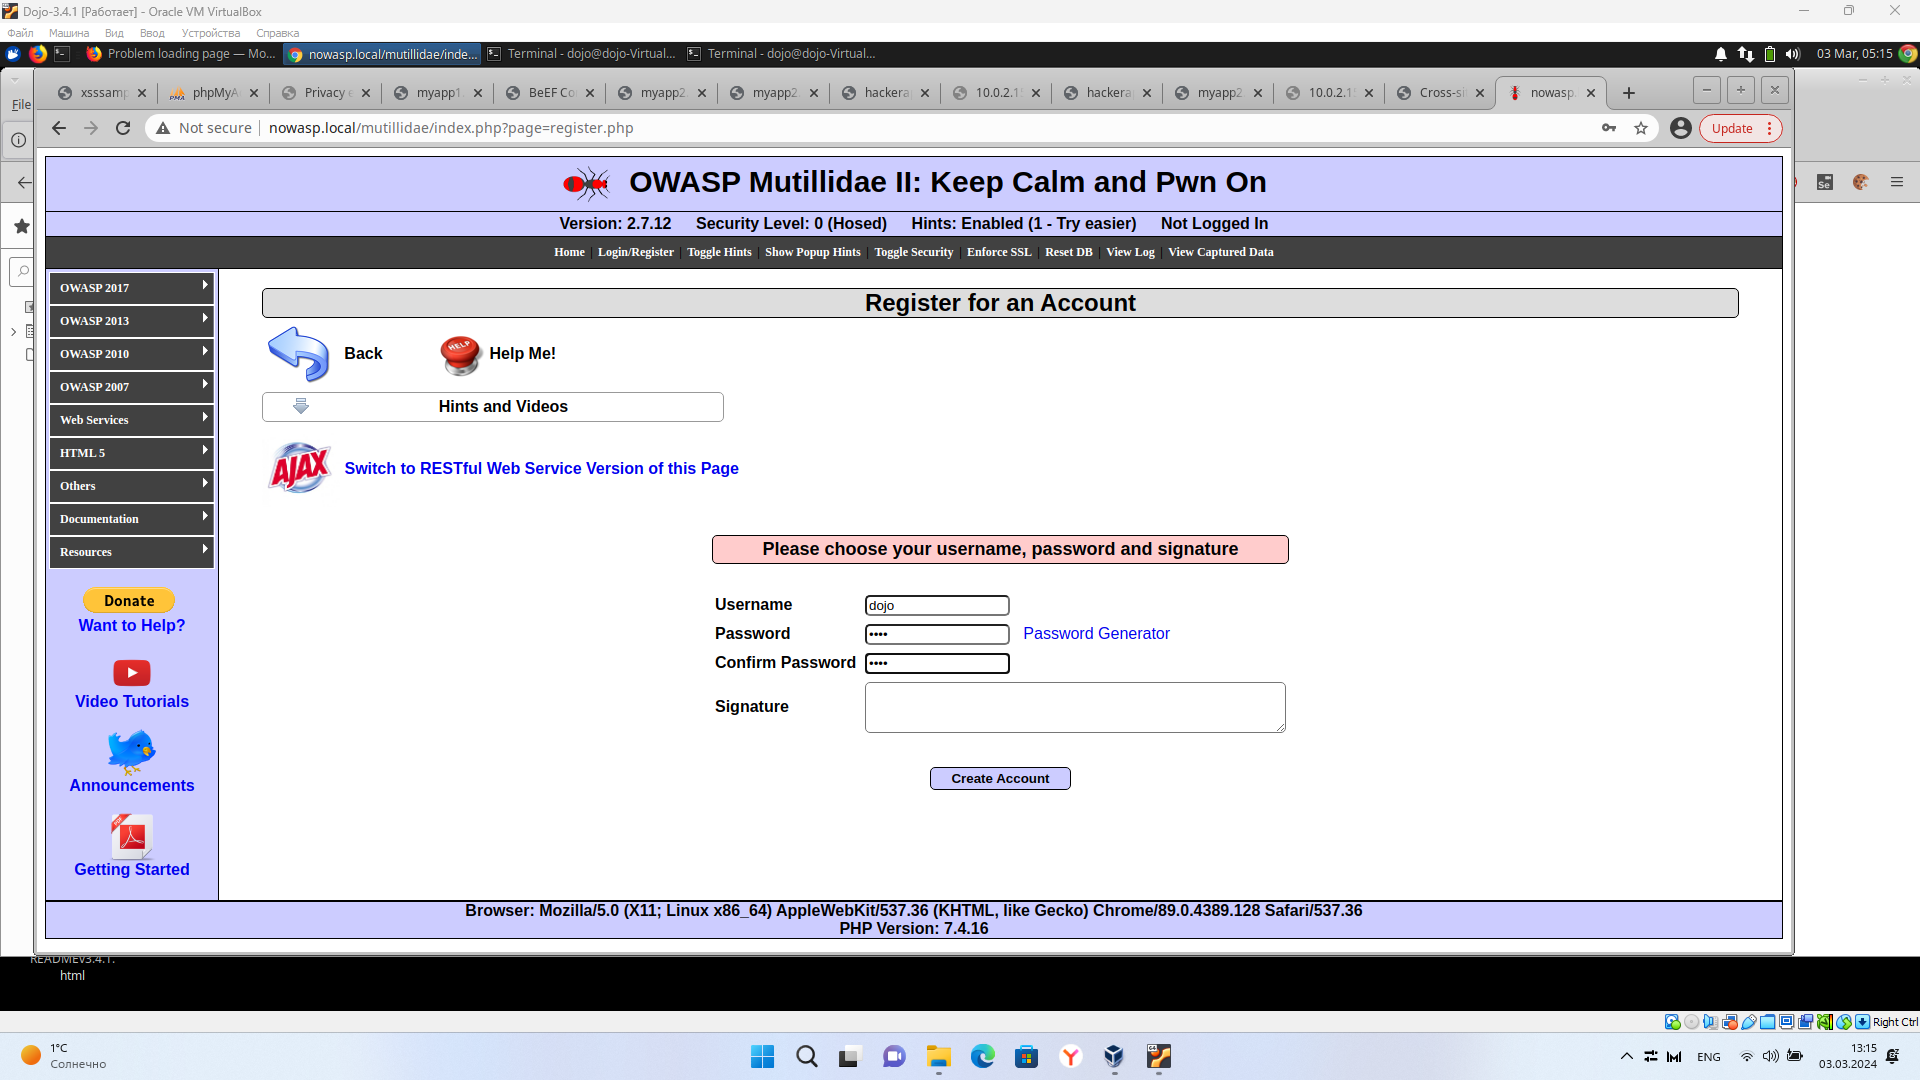
\includegraphics[width=\textwidth]{Screenshot_19}
    \caption{Необходимо зарегестрировать нового пользователя}
  \end{figure}

  \begin{figure}[H]
    \centering
    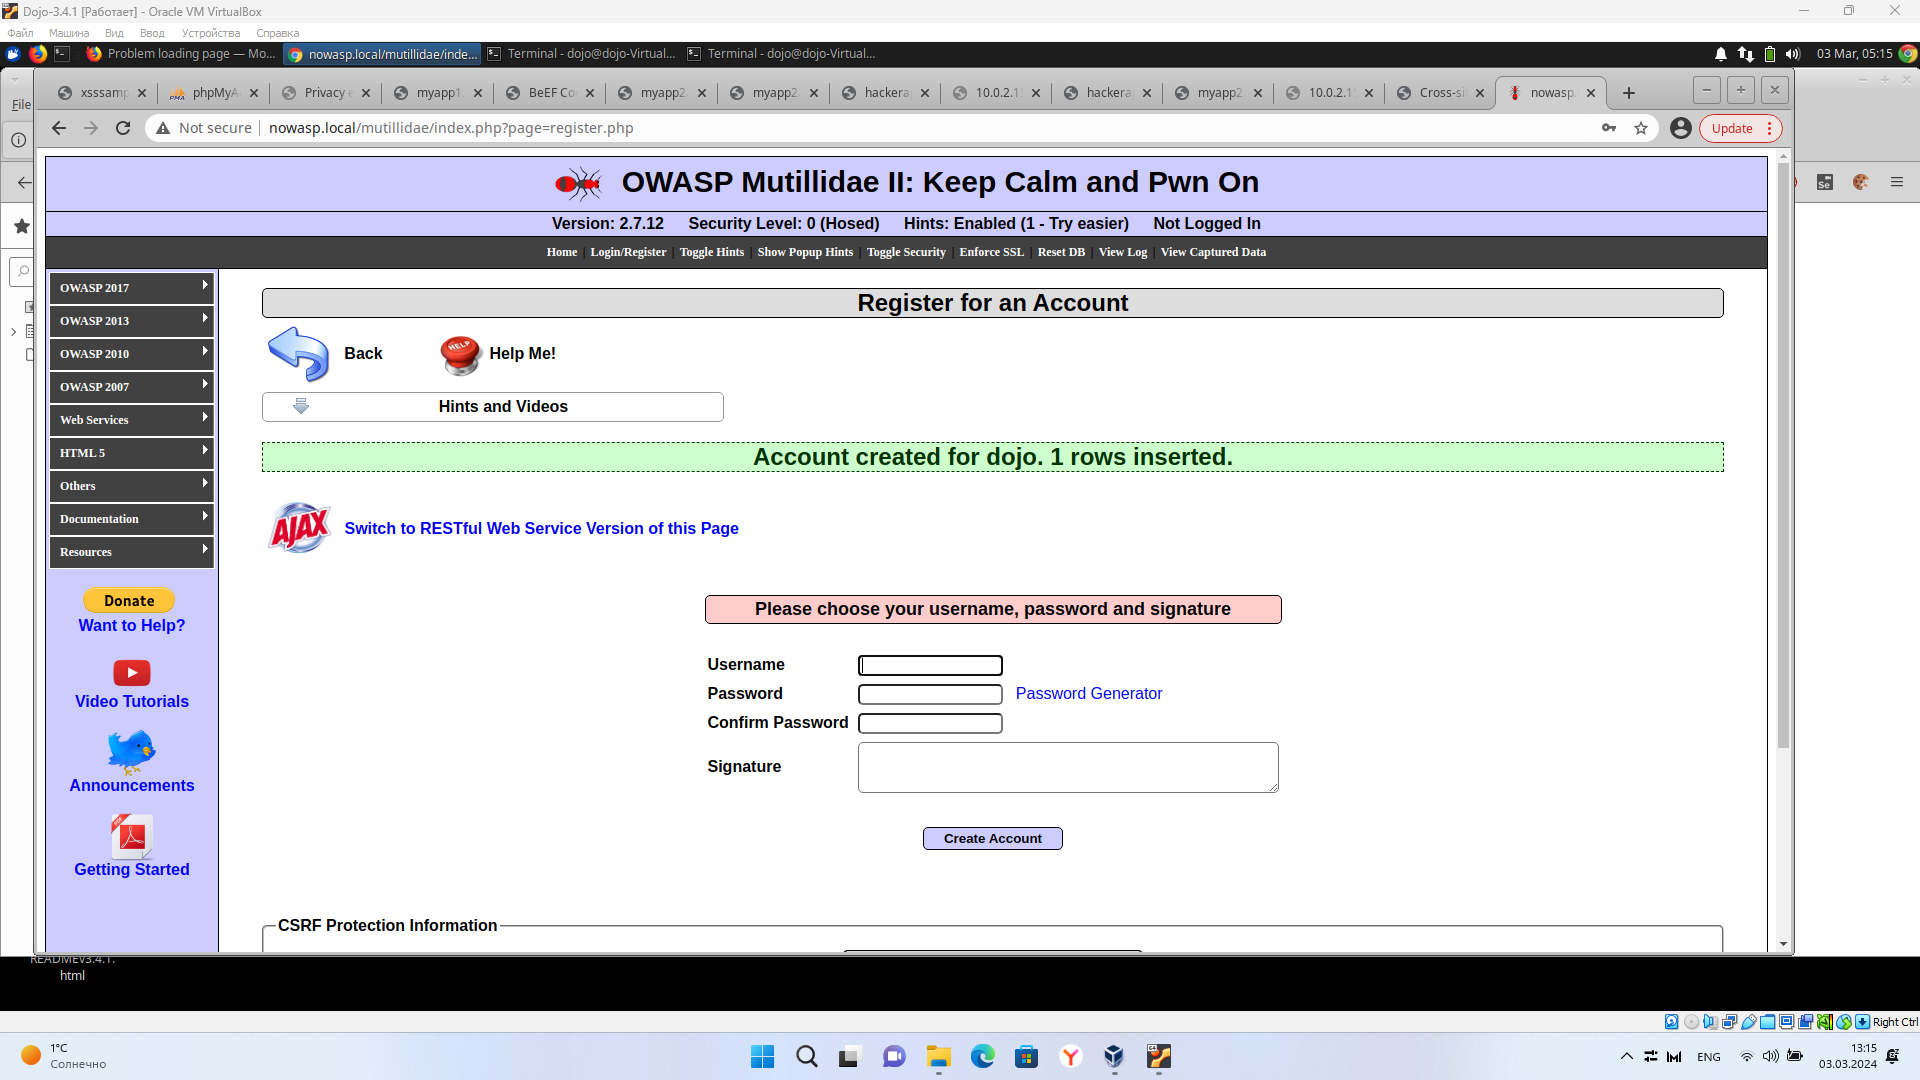
\includegraphics[width=\textwidth]{Screenshot_20}
    \caption{Новый пользователь создан}
  \end{figure}

  \begin{figure}[H]
    \centering
    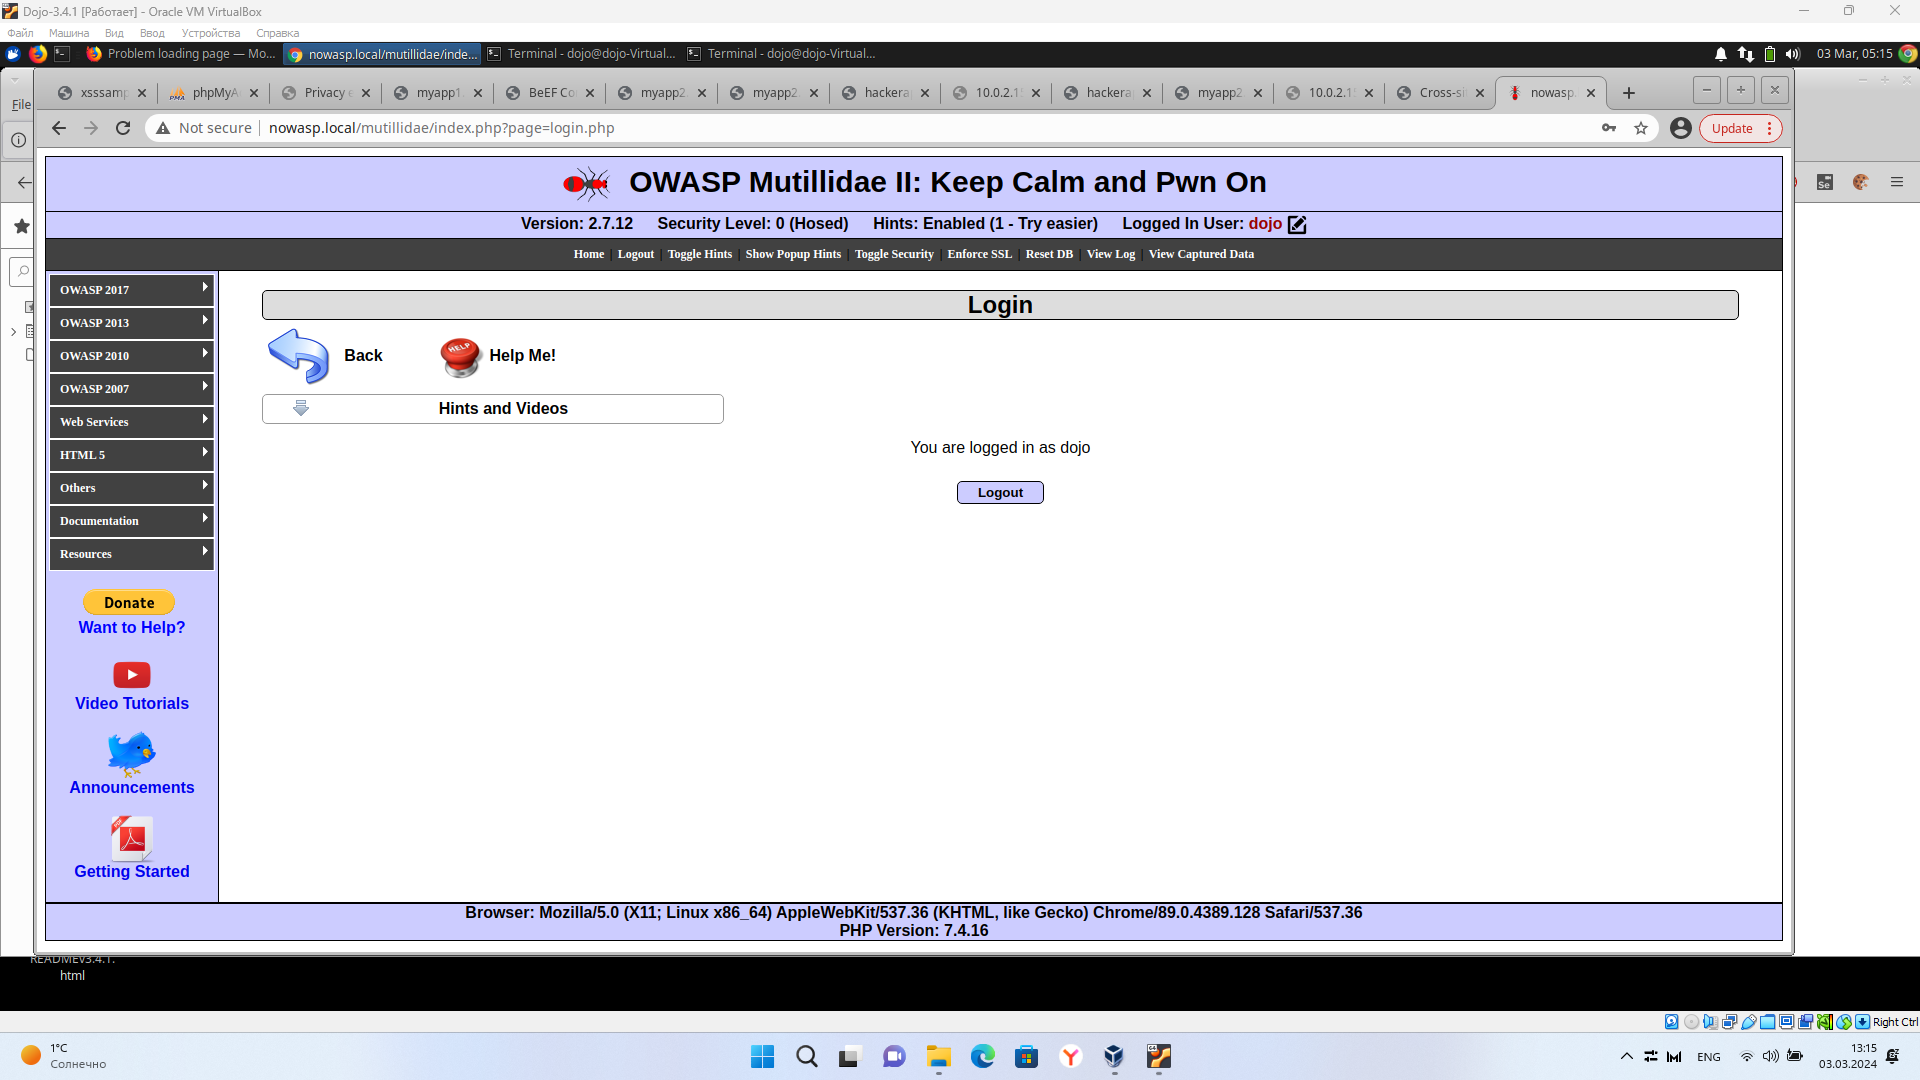
\includegraphics[width=\textwidth]{Screenshot_21}
    \caption{Переходим на страницу входы}
  \end{figure}

  \begin{figure}[H]
    \centering
    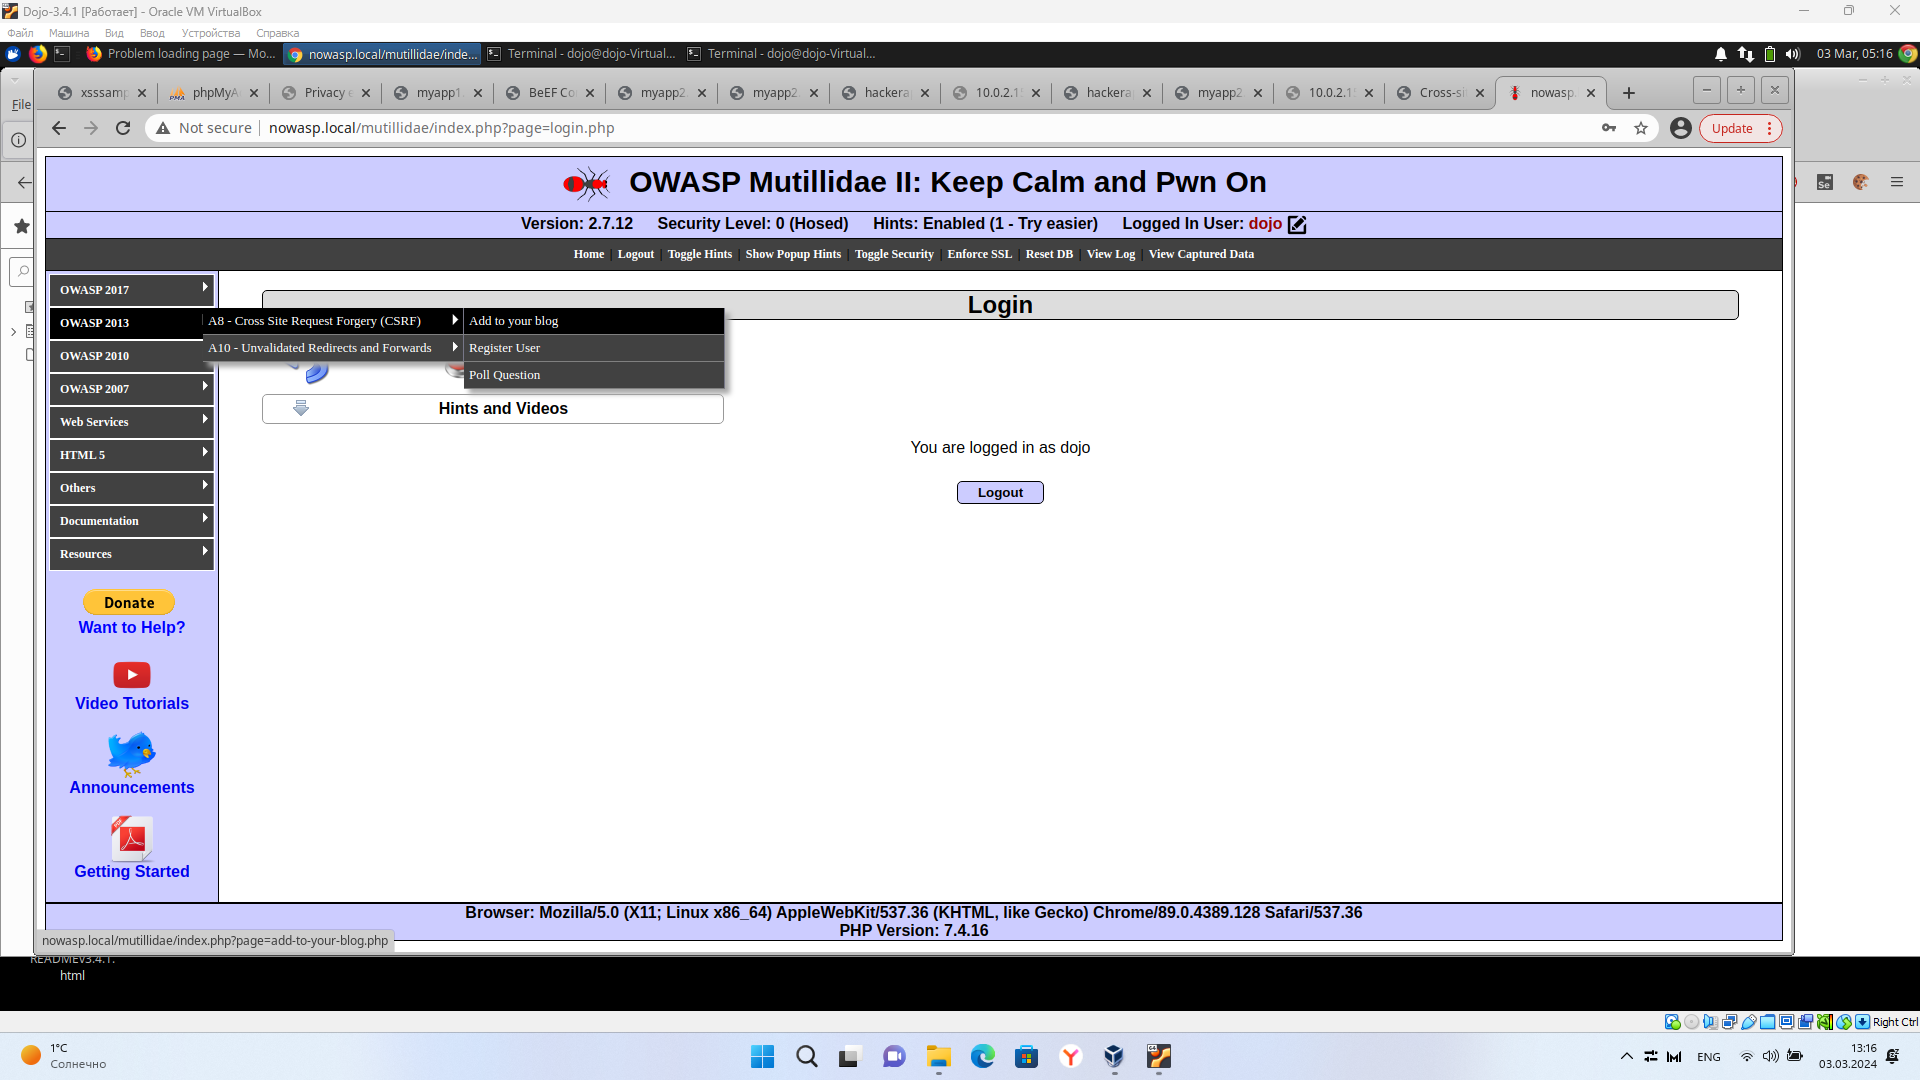
\includegraphics[width=\textwidth]{Screenshot_22}
    \caption{Вход на сайт выполнен успешно}
  \end{figure}

  \subsubsection{Анализ атакуемой странице}

  \begin{figure}[H]
    \centering
    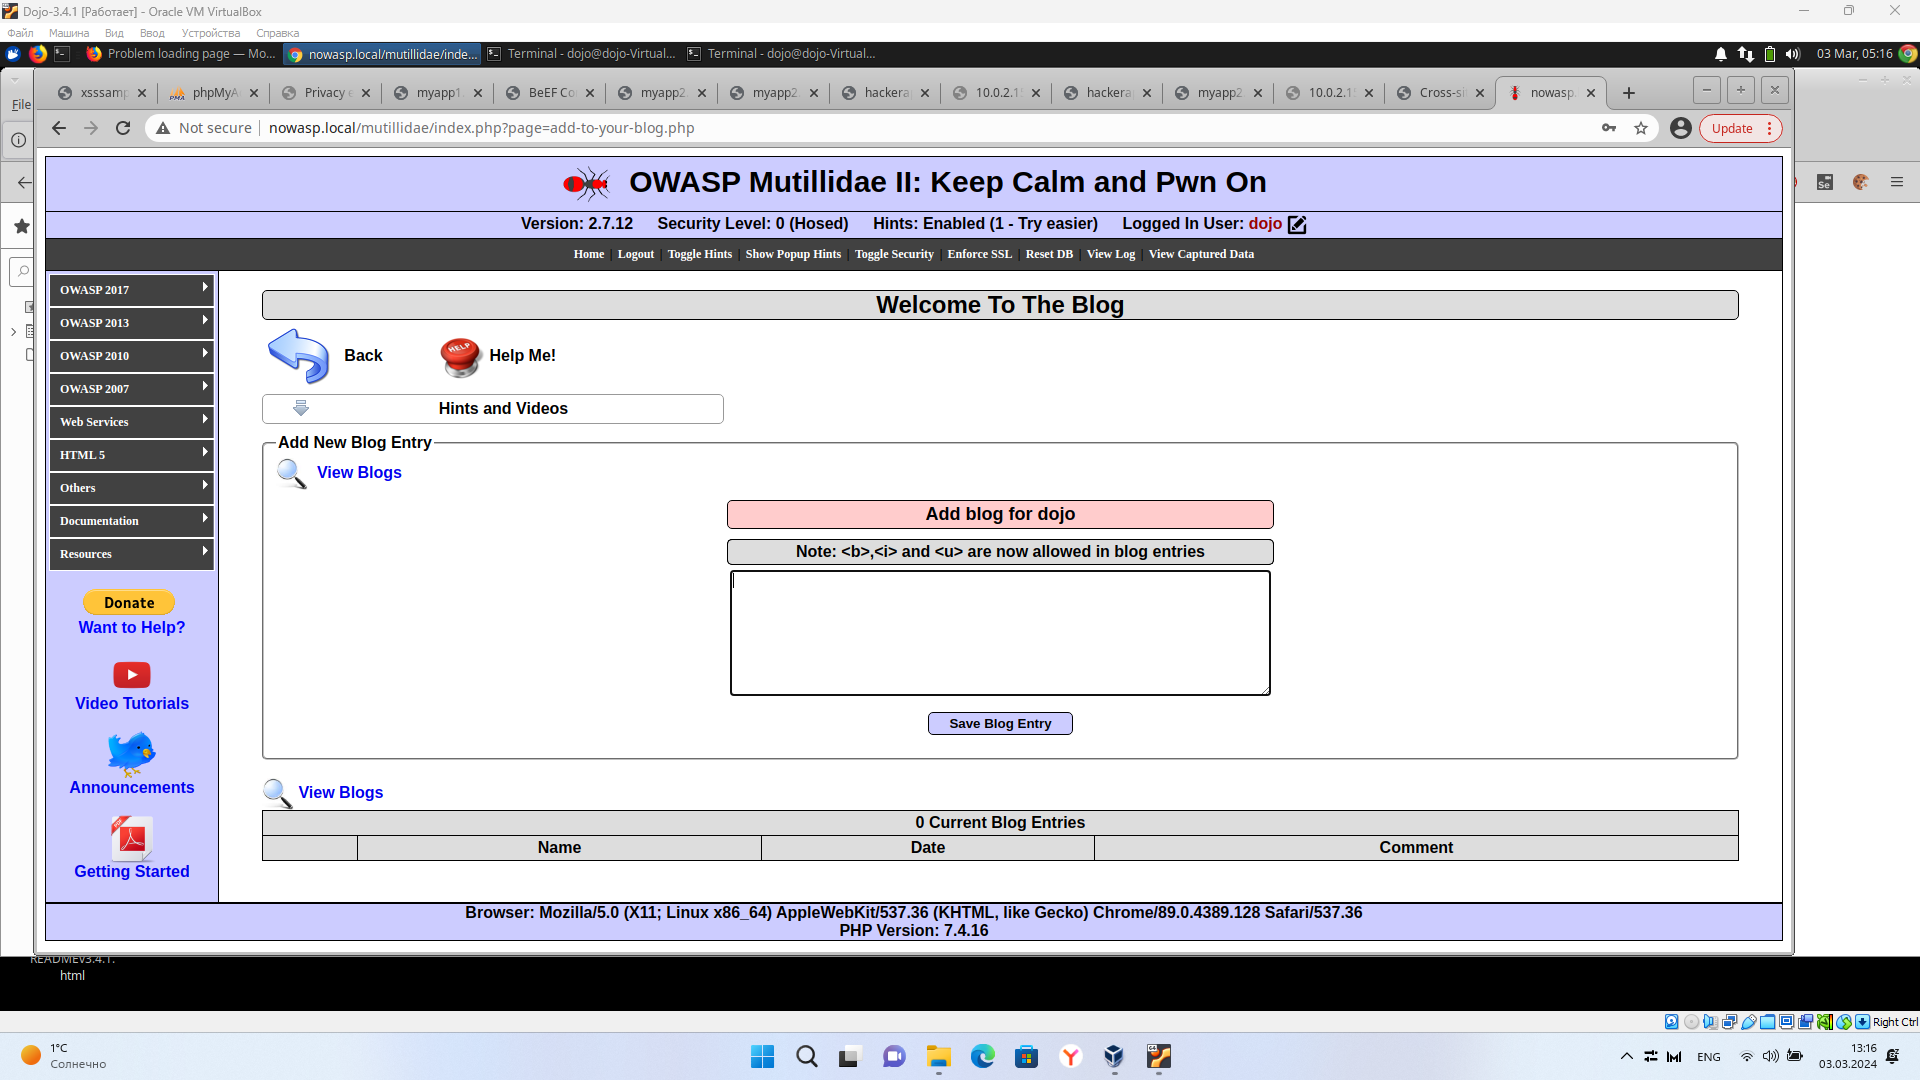
\includegraphics[width=\textwidth]{Screenshot_23}
    \caption{Открываем атакуемую страницу - добавление нового поста}
  \end{figure}

  \begin{figure}[H]
    \centering
    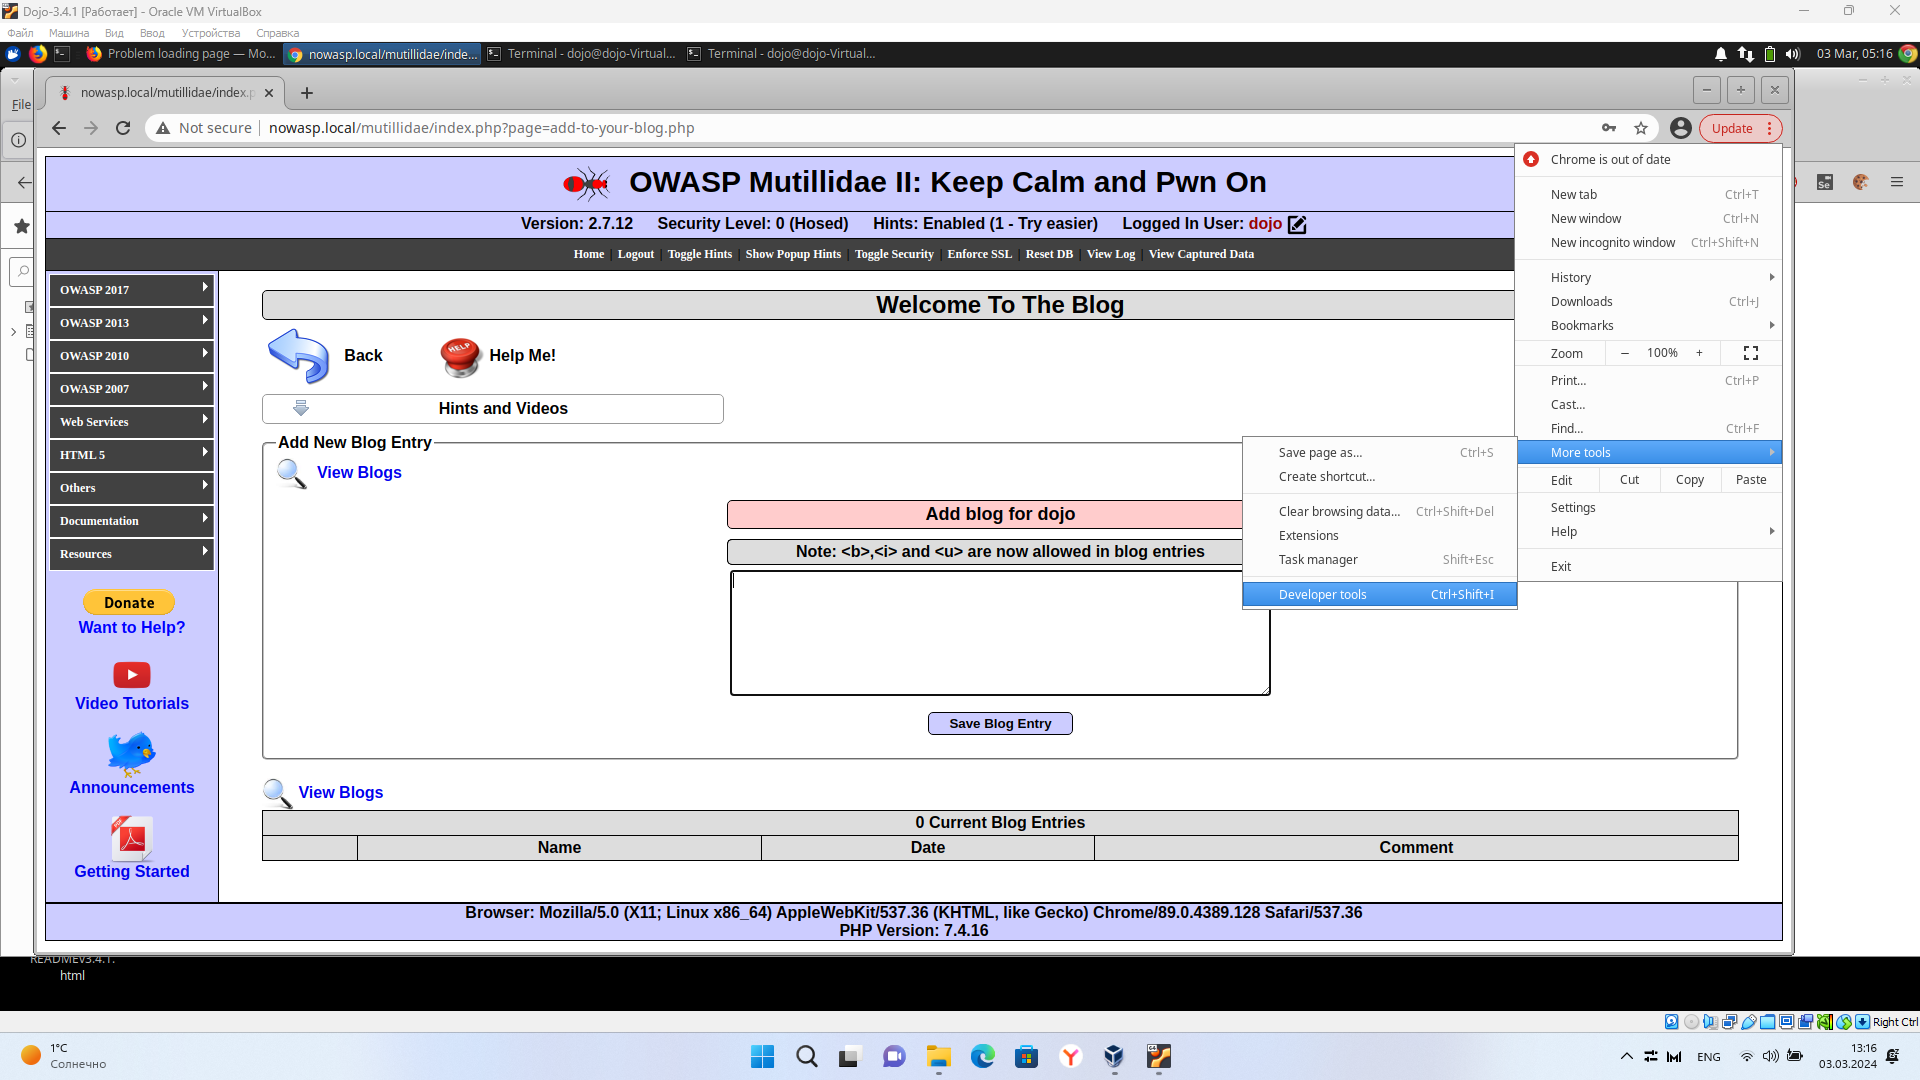
\includegraphics[width=\textwidth]{Screenshot_24}
    \caption{Открываем инструменты разработчика для анализа}
  \end{figure}

  \begin{figure}[H]
    \centering
    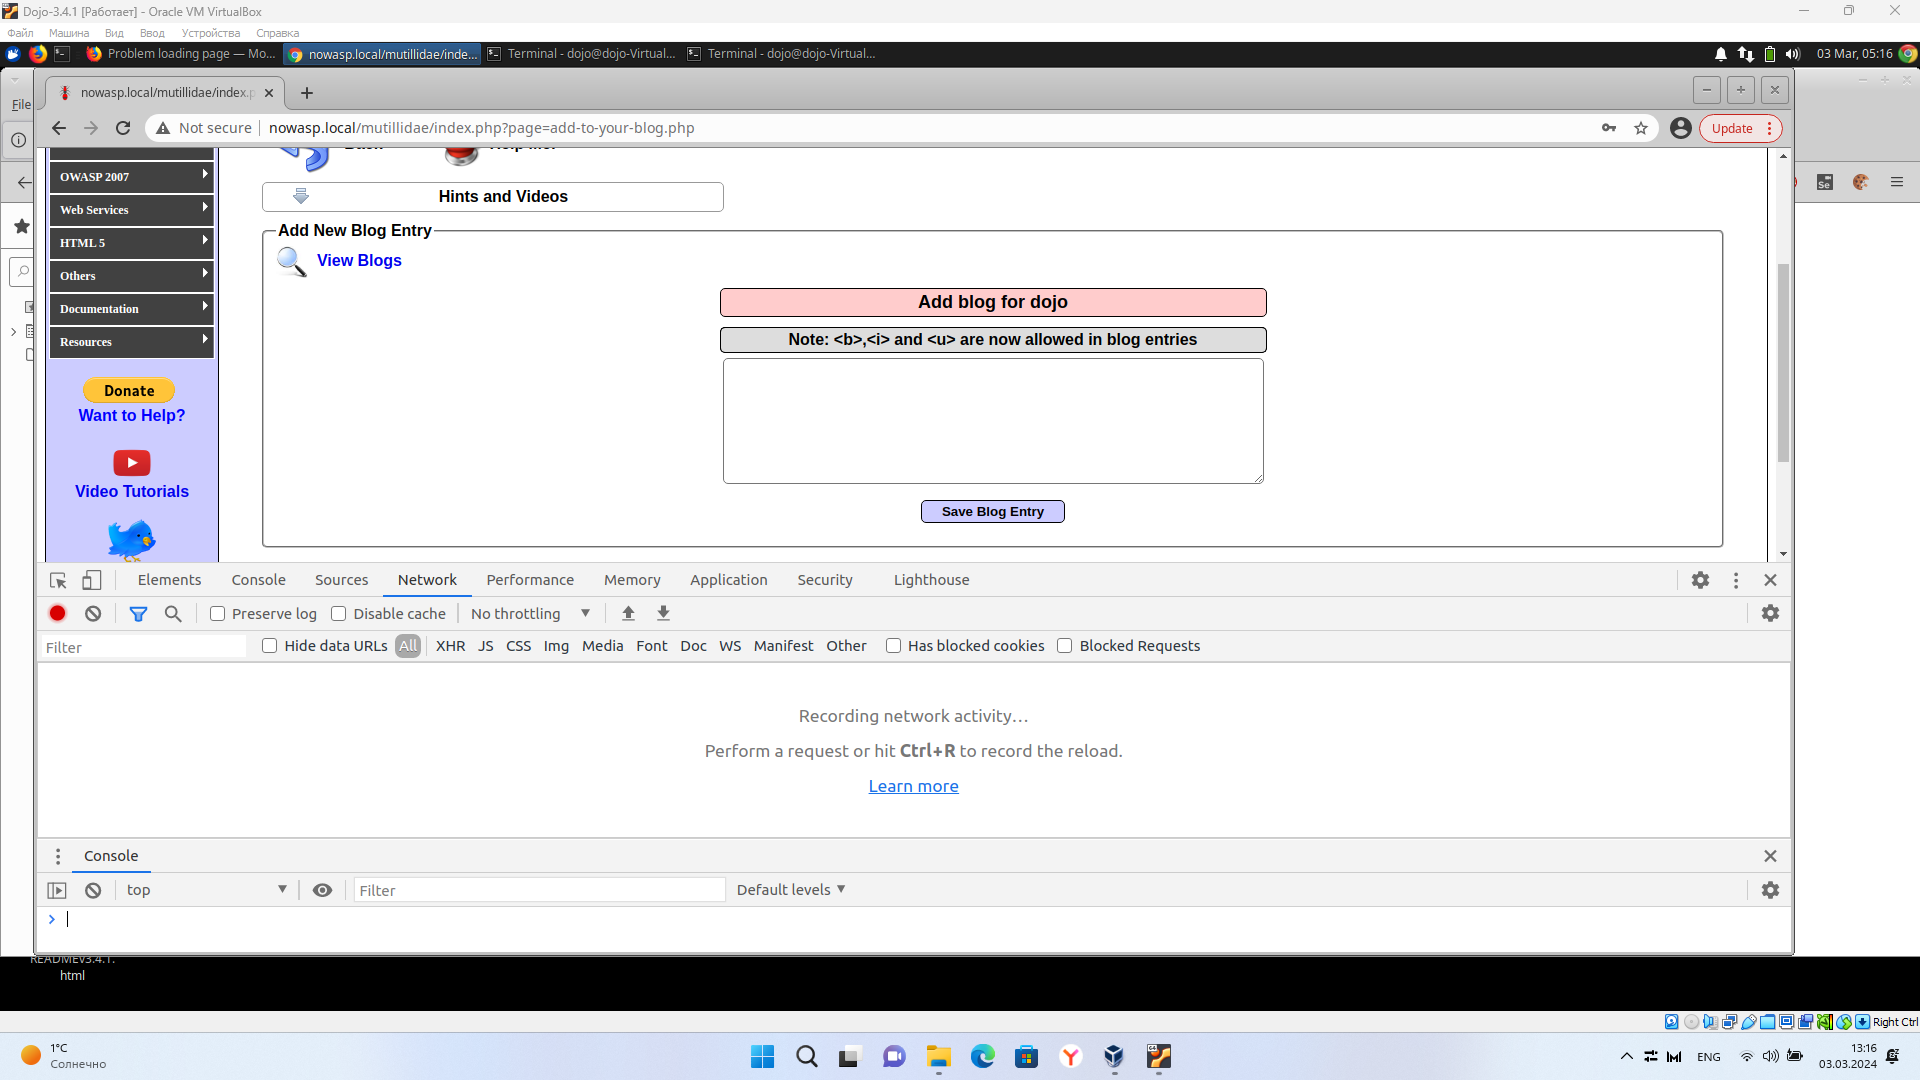
\includegraphics[width=\textwidth]{Screenshot_25}
    \caption{Открываем вкладку анализа сетевых запросов}
  \end{figure}

  \begin{figure}[H]
    \centering
    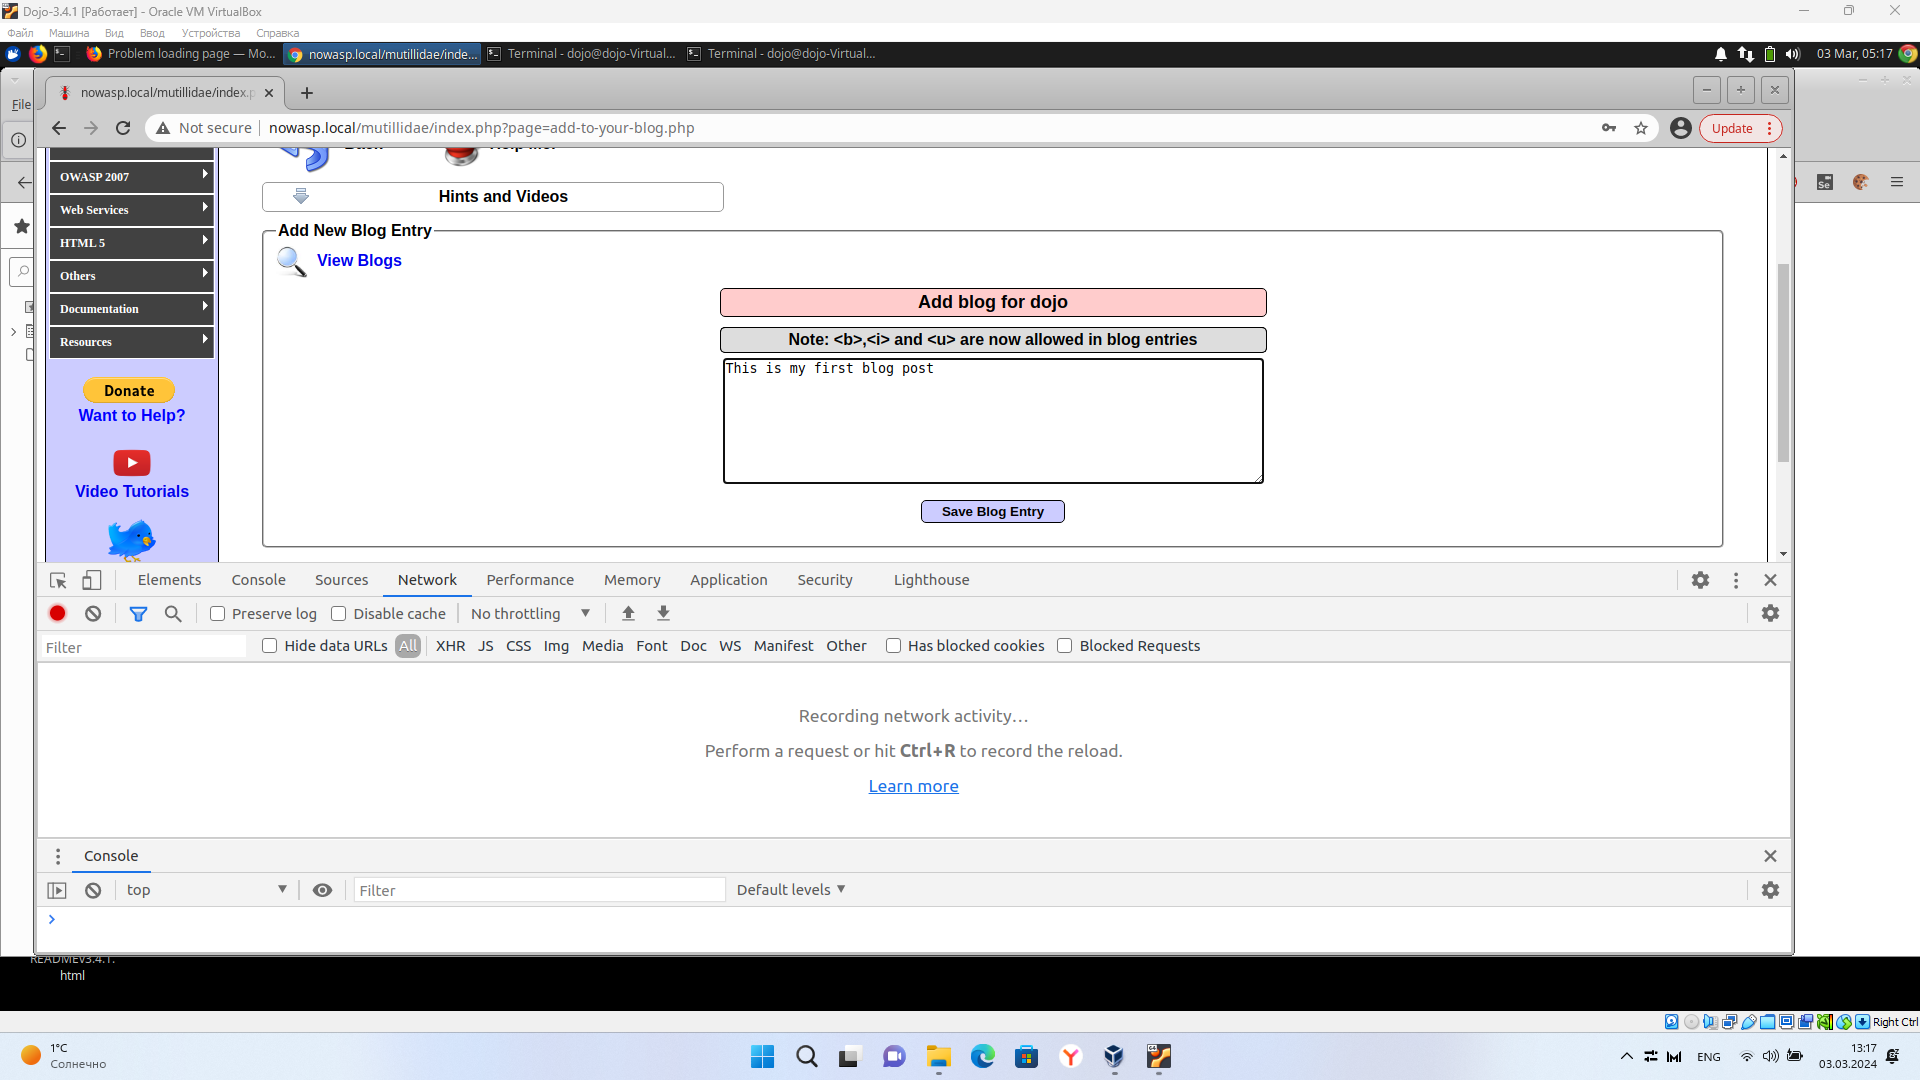
\includegraphics[width=\textwidth]{Screenshot_26}
    \caption{Вводим текст для нового поста}
  \end{figure}

  \begin{figure}[H]
    \centering
    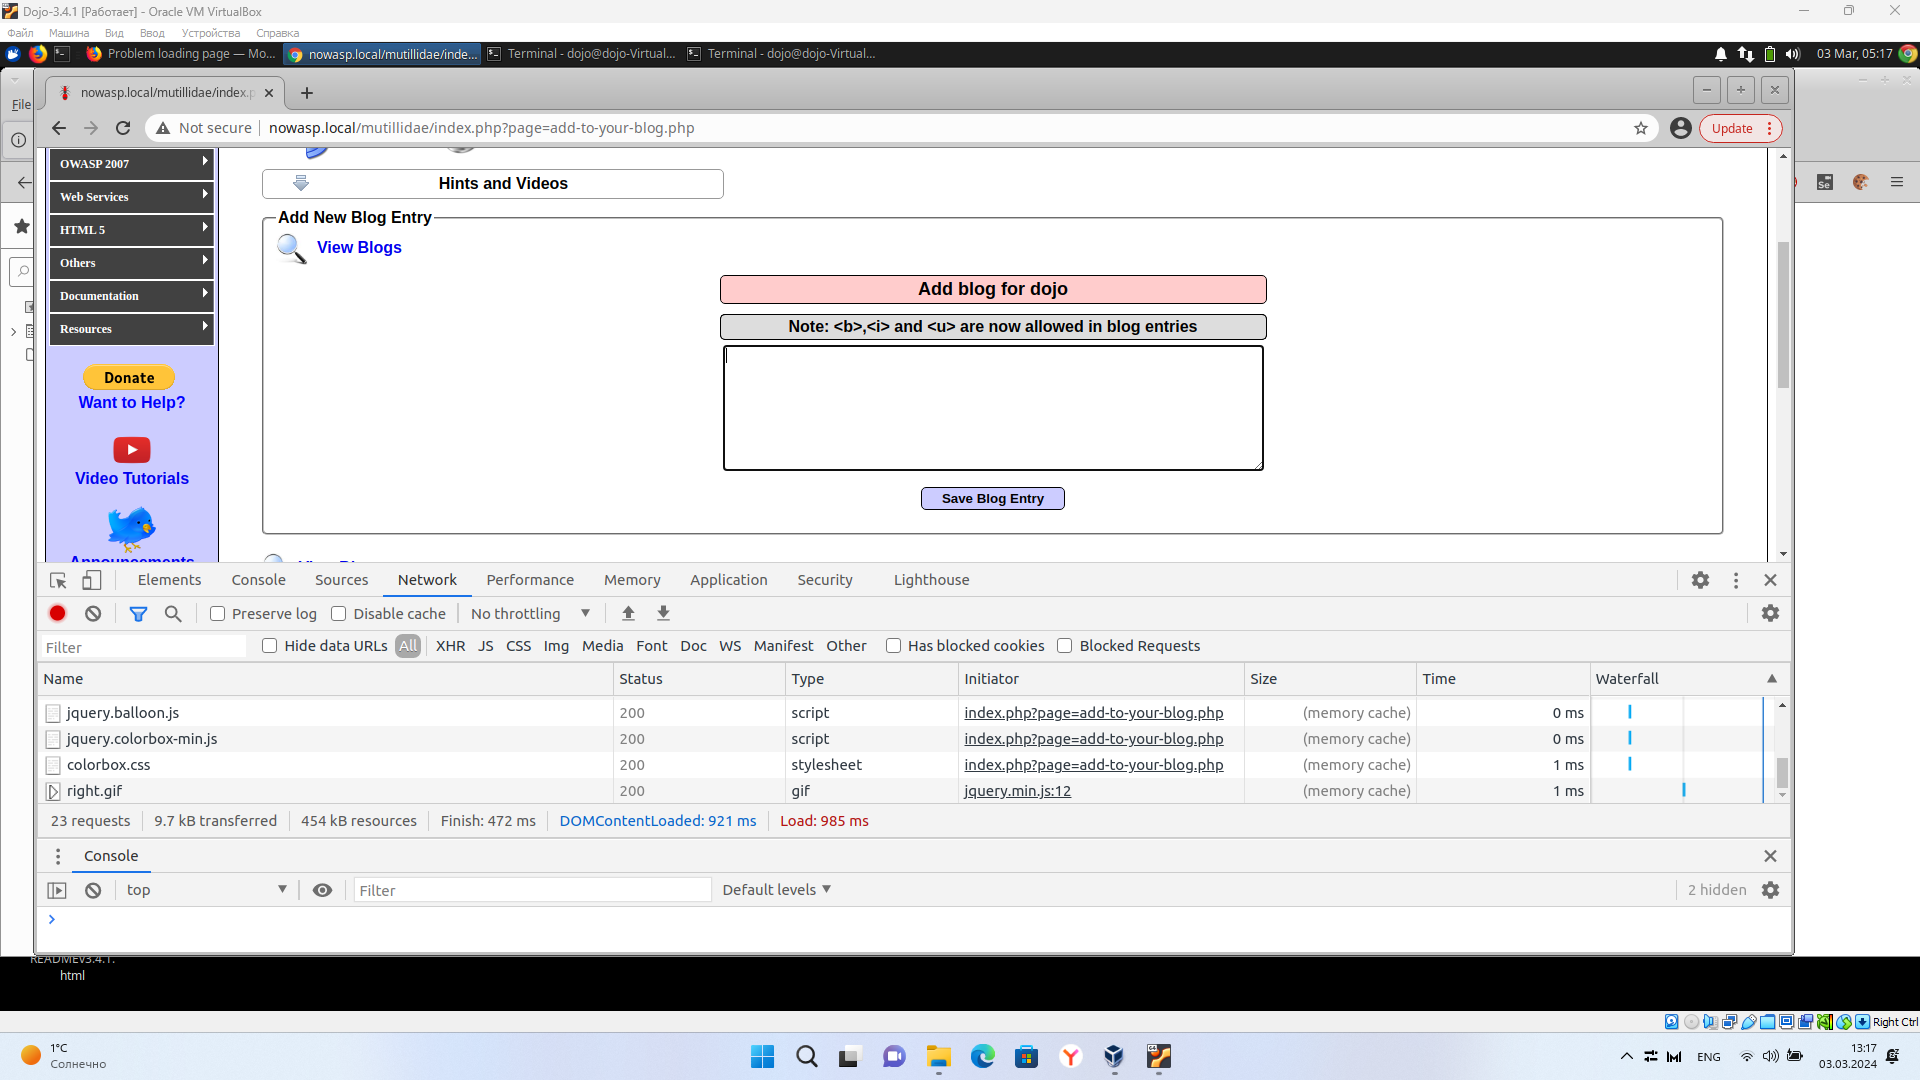
\includegraphics[width=\textwidth]{Screenshot_27}
    \caption{Новый пост создан}
  \end{figure}

  \begin{figure}[H]
    \centering
    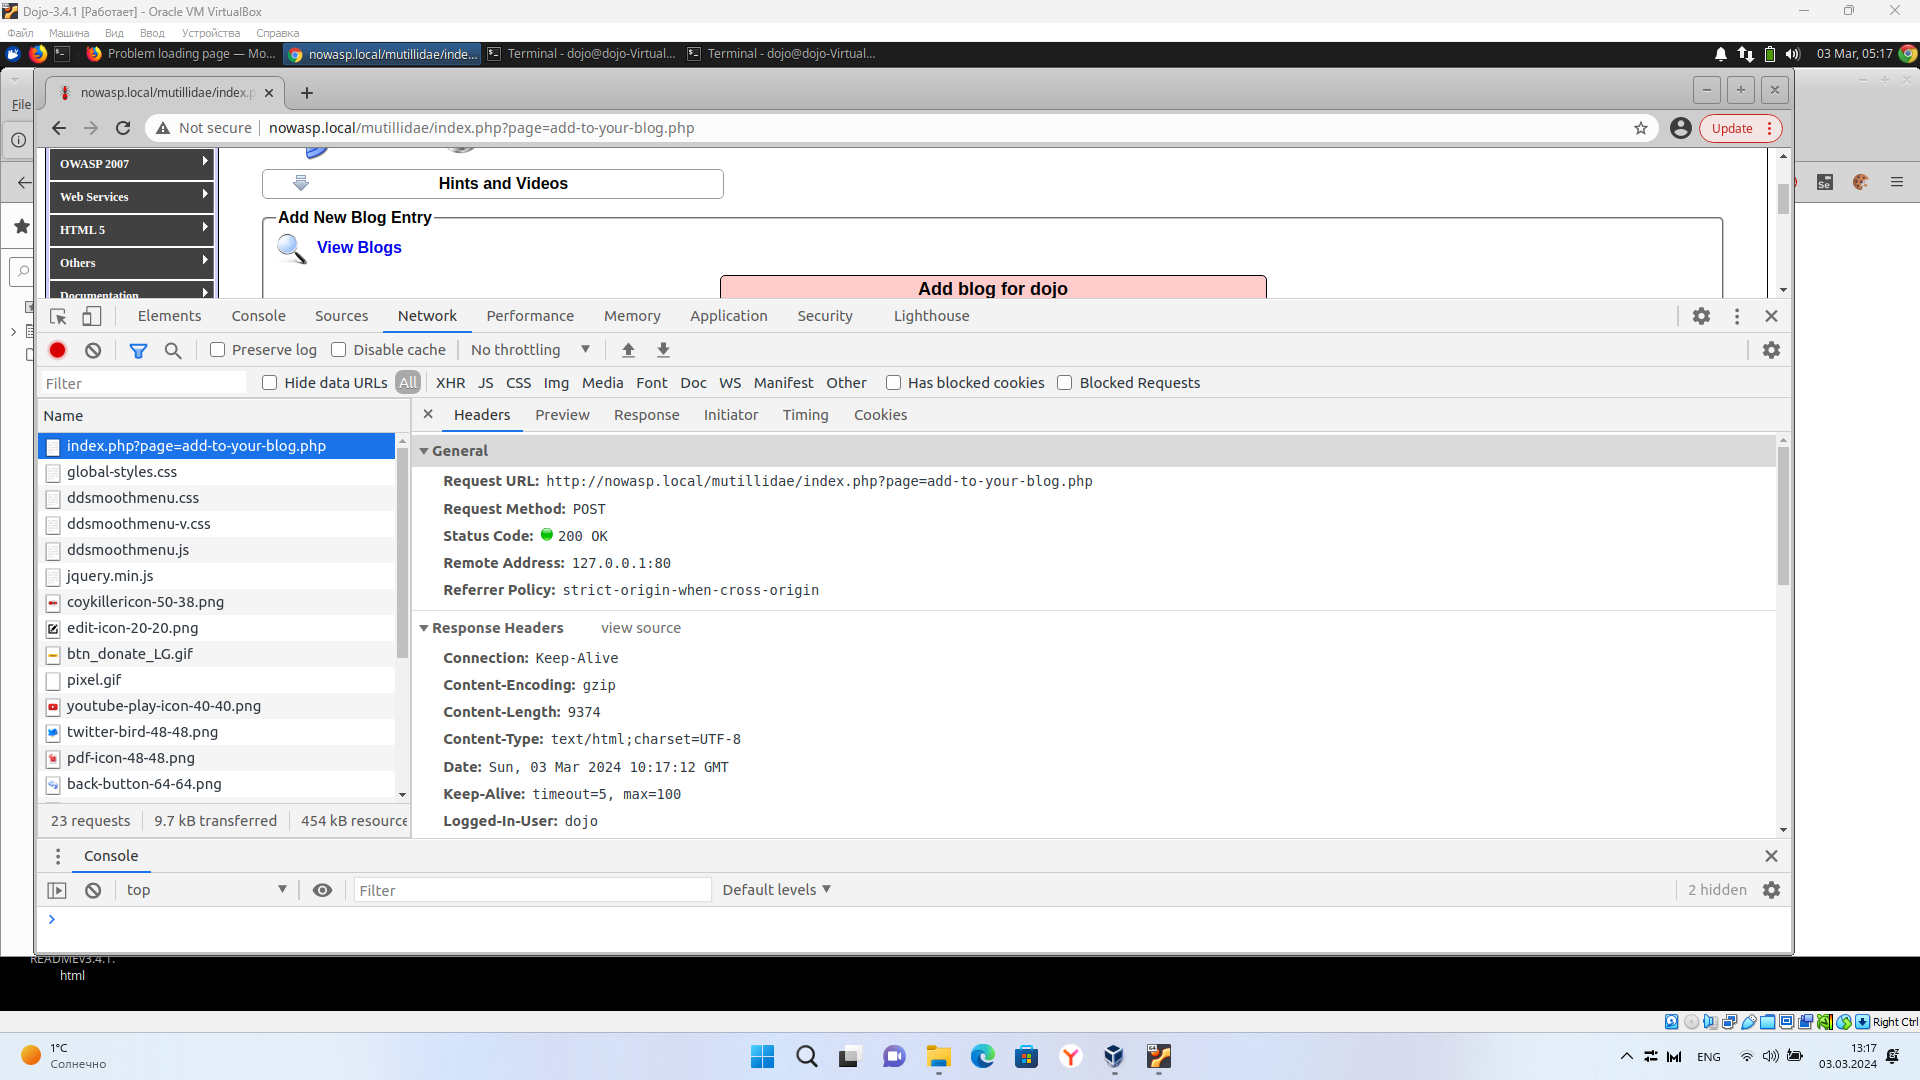
\includegraphics[width=\textwidth]{Screenshot_28}
    \caption{Открываем запрос на добавление новой записи}
  \end{figure}

  \begin{figure}[H]
    \centering
    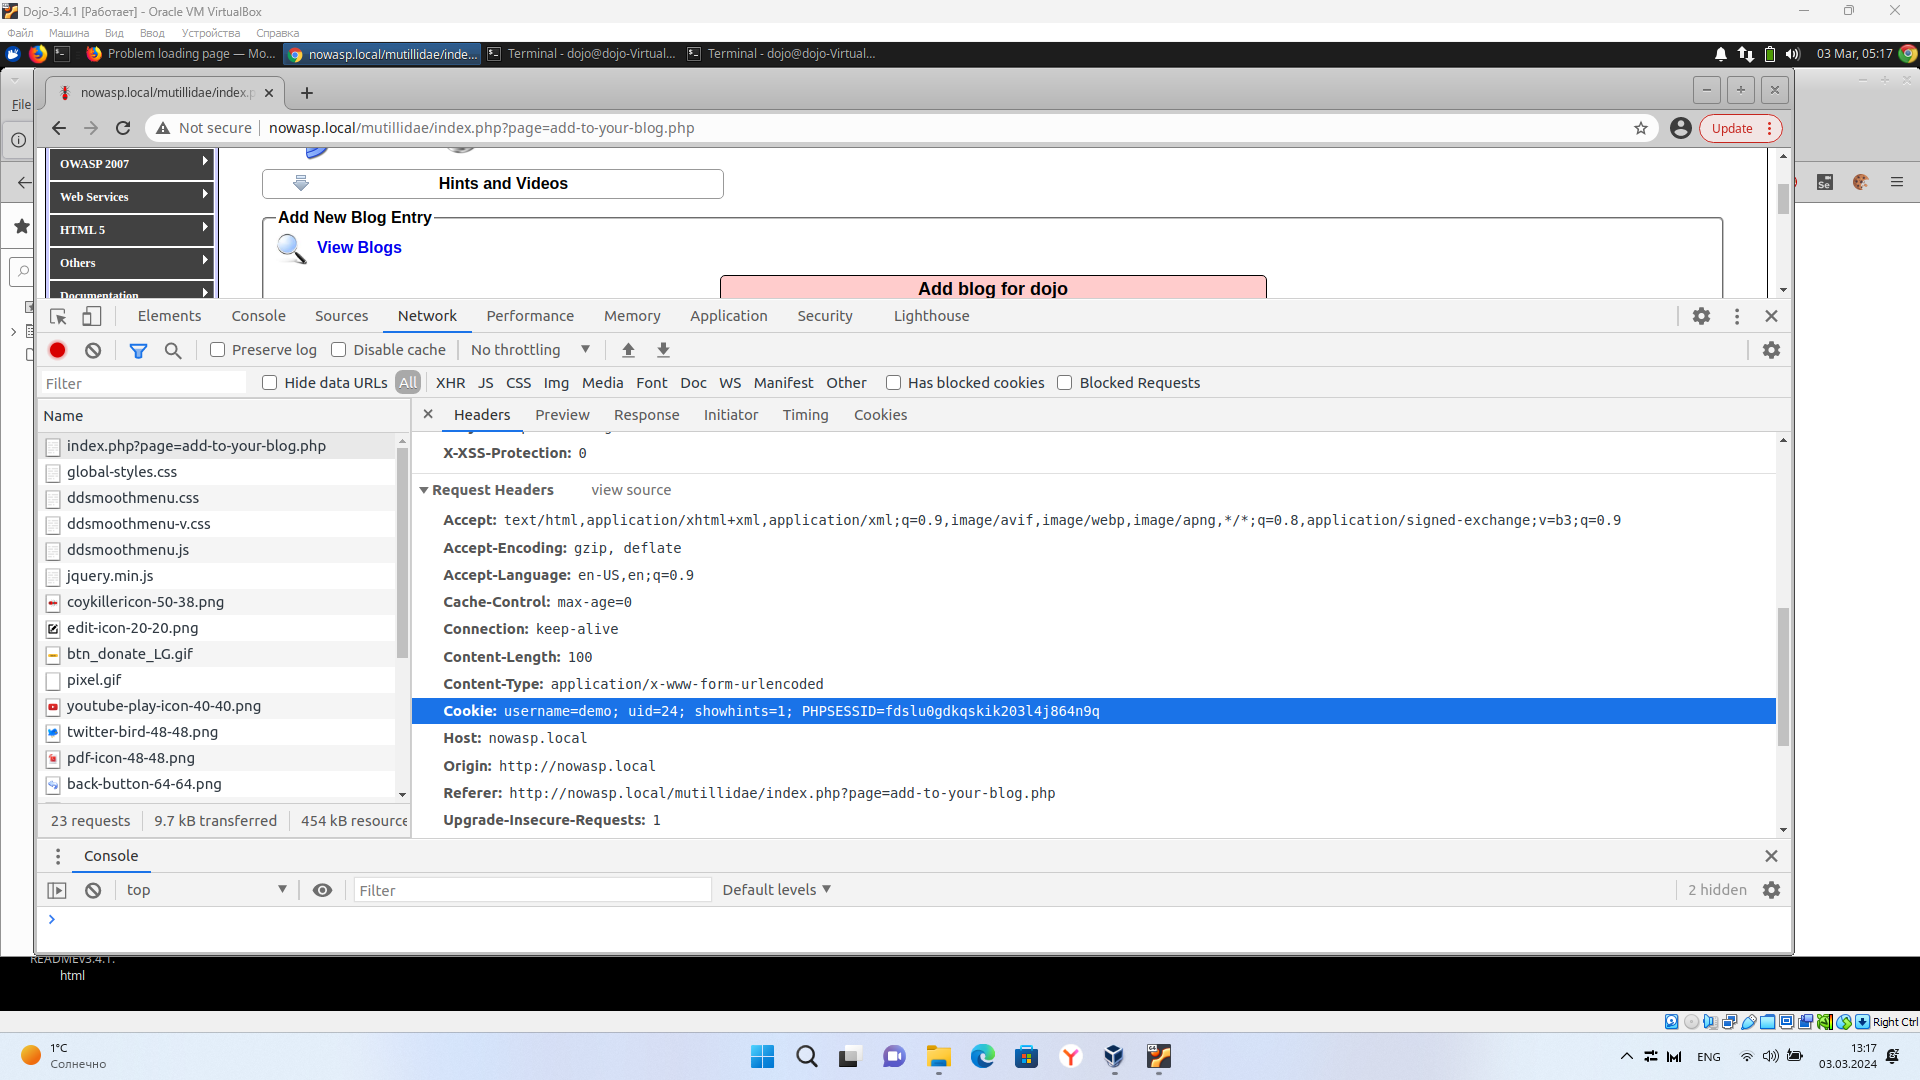
\includegraphics[width=\textwidth]{Screenshot_29}
    \caption{Смотрим, какие cookie отправляется вместе с запросом}
  \end{figure}

  \begin{figure}[H]
    \centering
    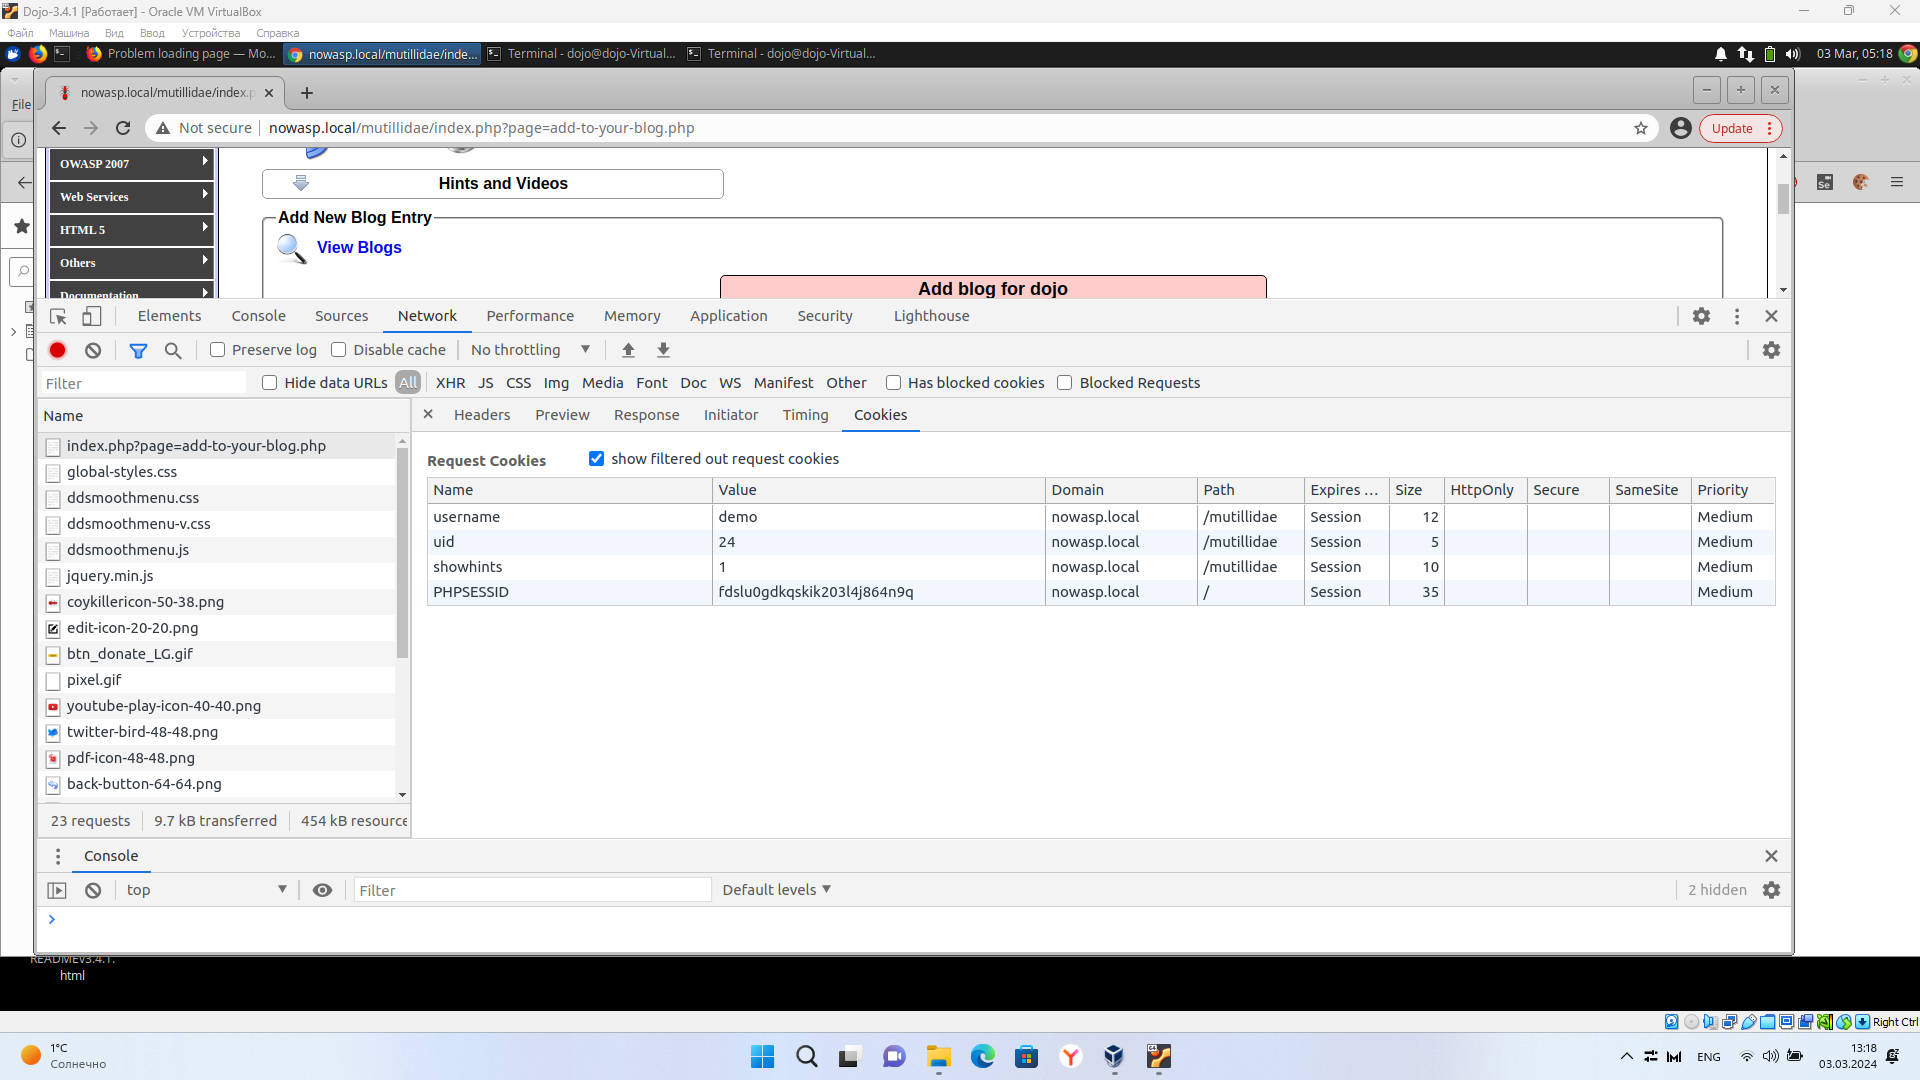
\includegraphics[width=\textwidth]{Screenshot_30}
    \caption{Те же cookie, но в другом отображении}
  \end{figure}

  \begin{figure}[H]
    \centering
    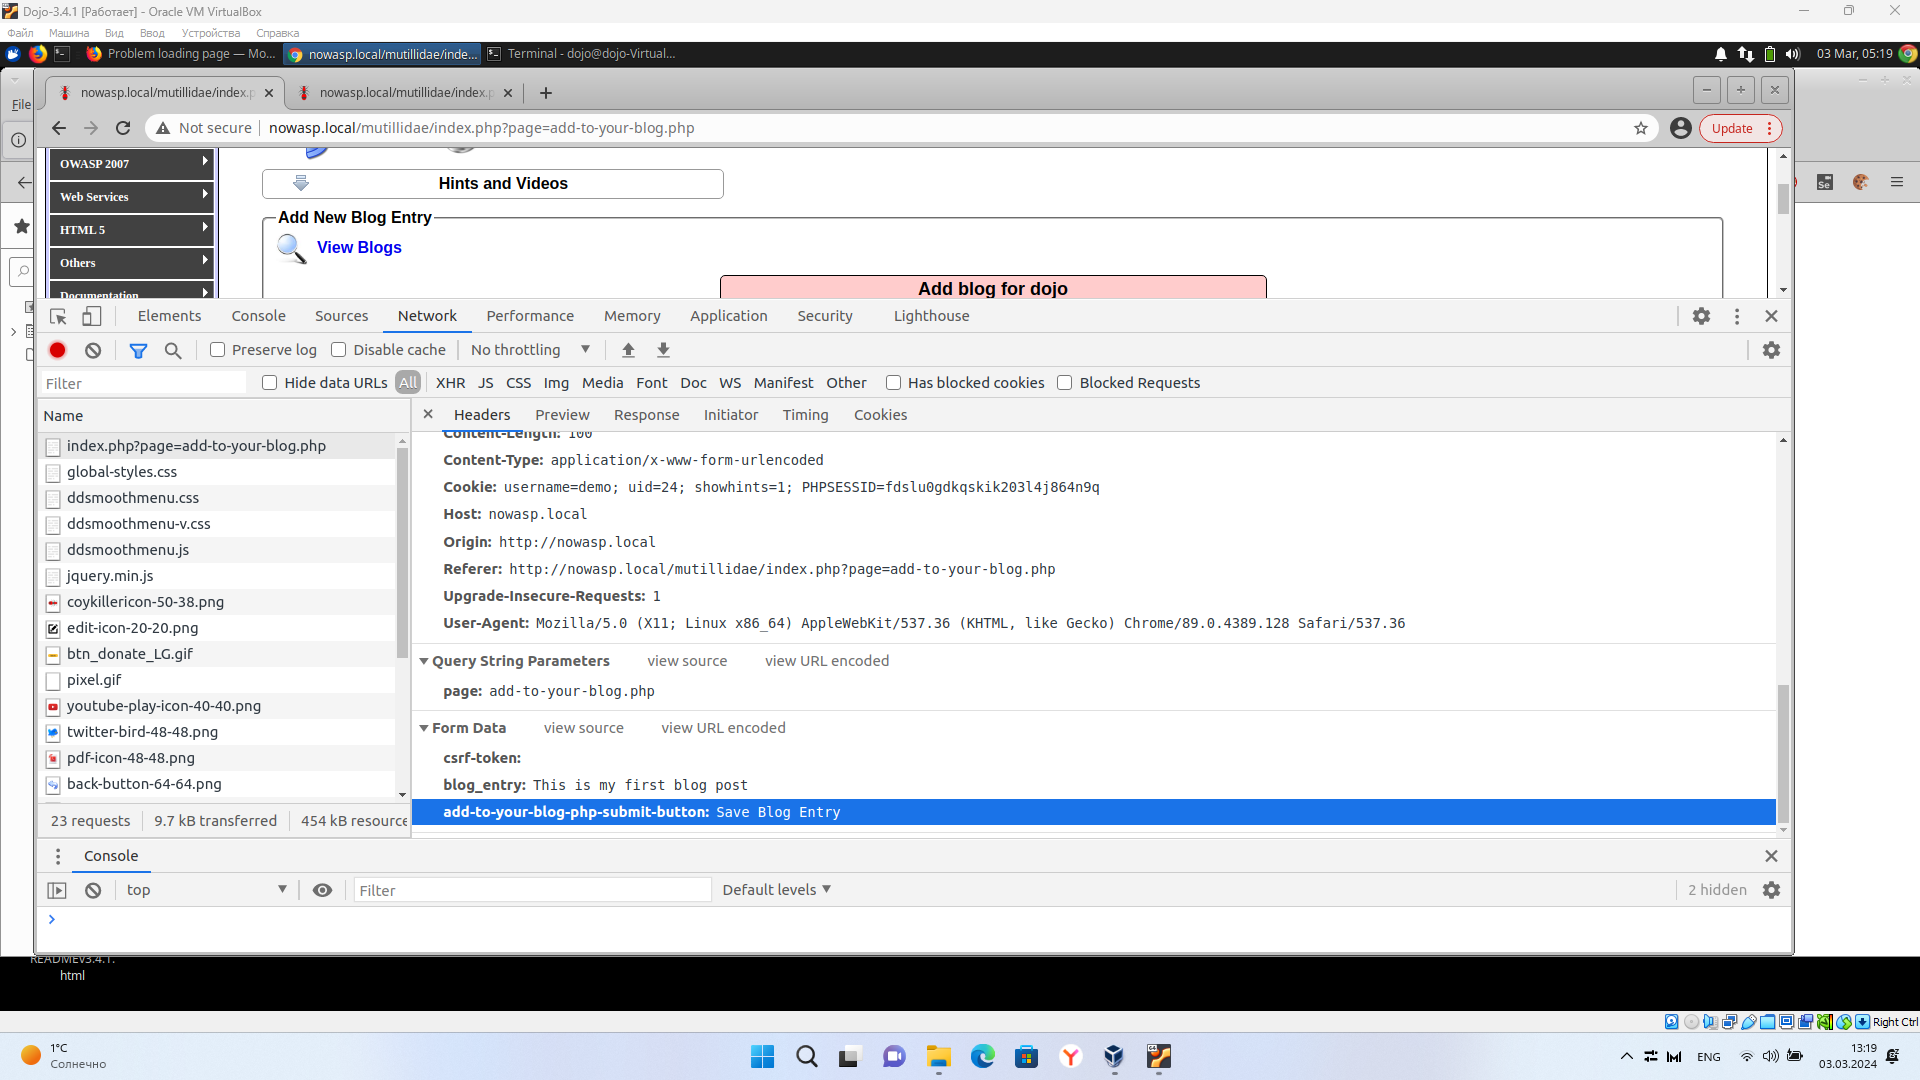
\includegraphics[width=\textwidth]{Screenshot_31}
    \caption{Смотрим параметры запроса}
  \end{figure}

  Что стало понятно в ходе анализа запроса: это POST запрос на атакуемую страницу с указанием параметра page (в значение
  add-to-your-blog). Вместе с этим запросом передается cookie сессии (PHPSESSID) и текст нового поста (как form data параметры).

  \begin{figure}[H]
    \centering
    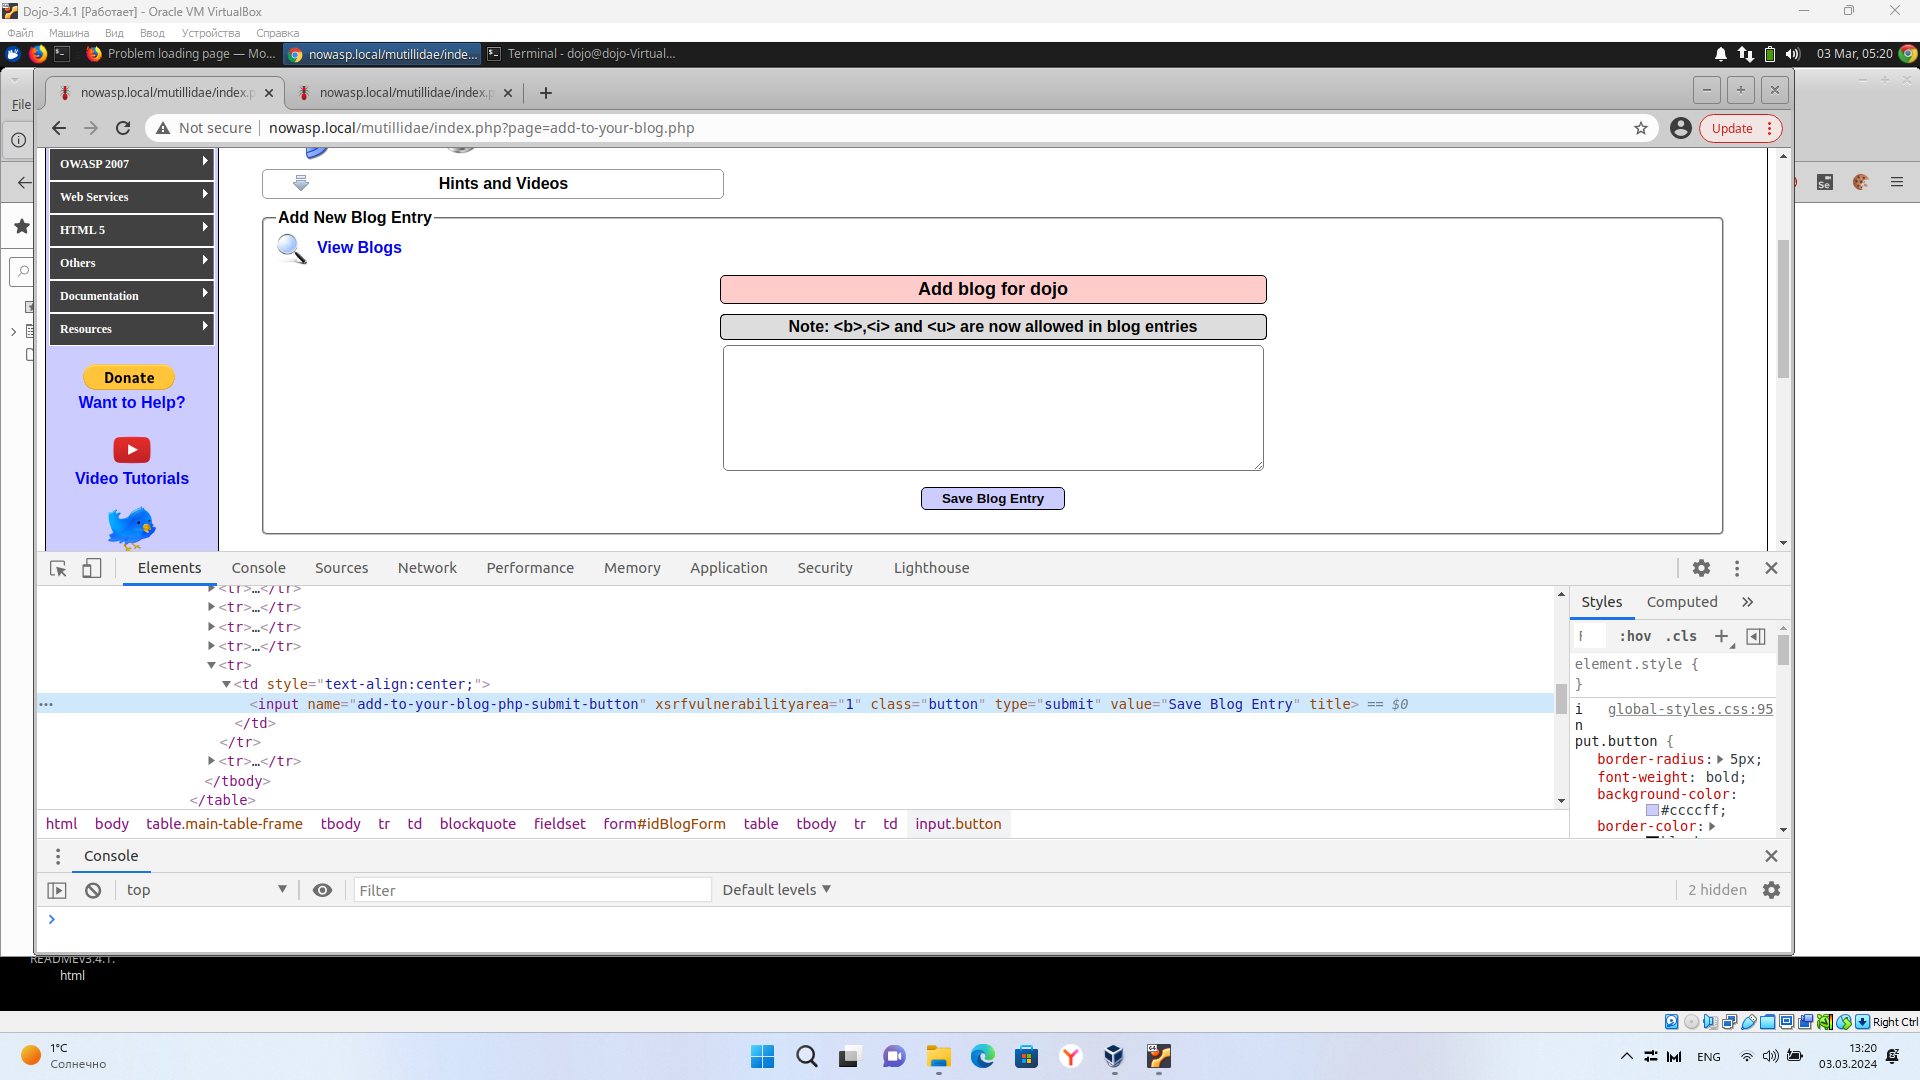
\includegraphics[width=\textwidth]{Screenshot_32}
    \caption{Смотрим код страницы - это обычная html форма}
  \end{figure}

  \begin{figure}[H]
    \centering
    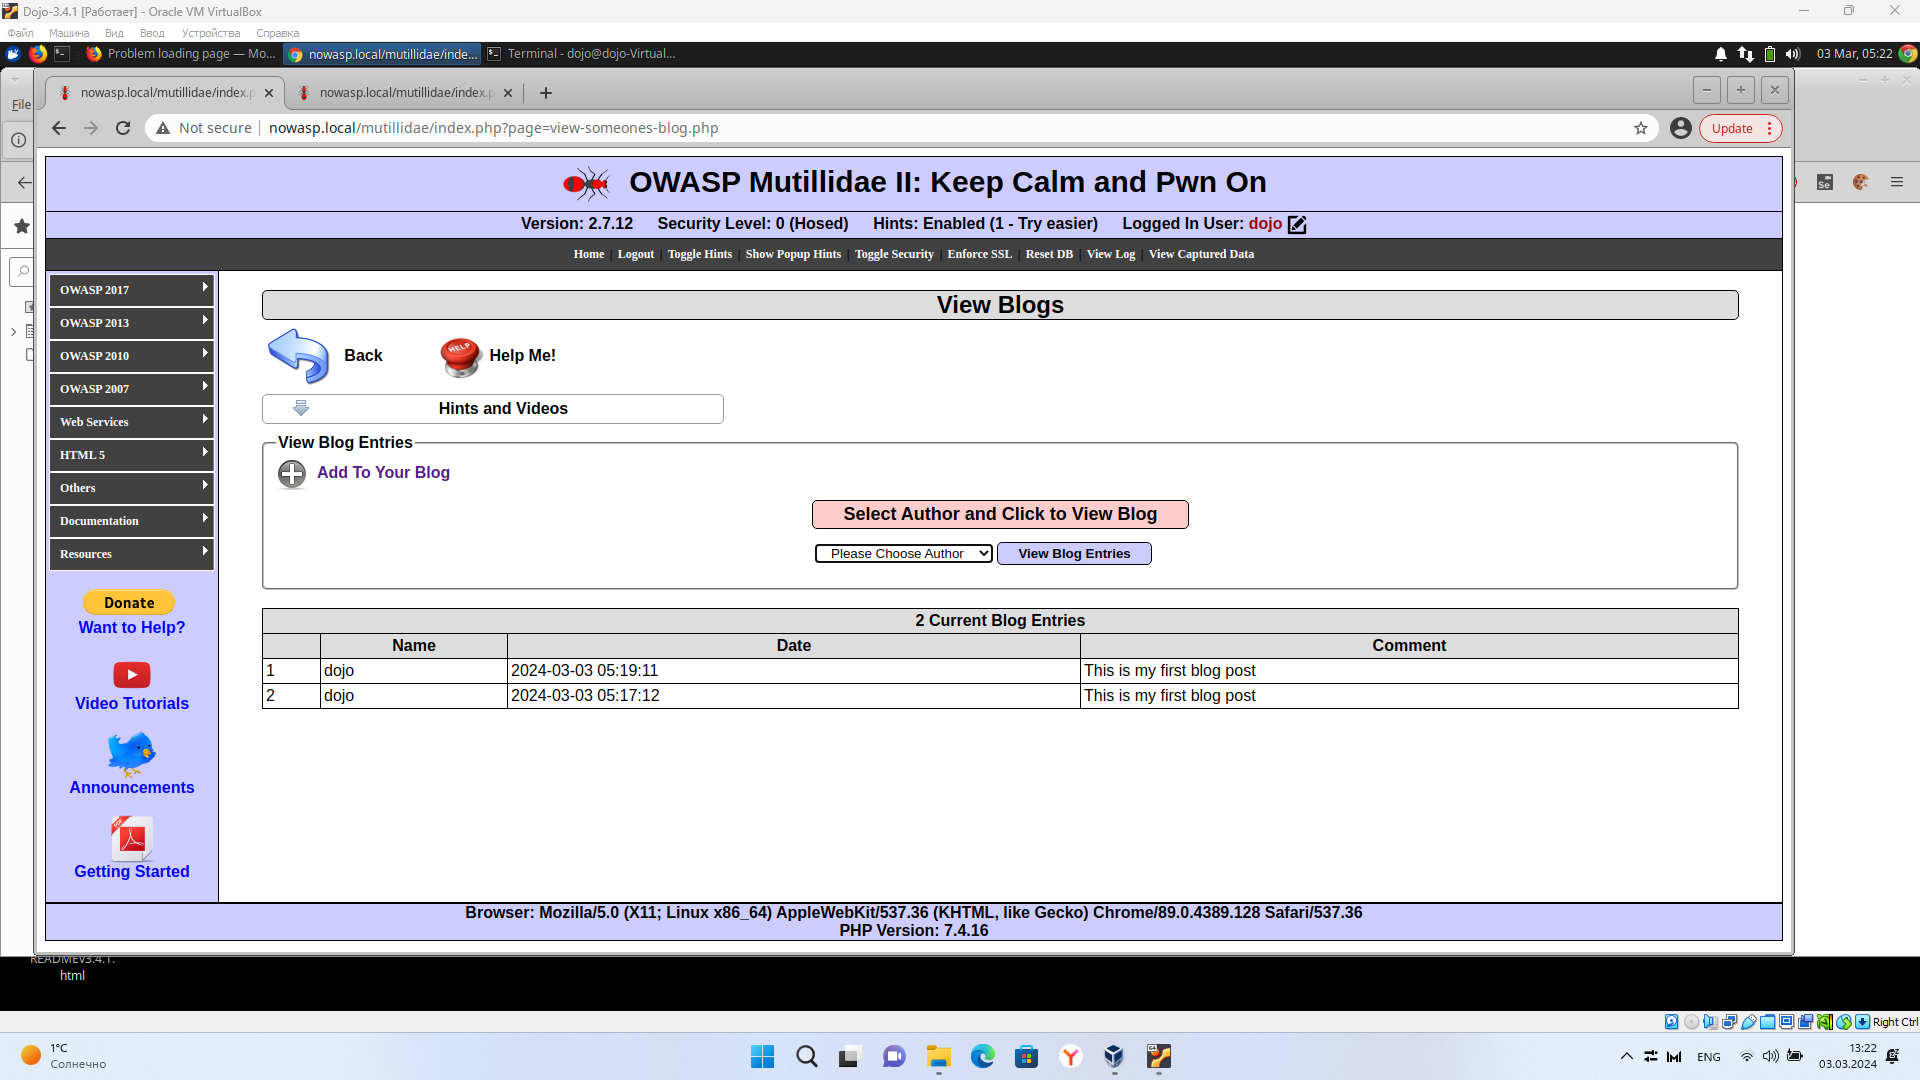
\includegraphics[width=\textwidth]{Screenshot_33}
    \caption{В списке постов мы видем нашу публикацию}
  \end{figure}

  \subsubsection{Проводим атаку}

  \begin{figure}[H]
    \centering
    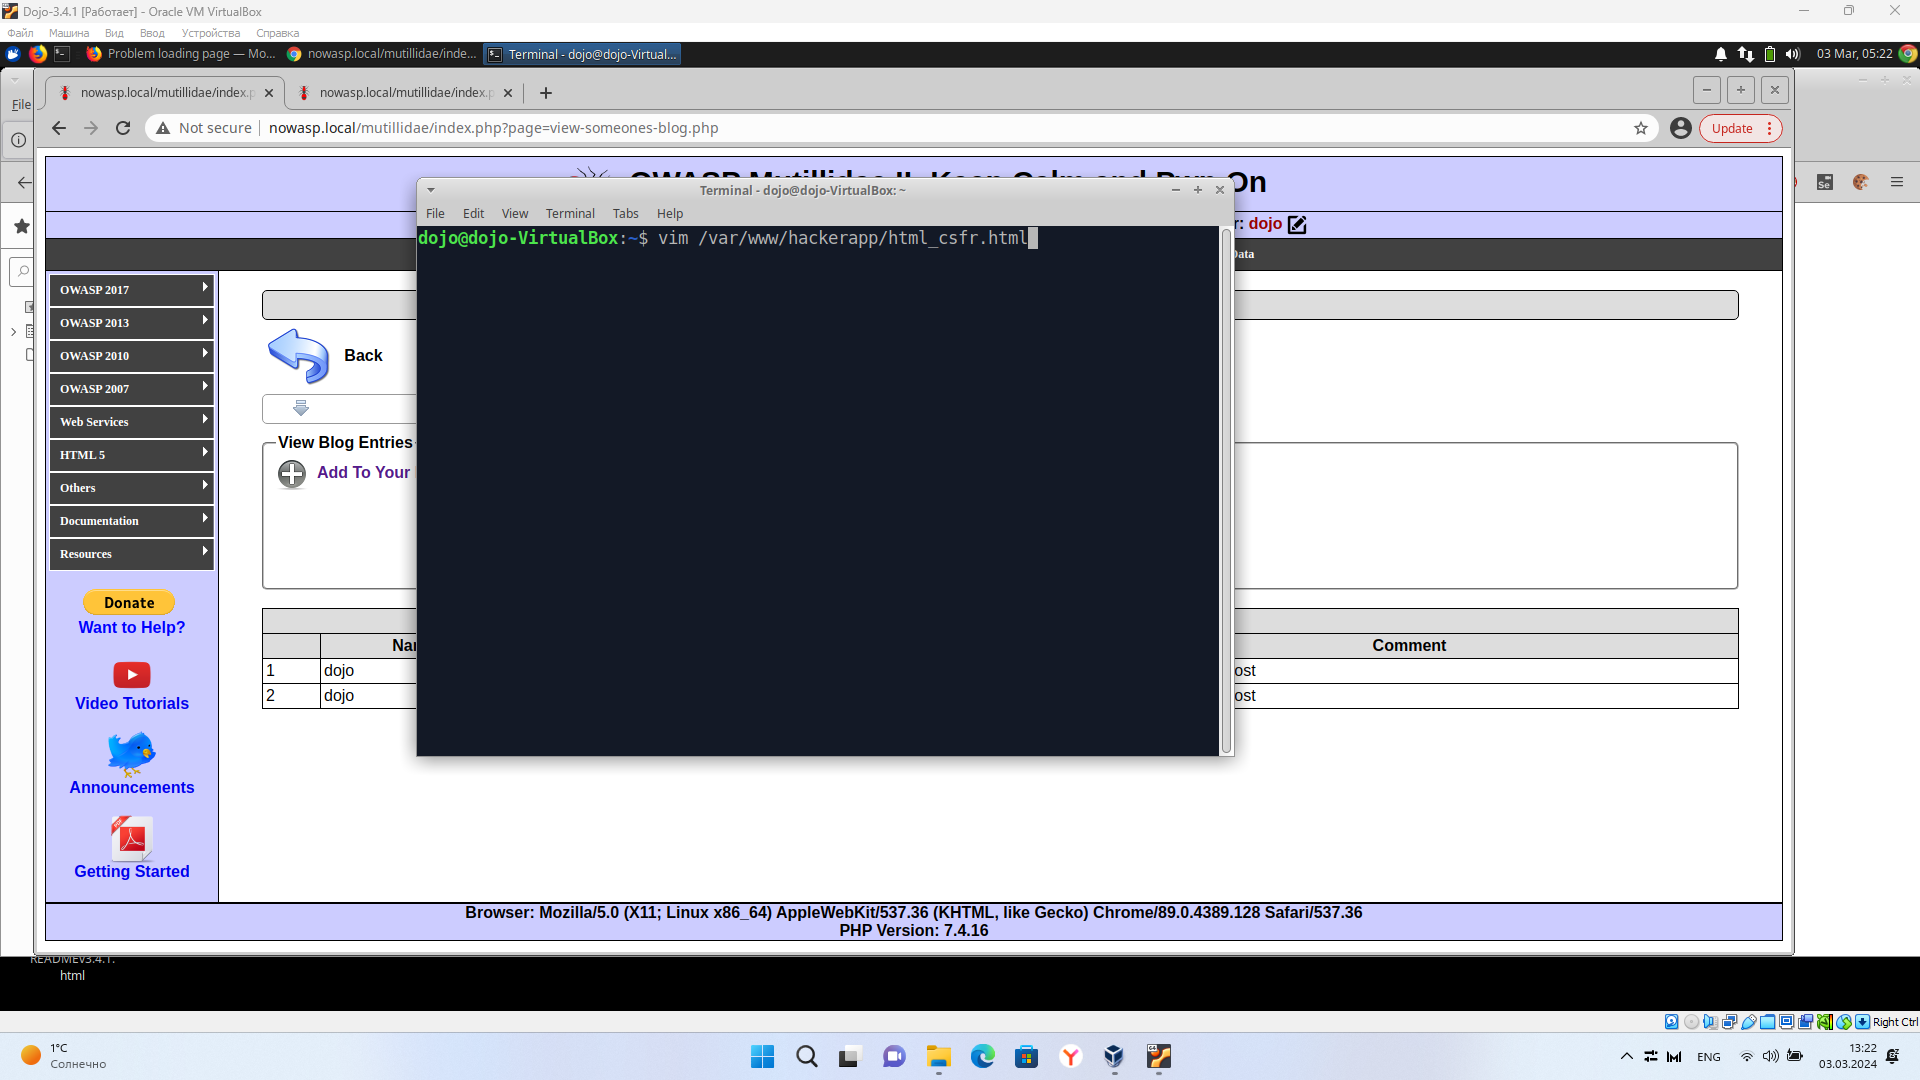
\includegraphics[width=\textwidth]{Screenshot_34}
    \caption{Создаем html страничку сайта злоумышленника}
  \end{figure}

  \begin{figure}[H]
    \centering
    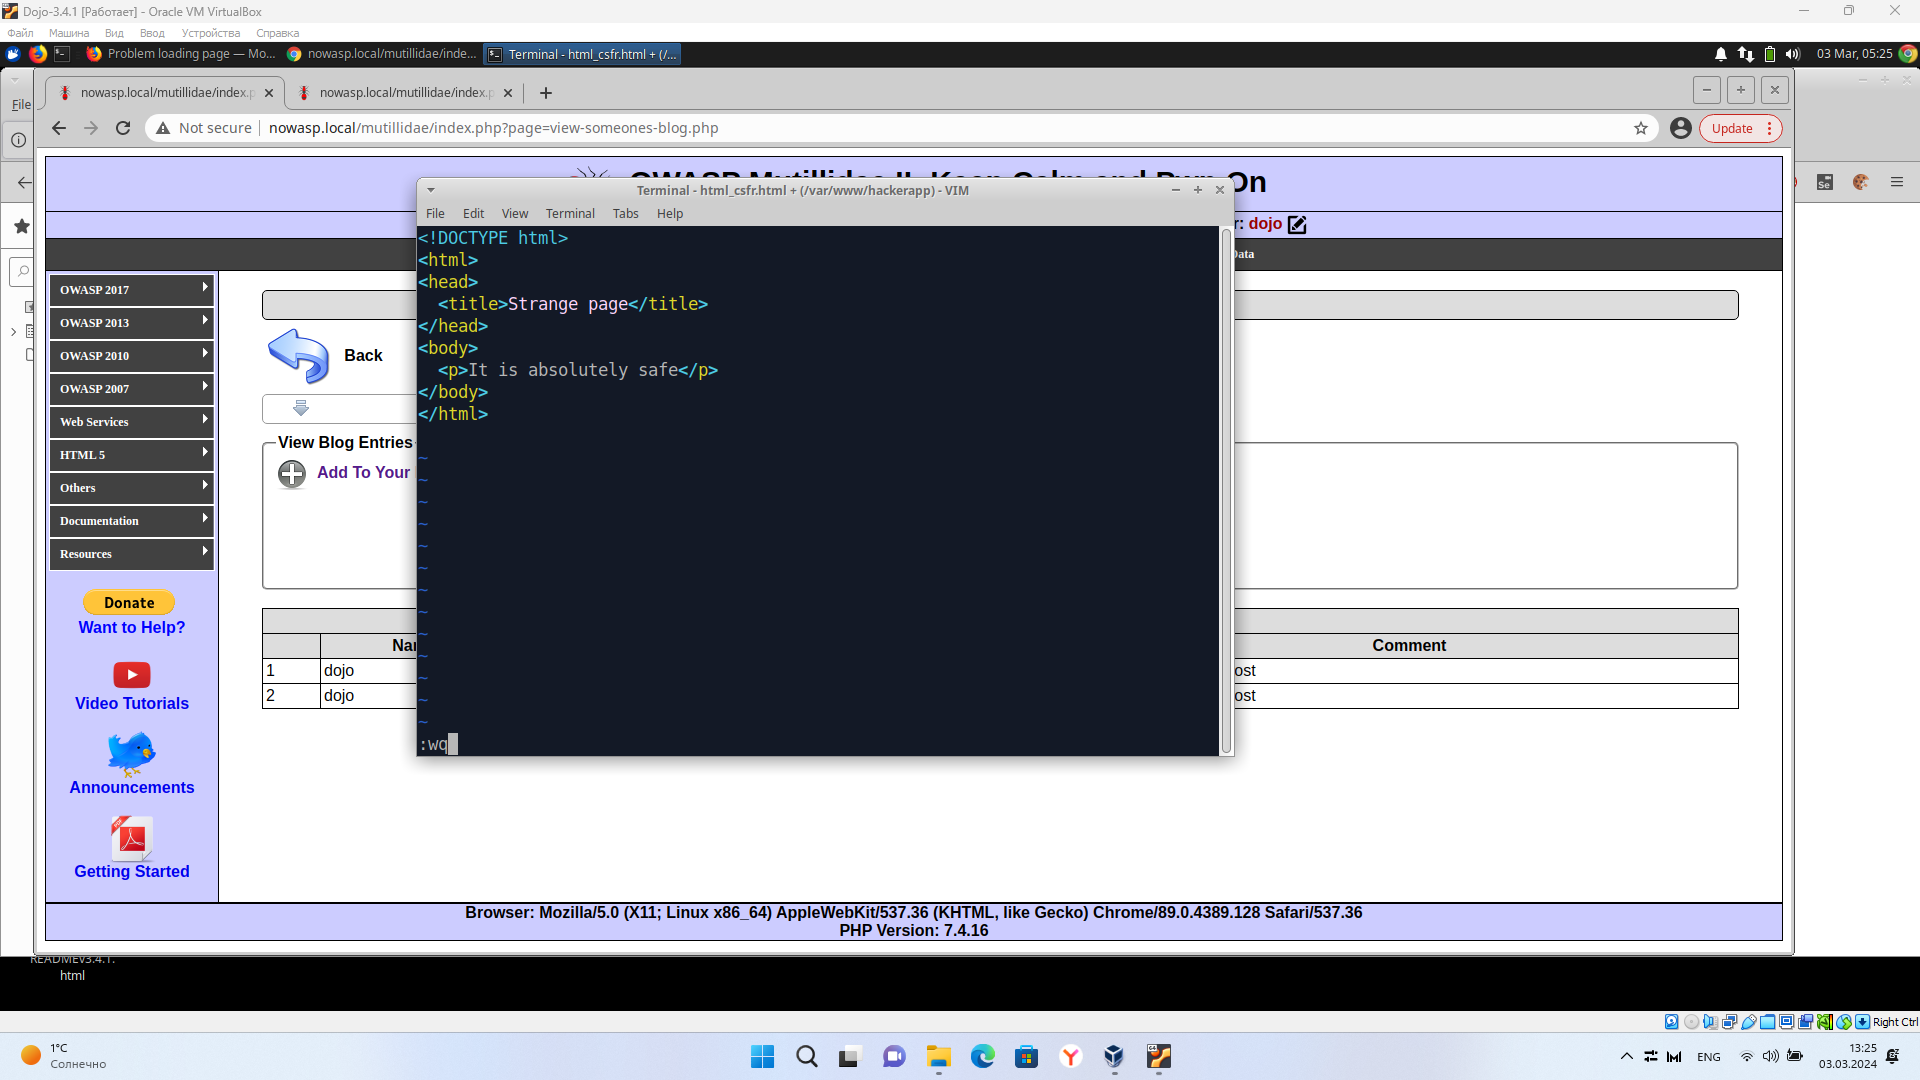
\includegraphics[width=\textwidth]{Screenshot_35}
    \caption{Создаем простую html разметку для проверки работоспособности}
  \end{figure}

  \begin{figure}[H]
    \centering
    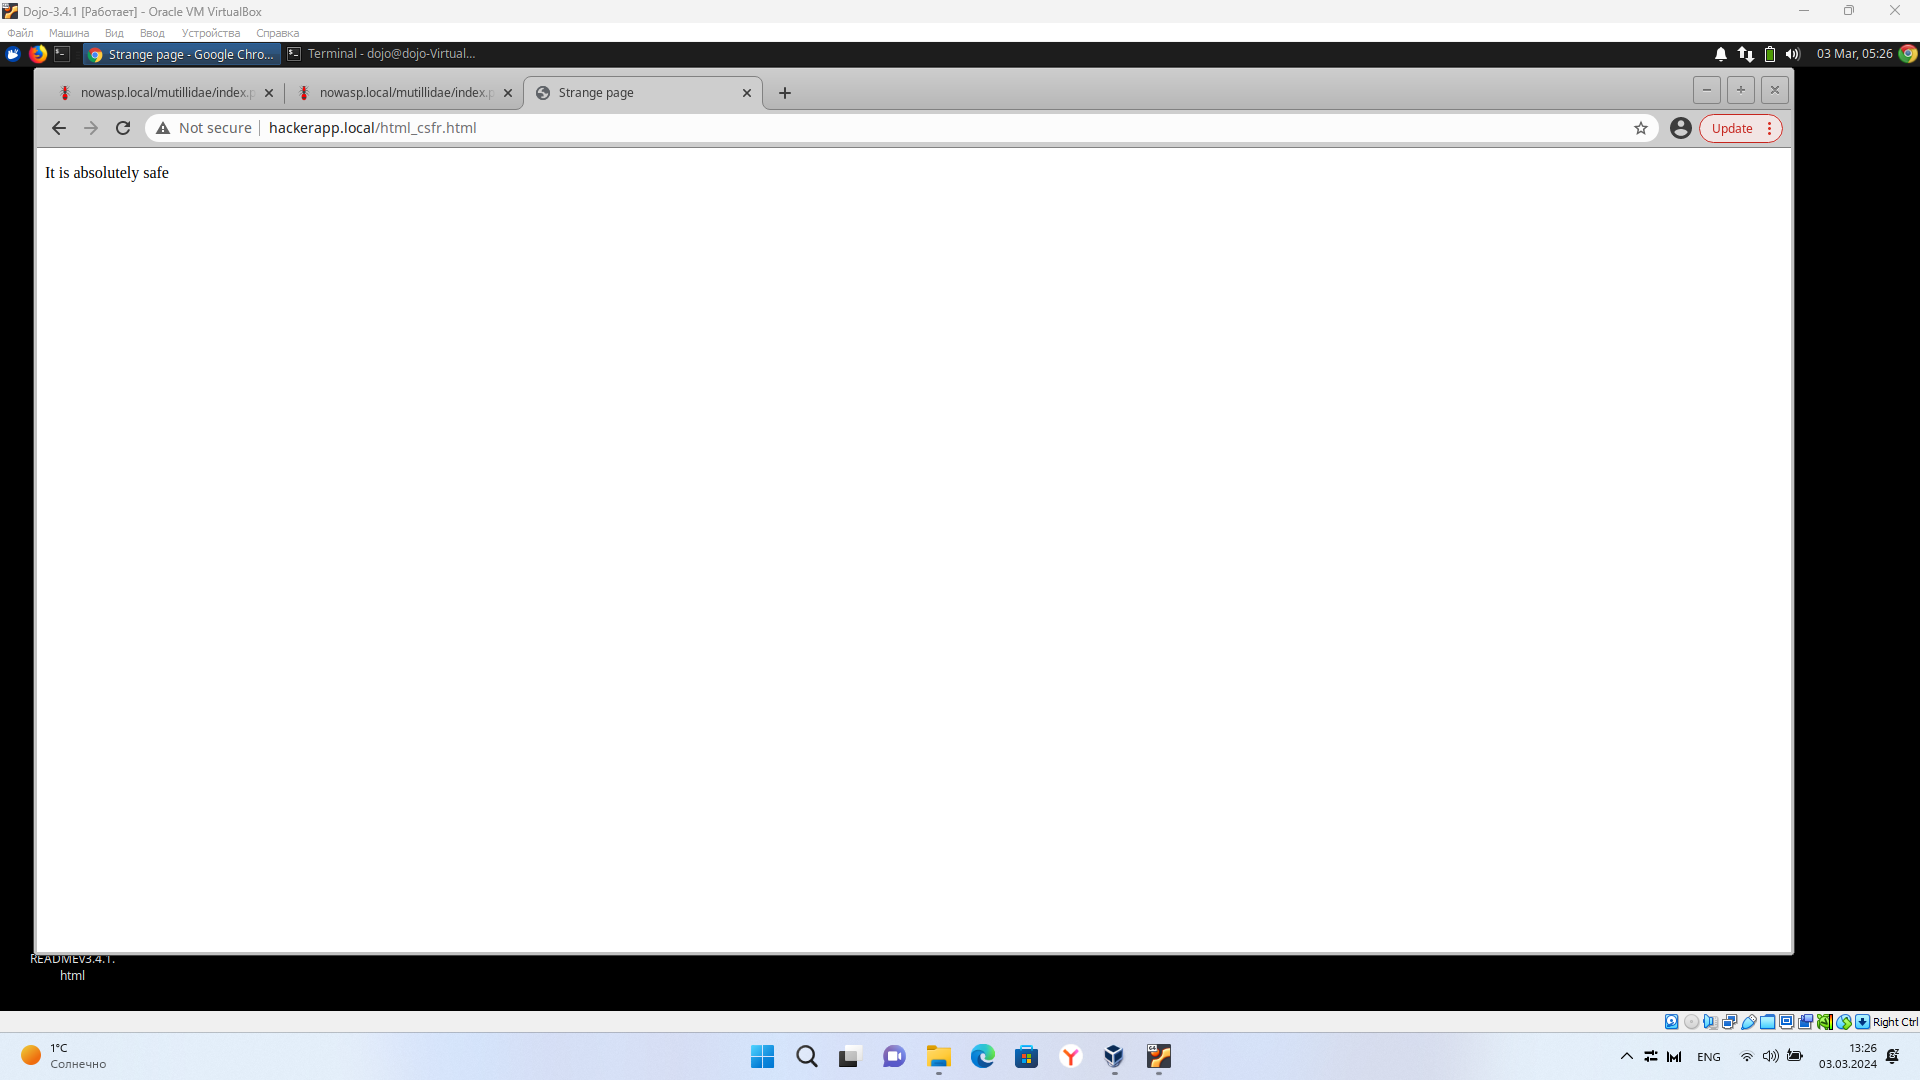
\includegraphics[width=\textwidth]{Screenshot_36}
    \caption{Открываем созданную страницу через браузер}
  \end{figure}

  \begin{figure}[H]
    \centering
    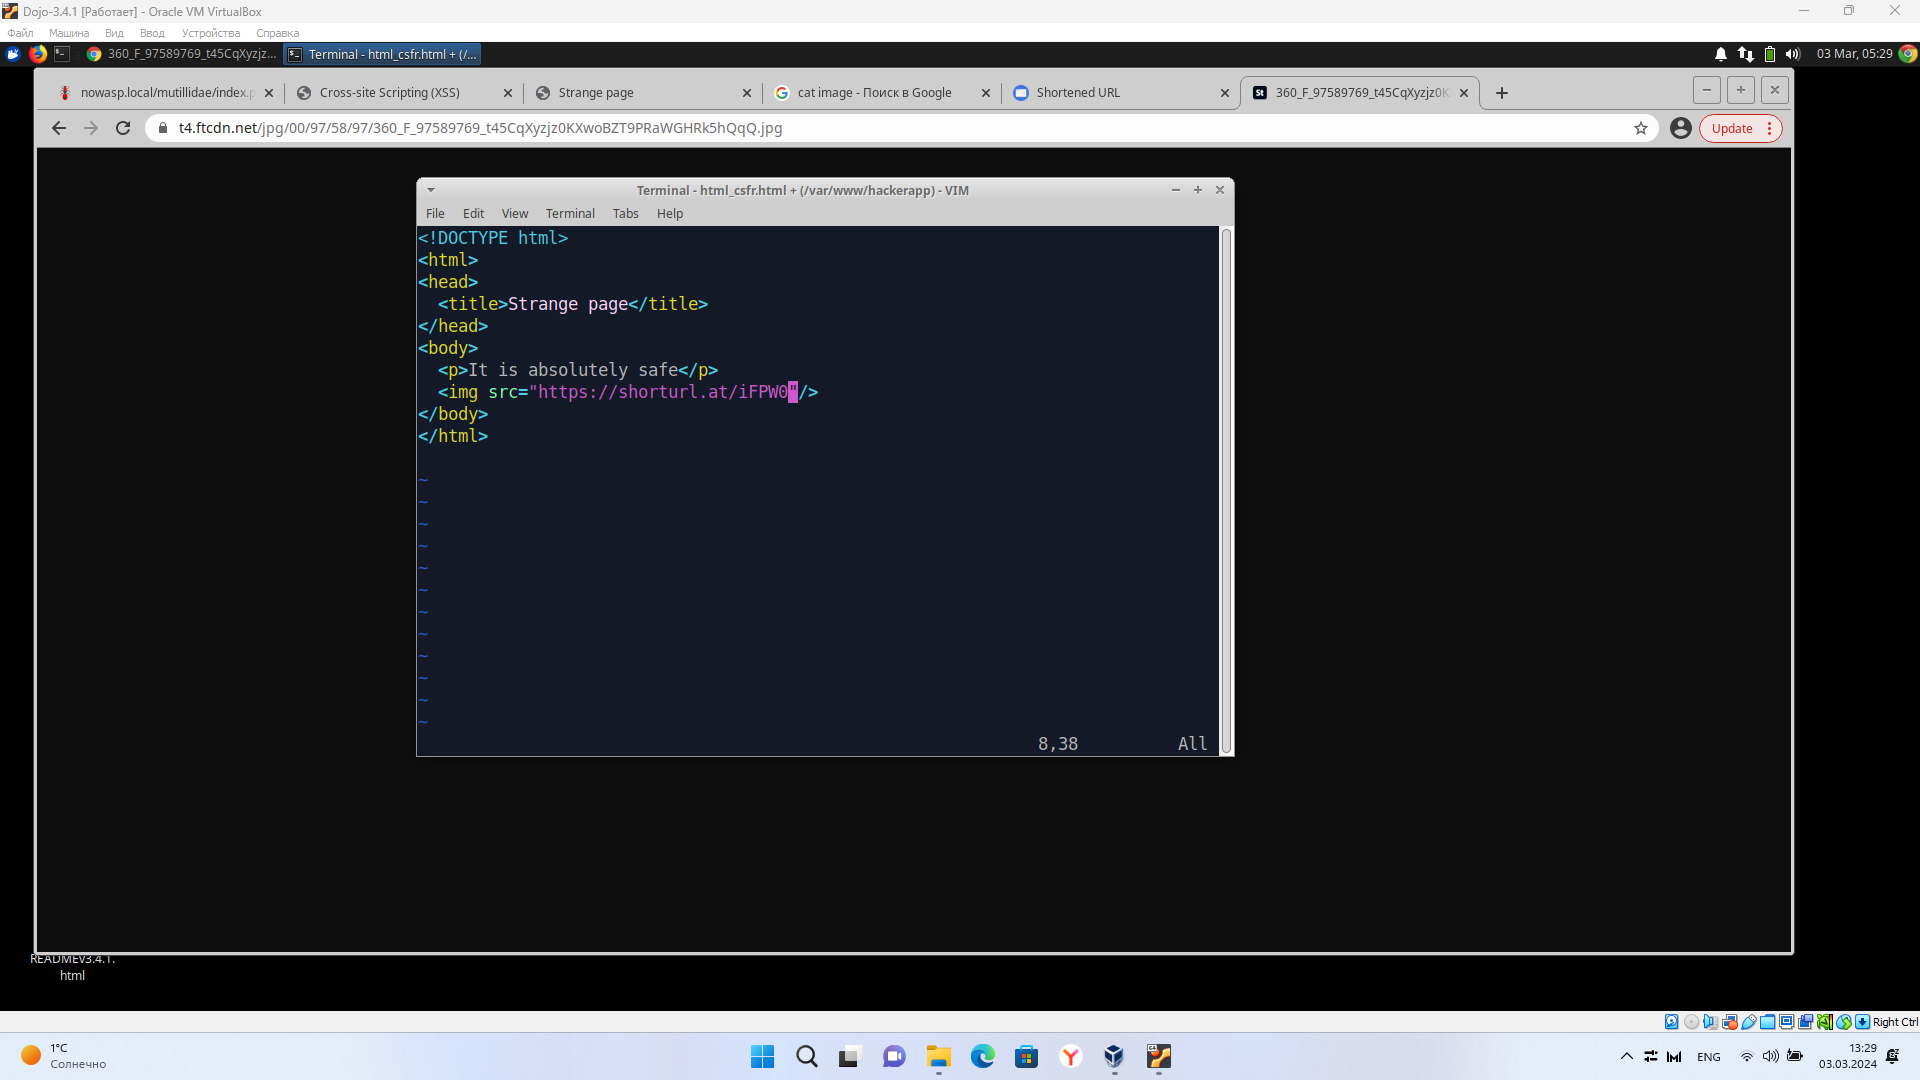
\includegraphics[width=\textwidth]{Screenshot_37}
    \caption{Вставляем на страницу картинку с пока безопасным контентом}
  \end{figure}

  \begin{figure}[H]
    \centering
    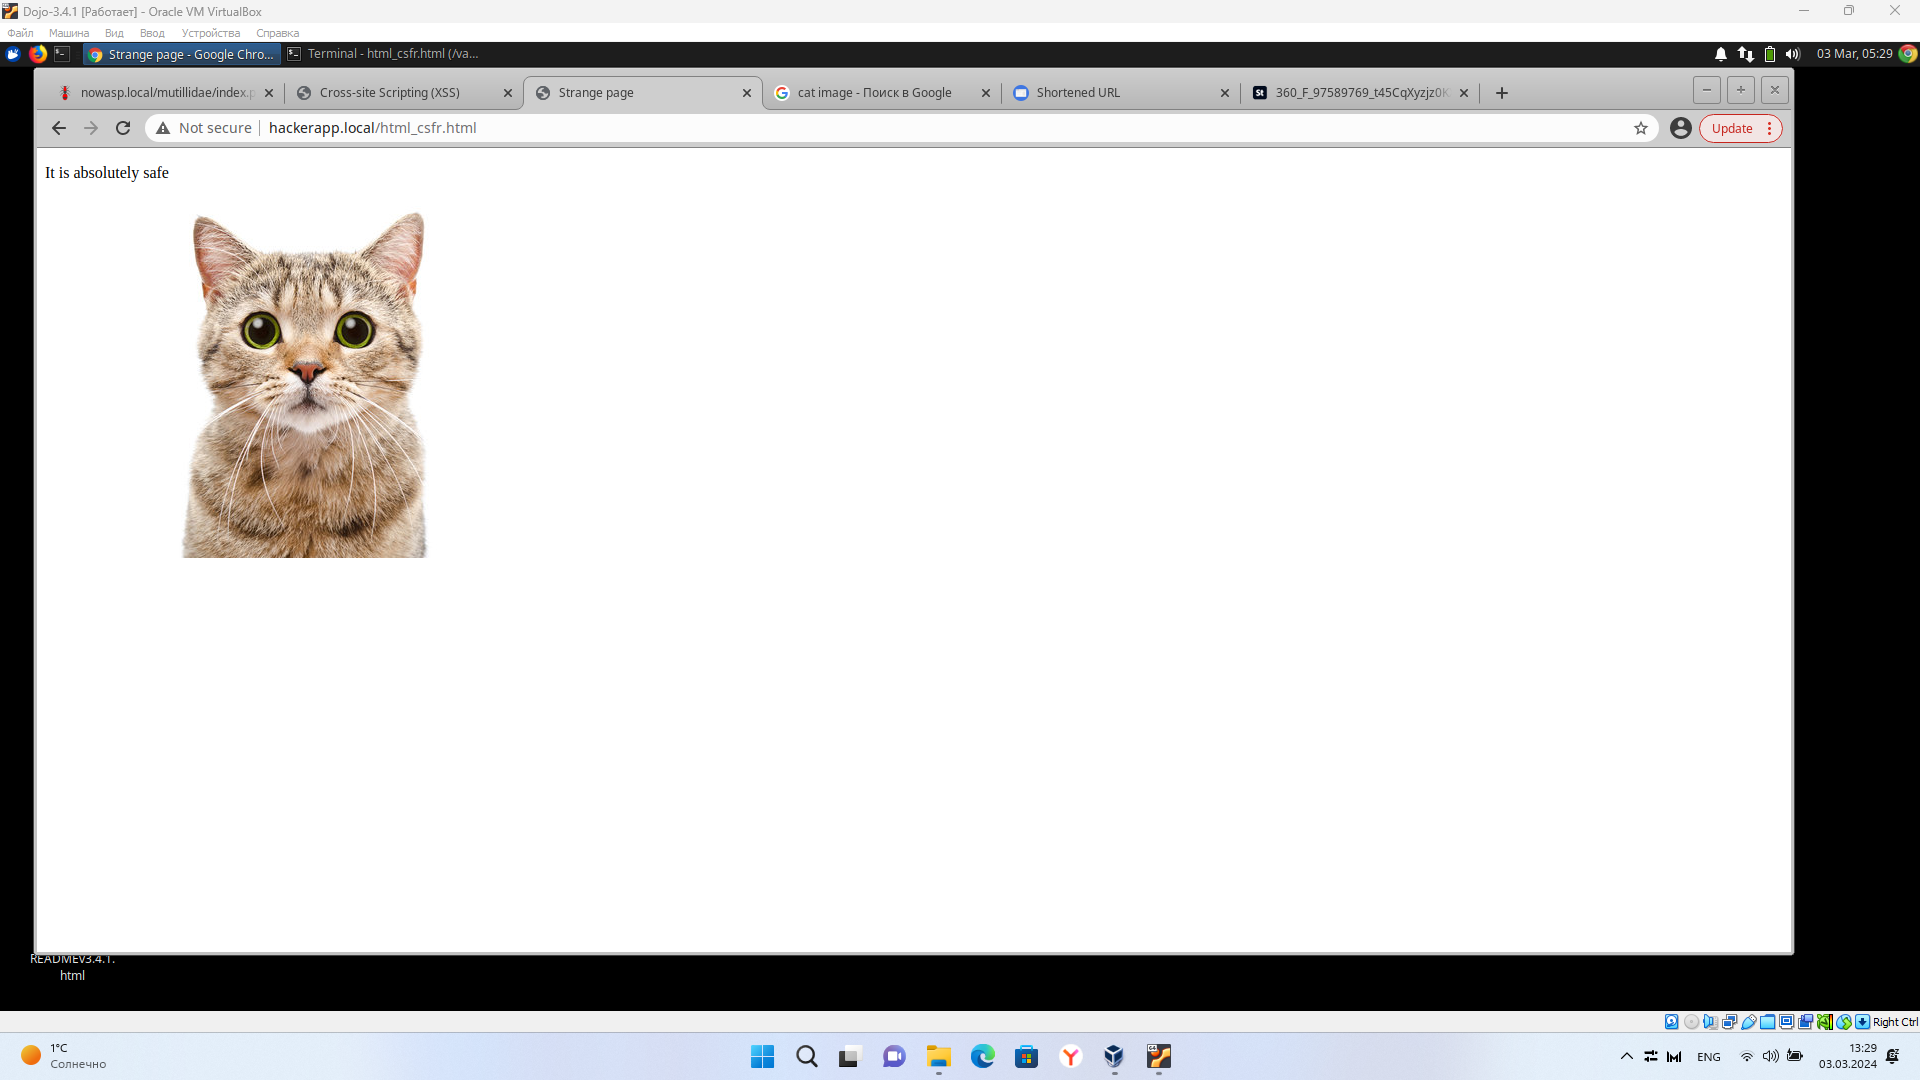
\includegraphics[width=\textwidth]{Screenshot_38}
    \caption{Видим картинку котика}
  \end{figure}

  \begin{figure}[H]
    \centering
    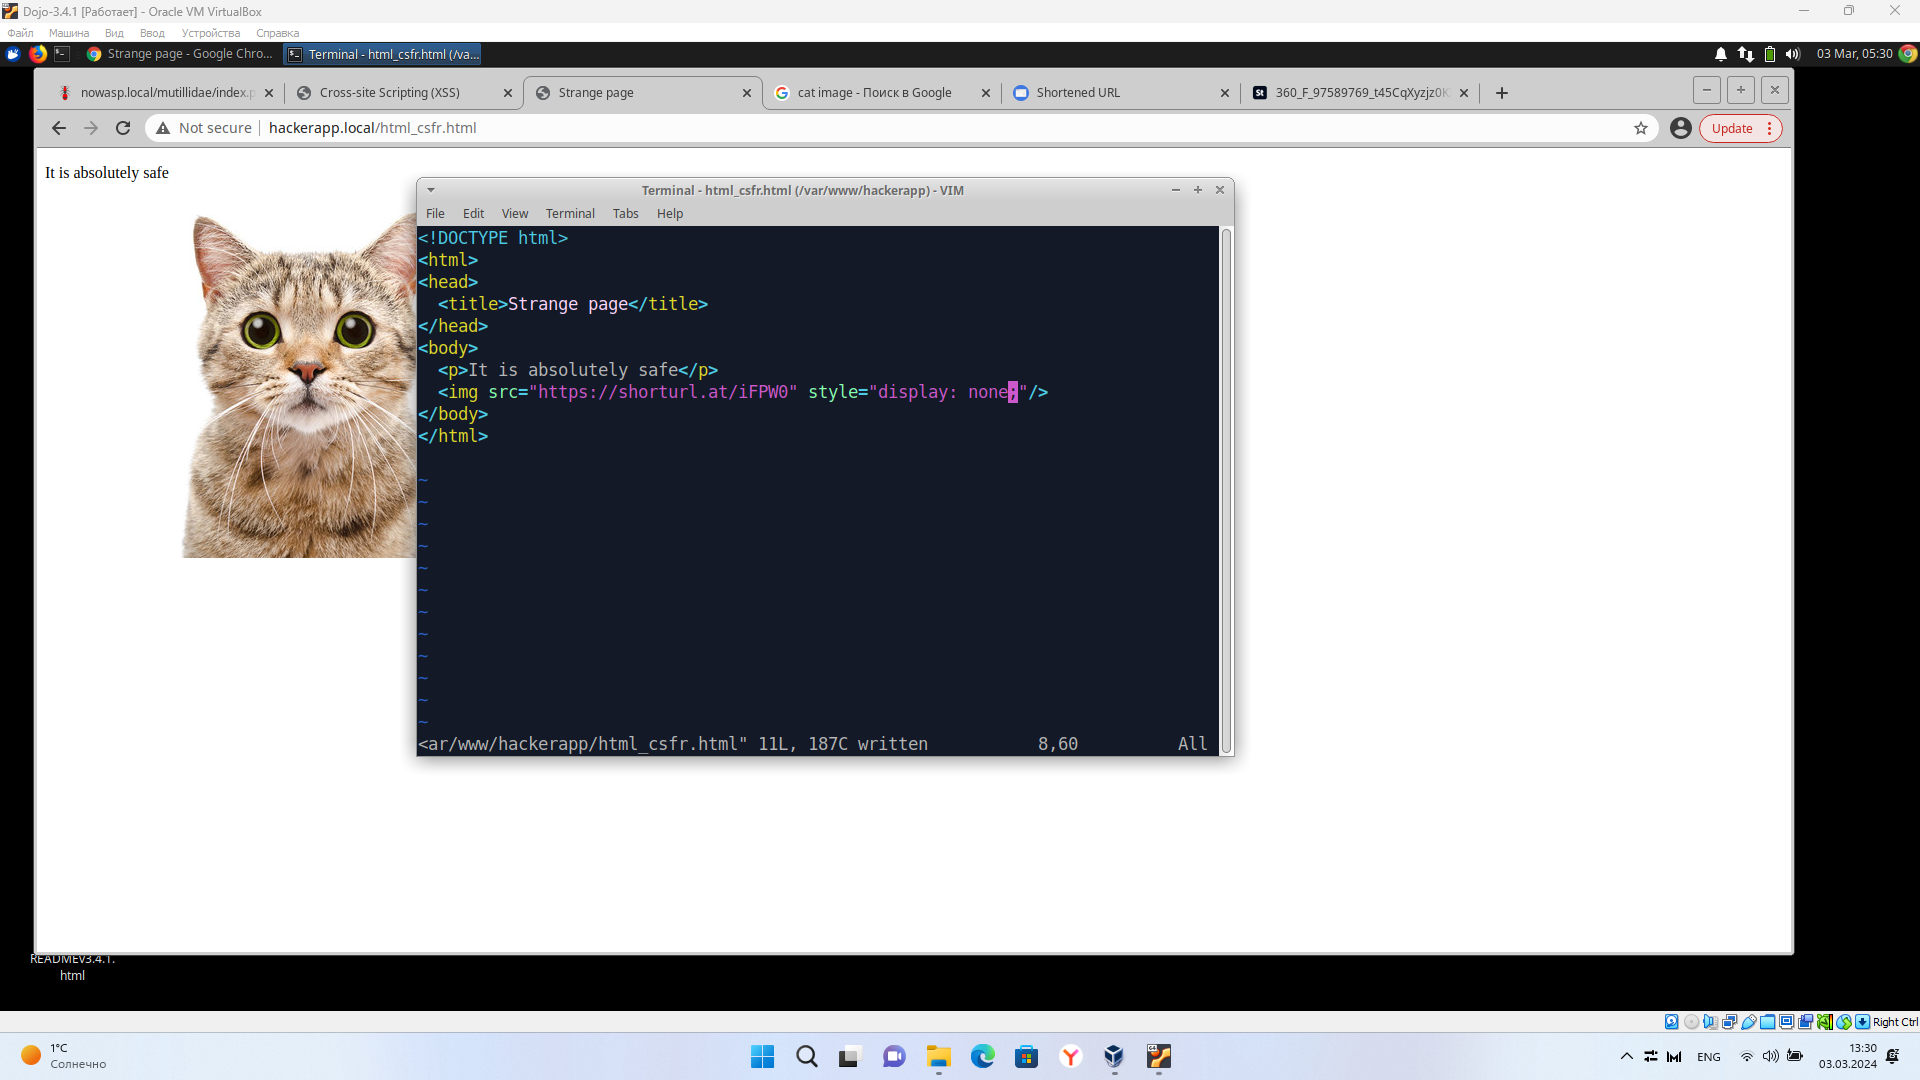
\includegraphics[width=\textwidth]{Screenshot_39}
    \caption{Прописываем стиль, скрывающий изображение}
  \end{figure}

  \begin{figure}[H]
    \centering
    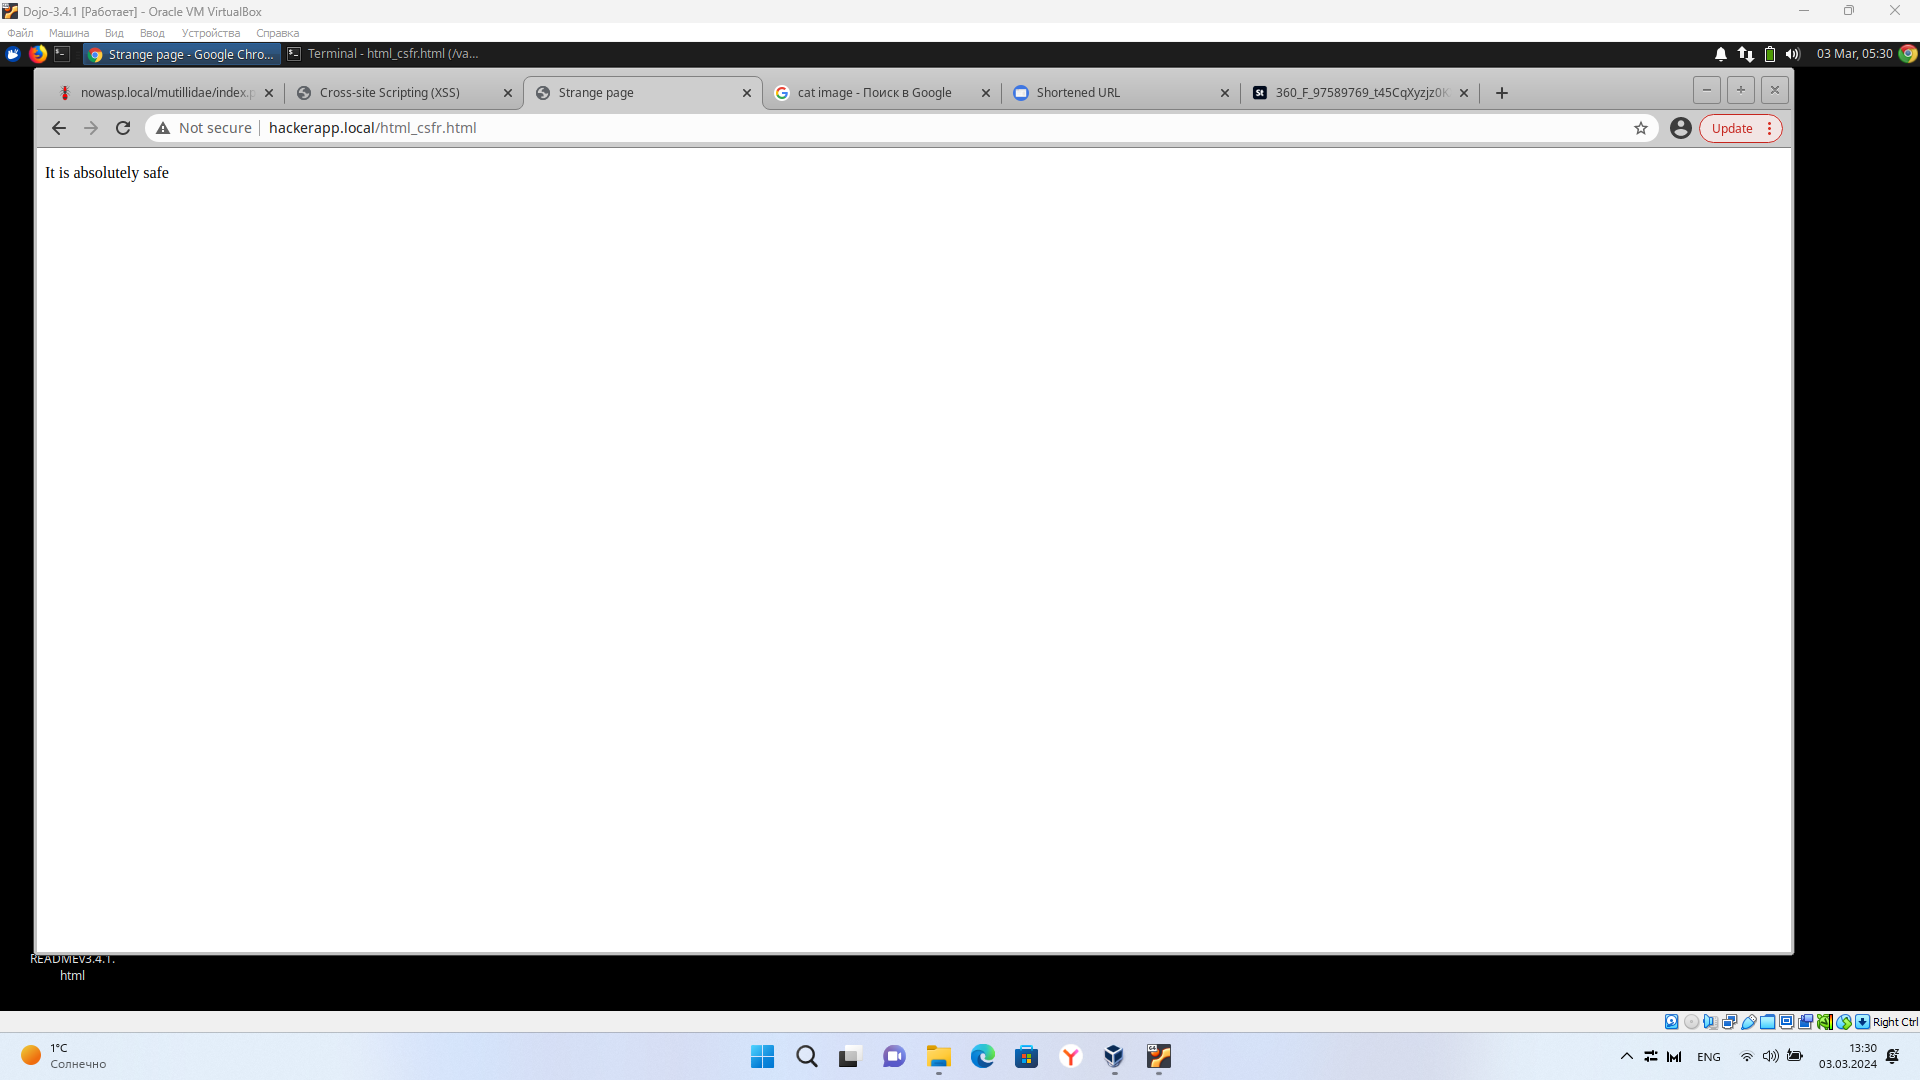
\includegraphics[width=\textwidth]{Screenshot_40}
    \caption{Картинка действительно пропала}
  \end{figure}

  \begin{figure}[H]
    \centering
    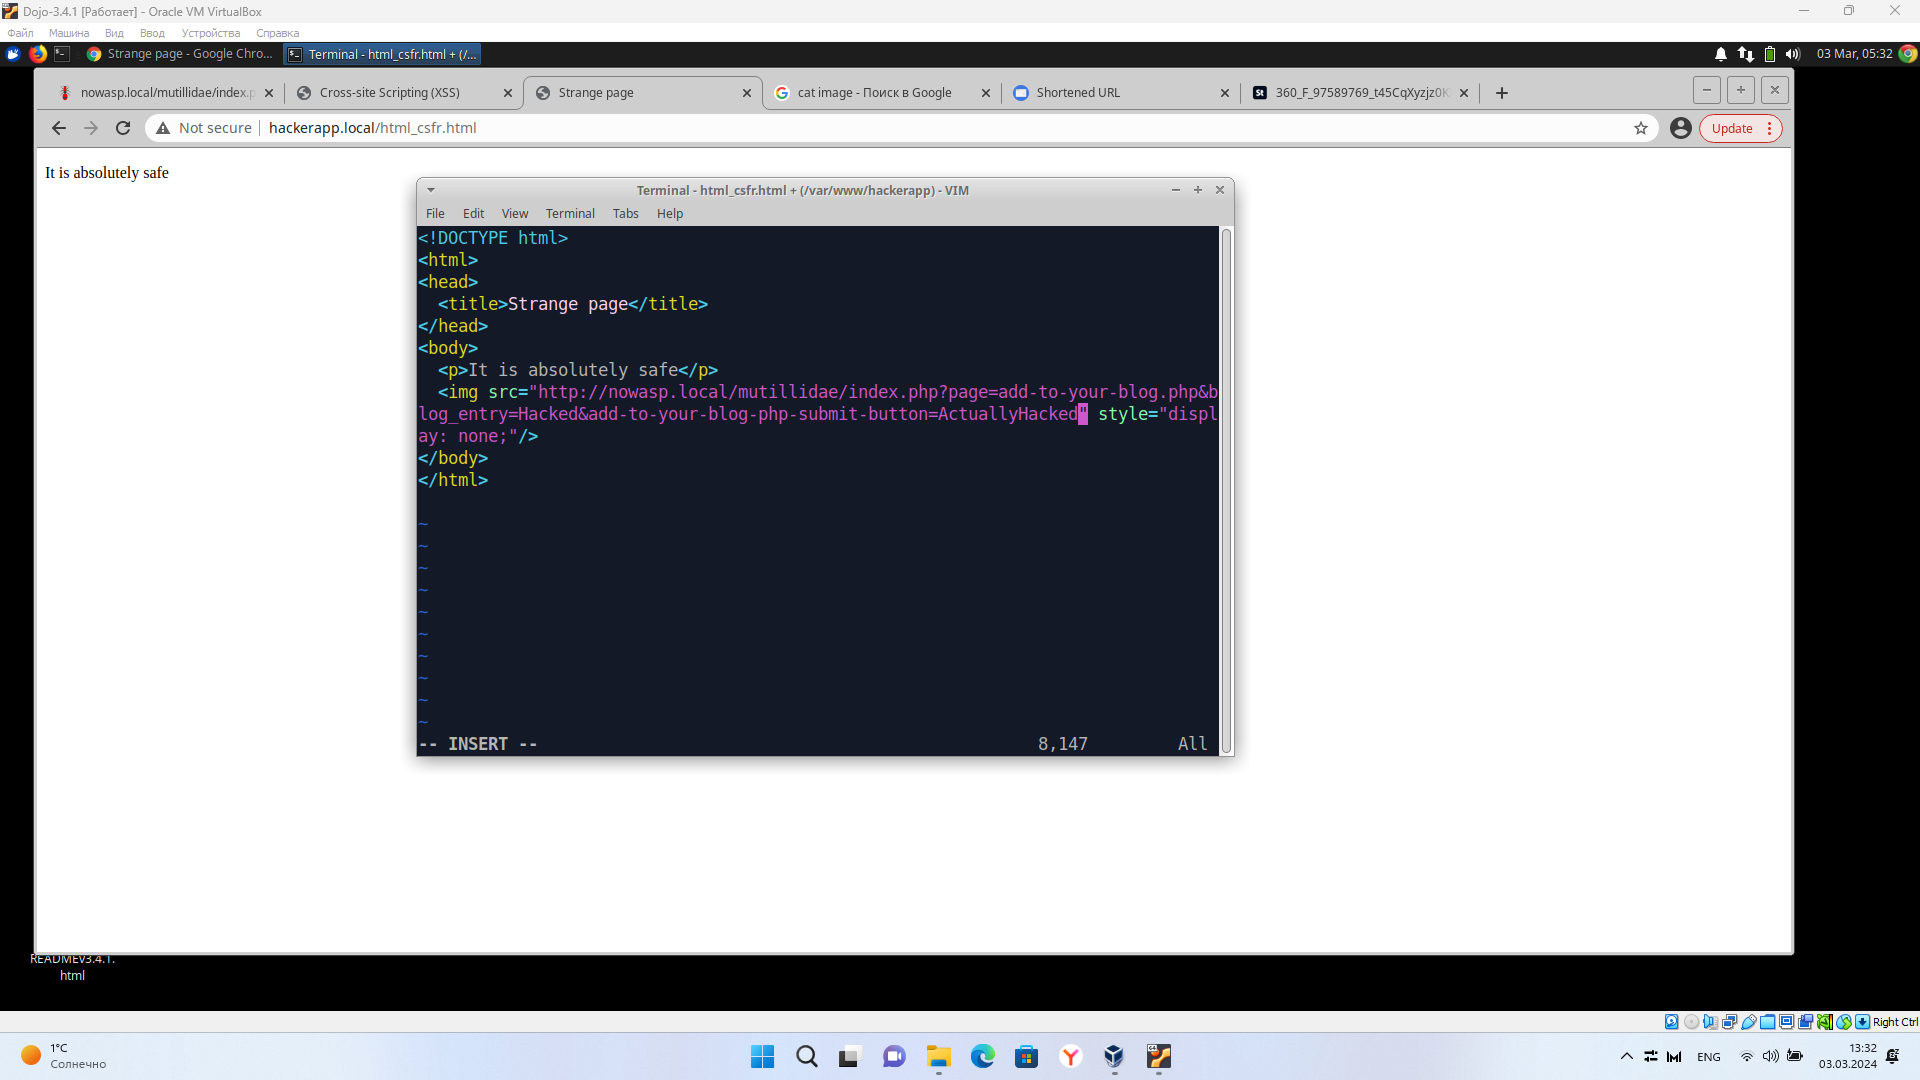
\includegraphics[width=\textwidth]{Screenshot_41}
    \caption{Подменяем ссылку на картинку на url для создания нового поста}
  \end{figure}

  \begin{figure}[H]
    \centering
    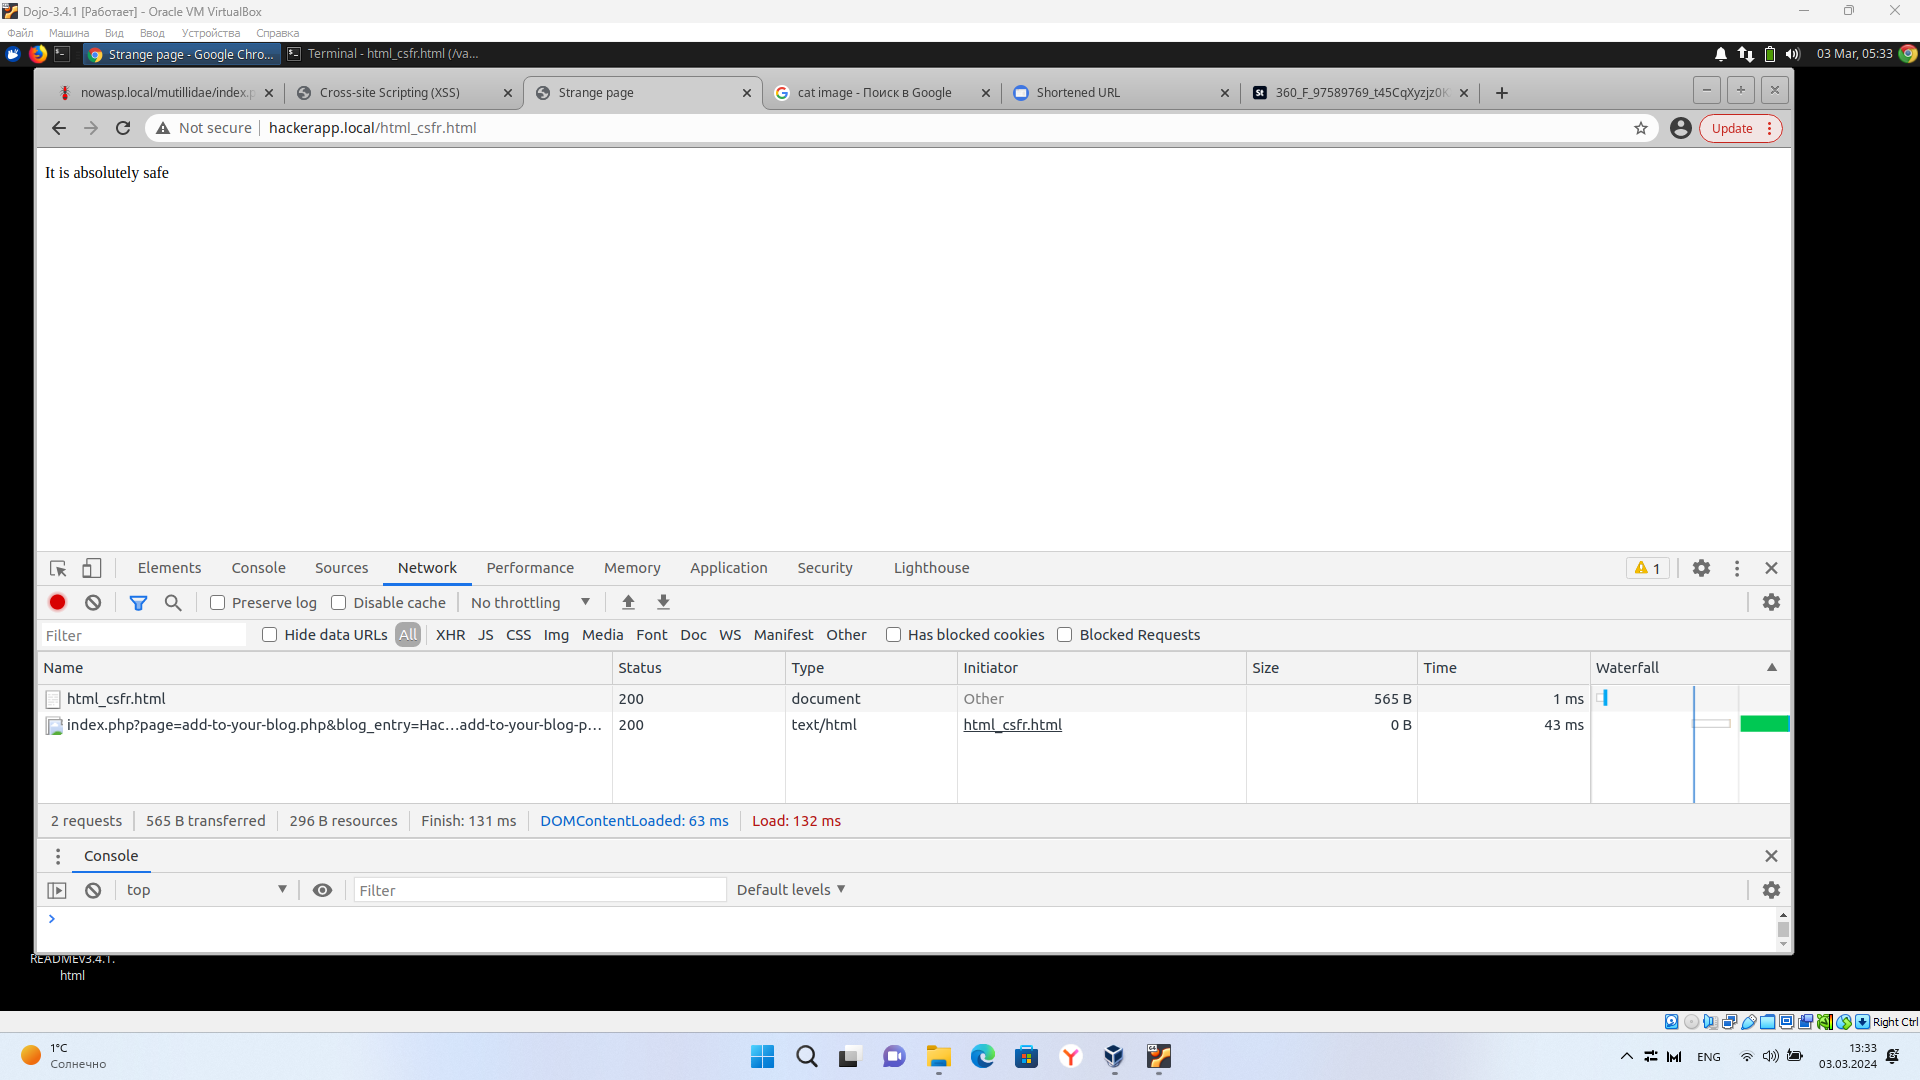
\includegraphics[width=\textwidth]{Screenshot_42}
    \caption{Пробуем загрузить страницу с опасным изображением}
  \end{figure}

  \begin{figure}[H]
    \centering
    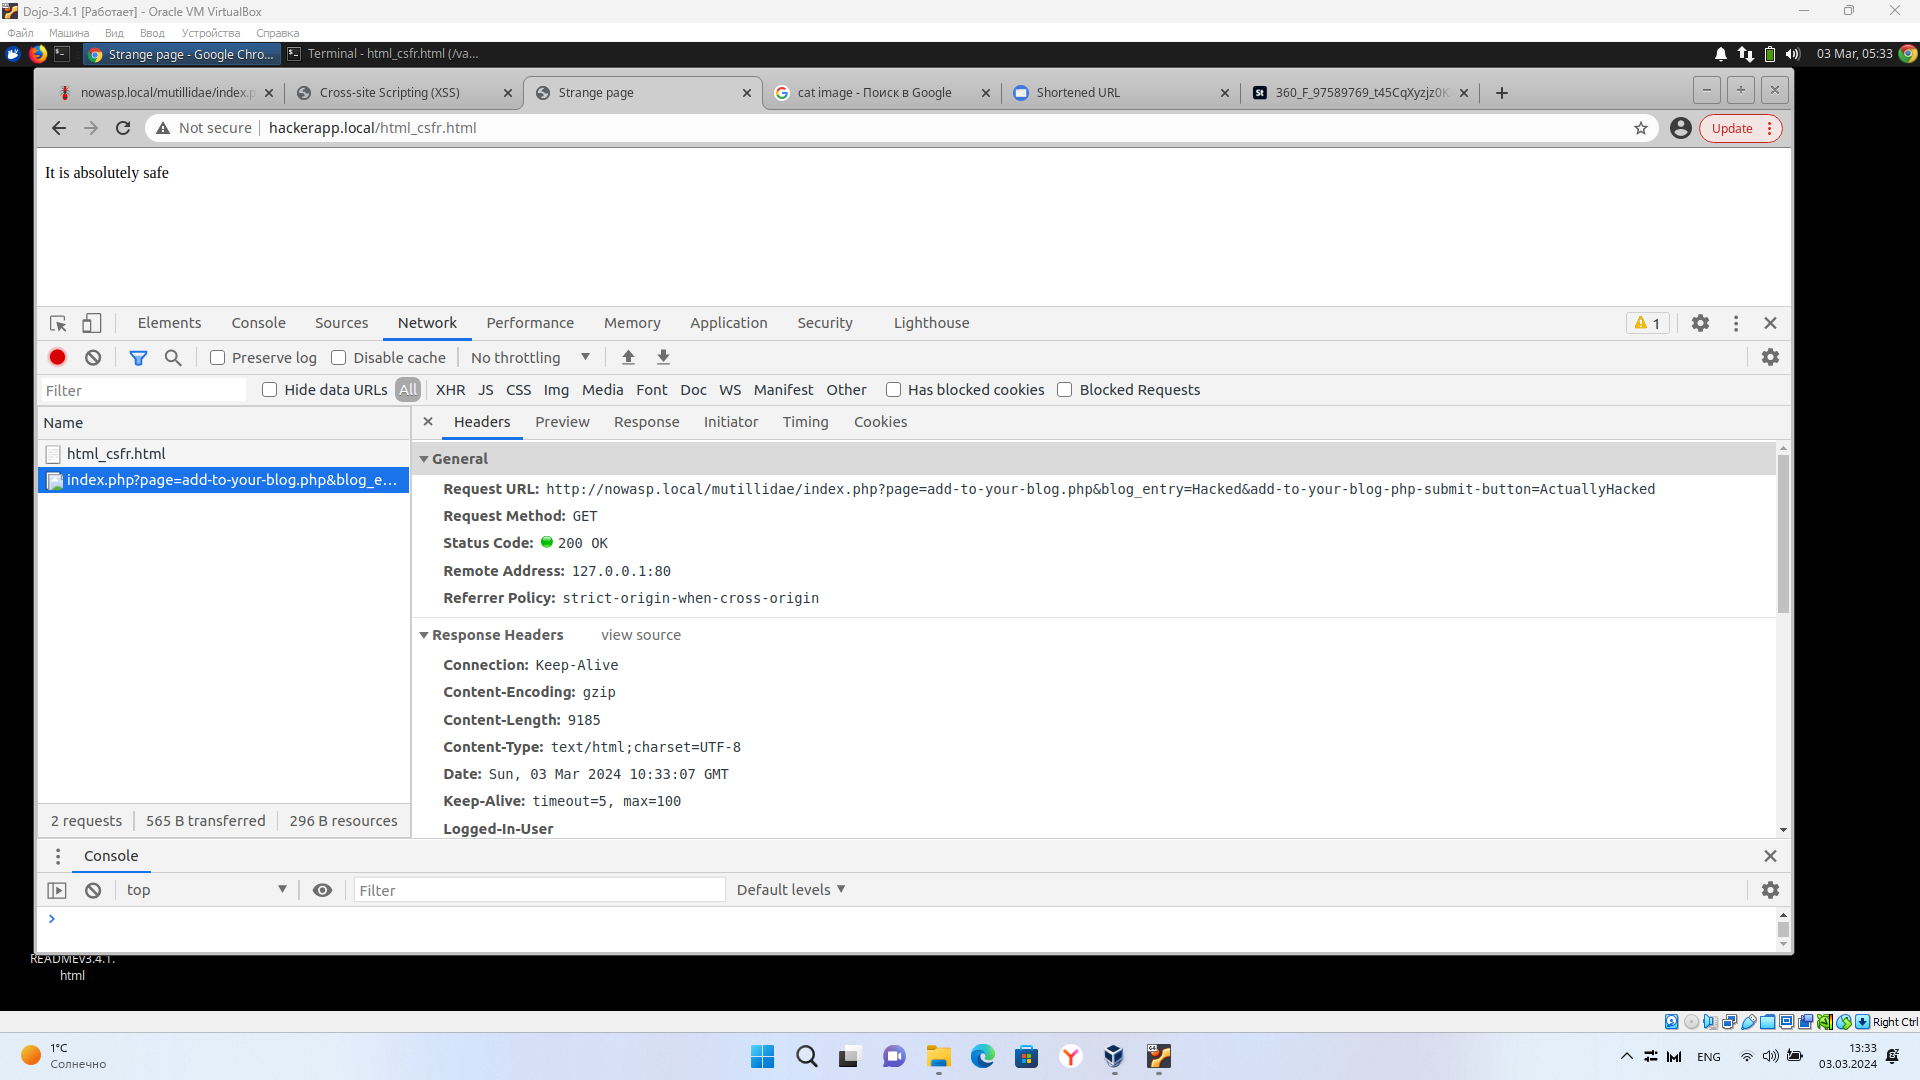
\includegraphics[width=\textwidth]{Screenshot_43}
    \caption{Видим, что выполнился запрос злоумышленника (меня)}
  \end{figure}

  Но этот запрос не сработал, так как это GET, а не POST запрос. Я заметил это только на этом моменте, поэтому пришлось
  переделывать на атку с использованием автоматически отправляемой html формы.

  \begin{figure}[H]
    \centering
    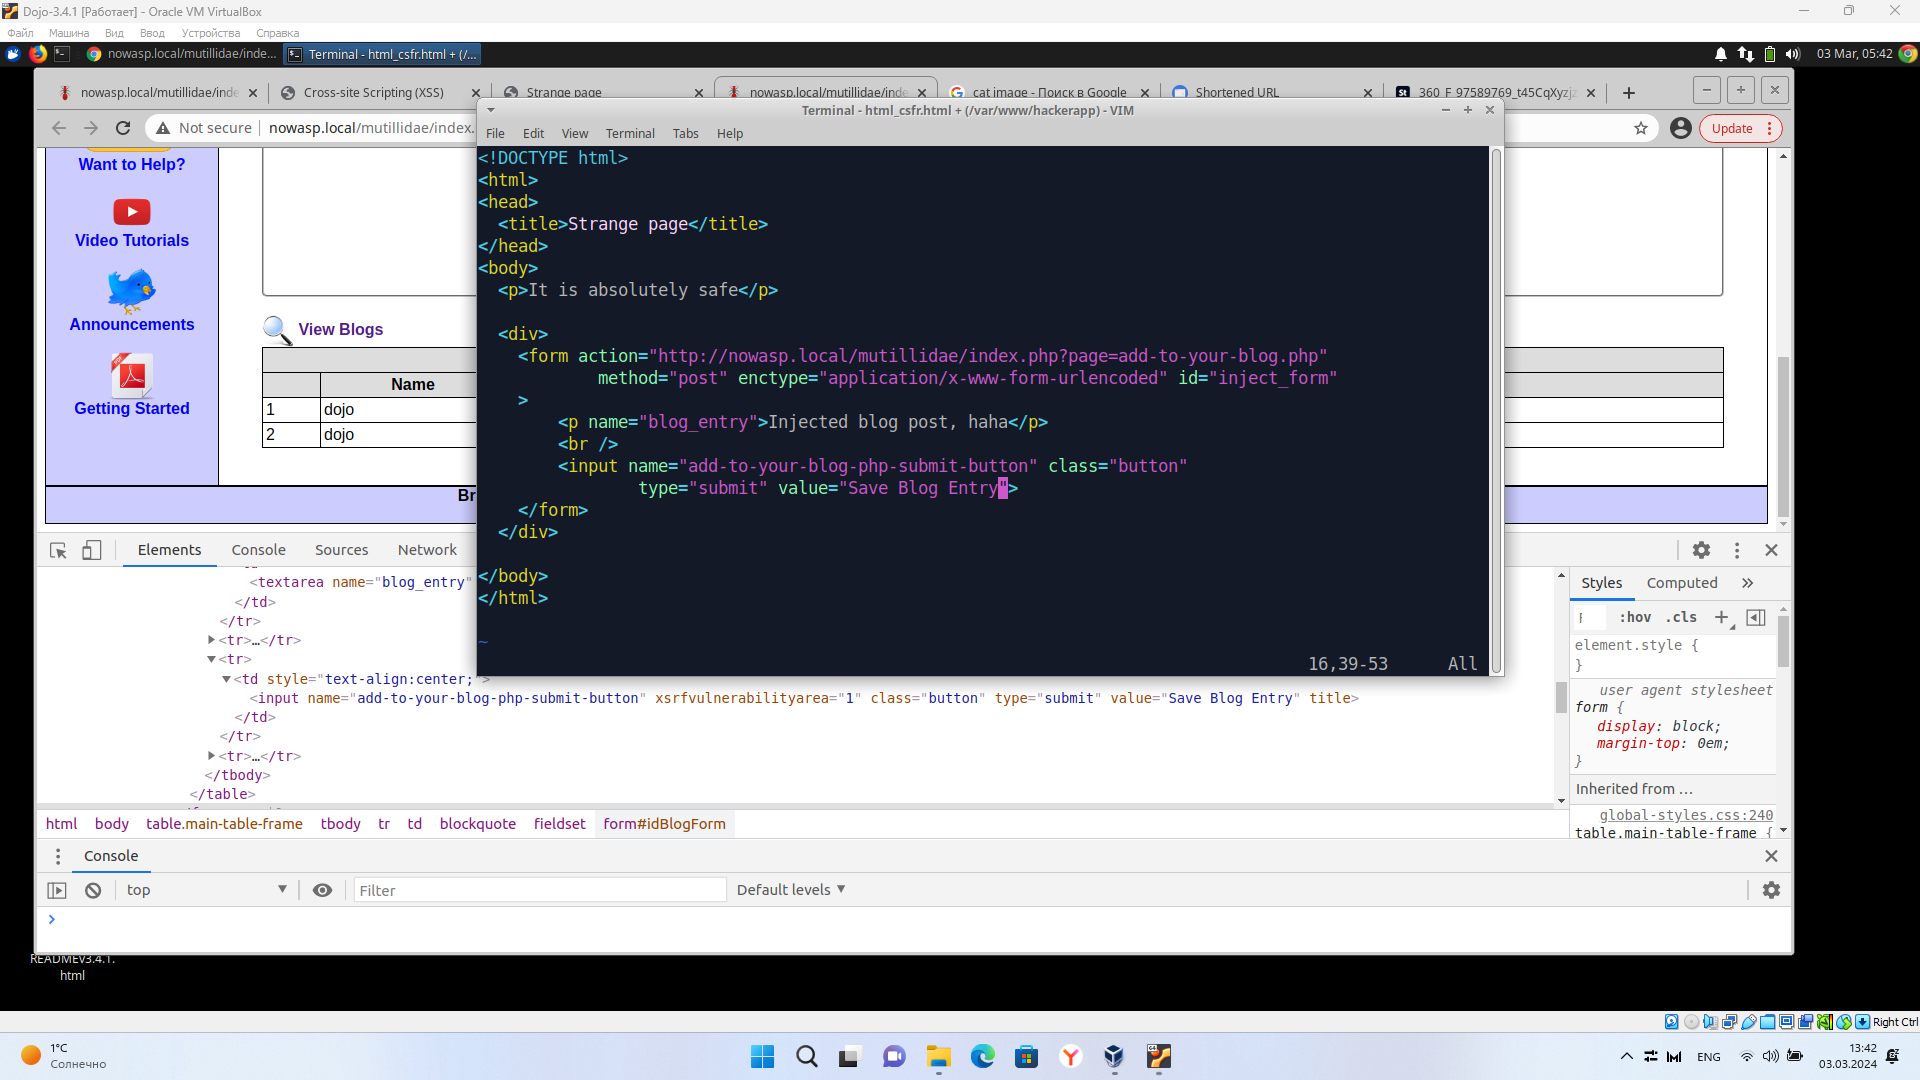
\includegraphics[width=\textwidth]{Screenshot_44}
    \caption{Добавляем форму для выполнения атаки}
  \end{figure}

  \begin{figure}[H]
    \centering
    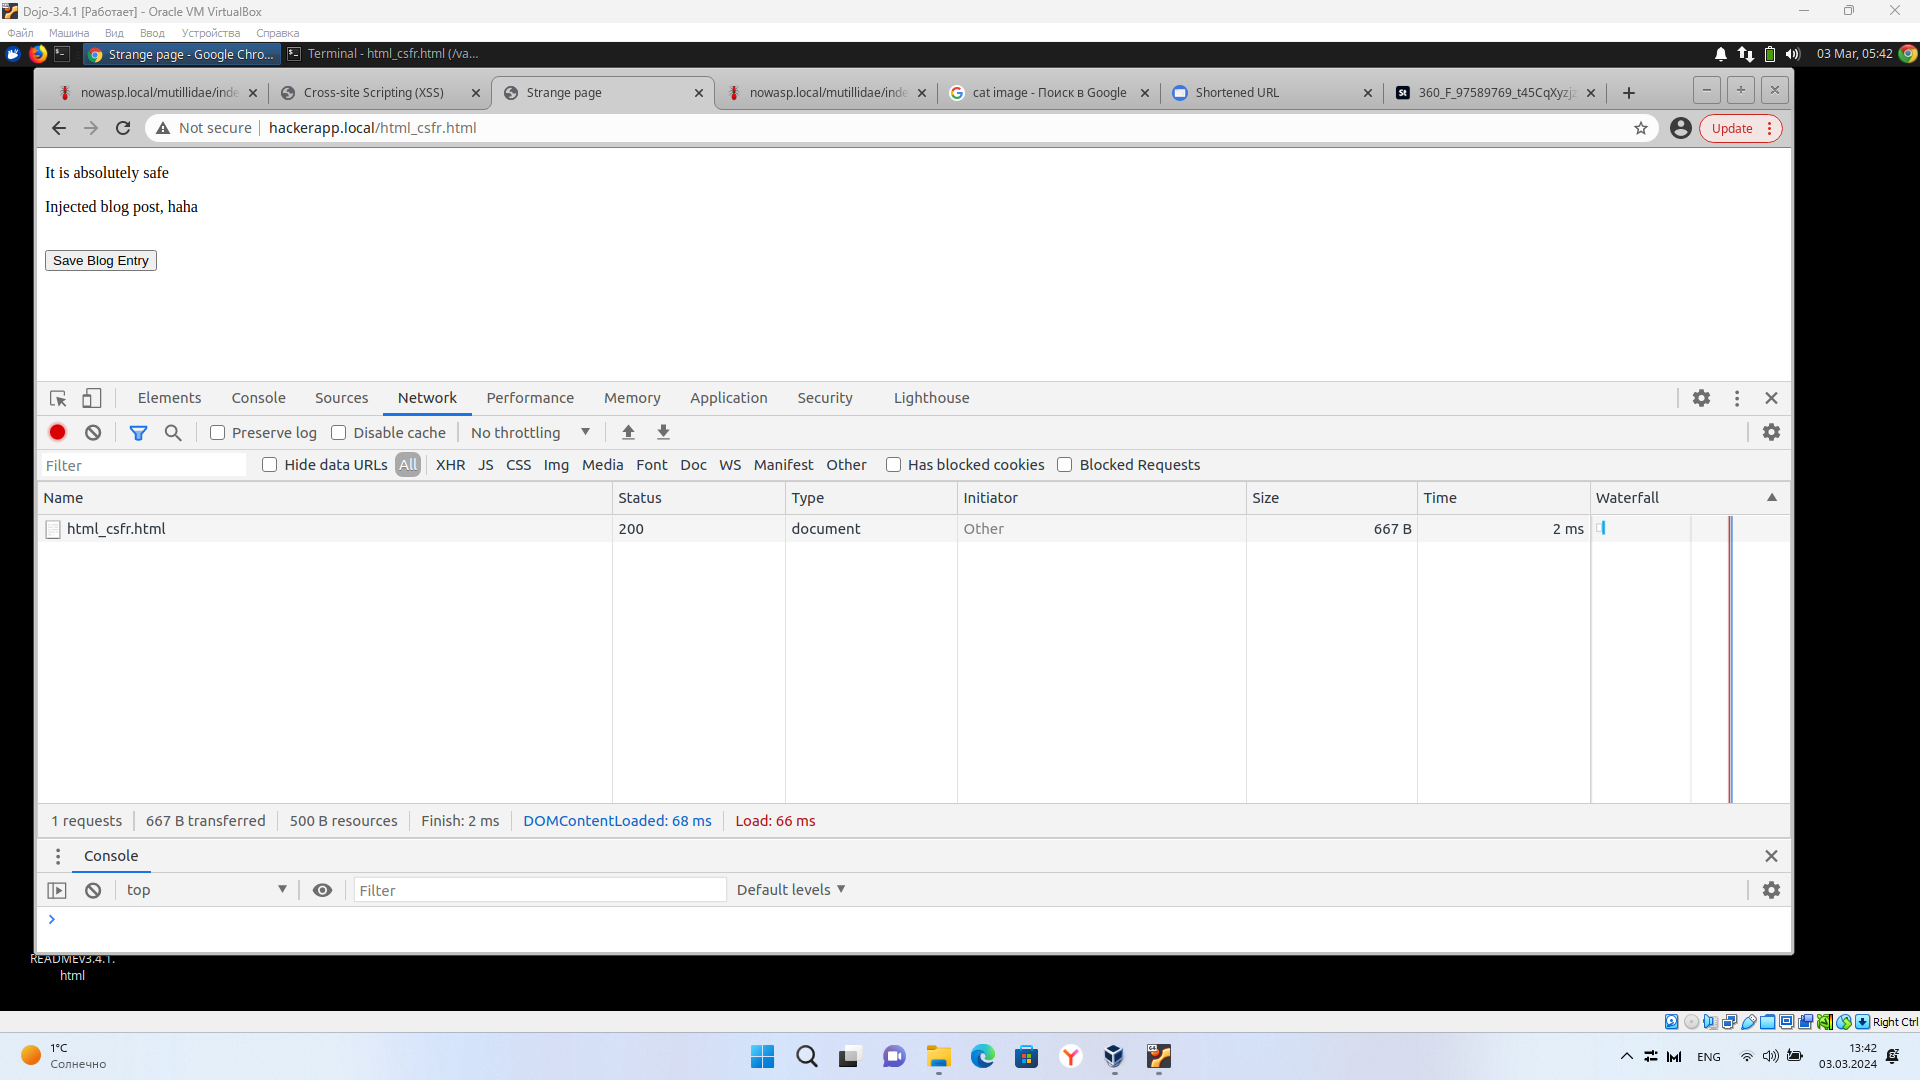
\includegraphics[width=\textwidth]{Screenshot_46}
    \caption{Пока эта форма требует ручной отправки, нажимаем кнопку}
  \end{figure}

  \begin{figure}[H]
    \centering
    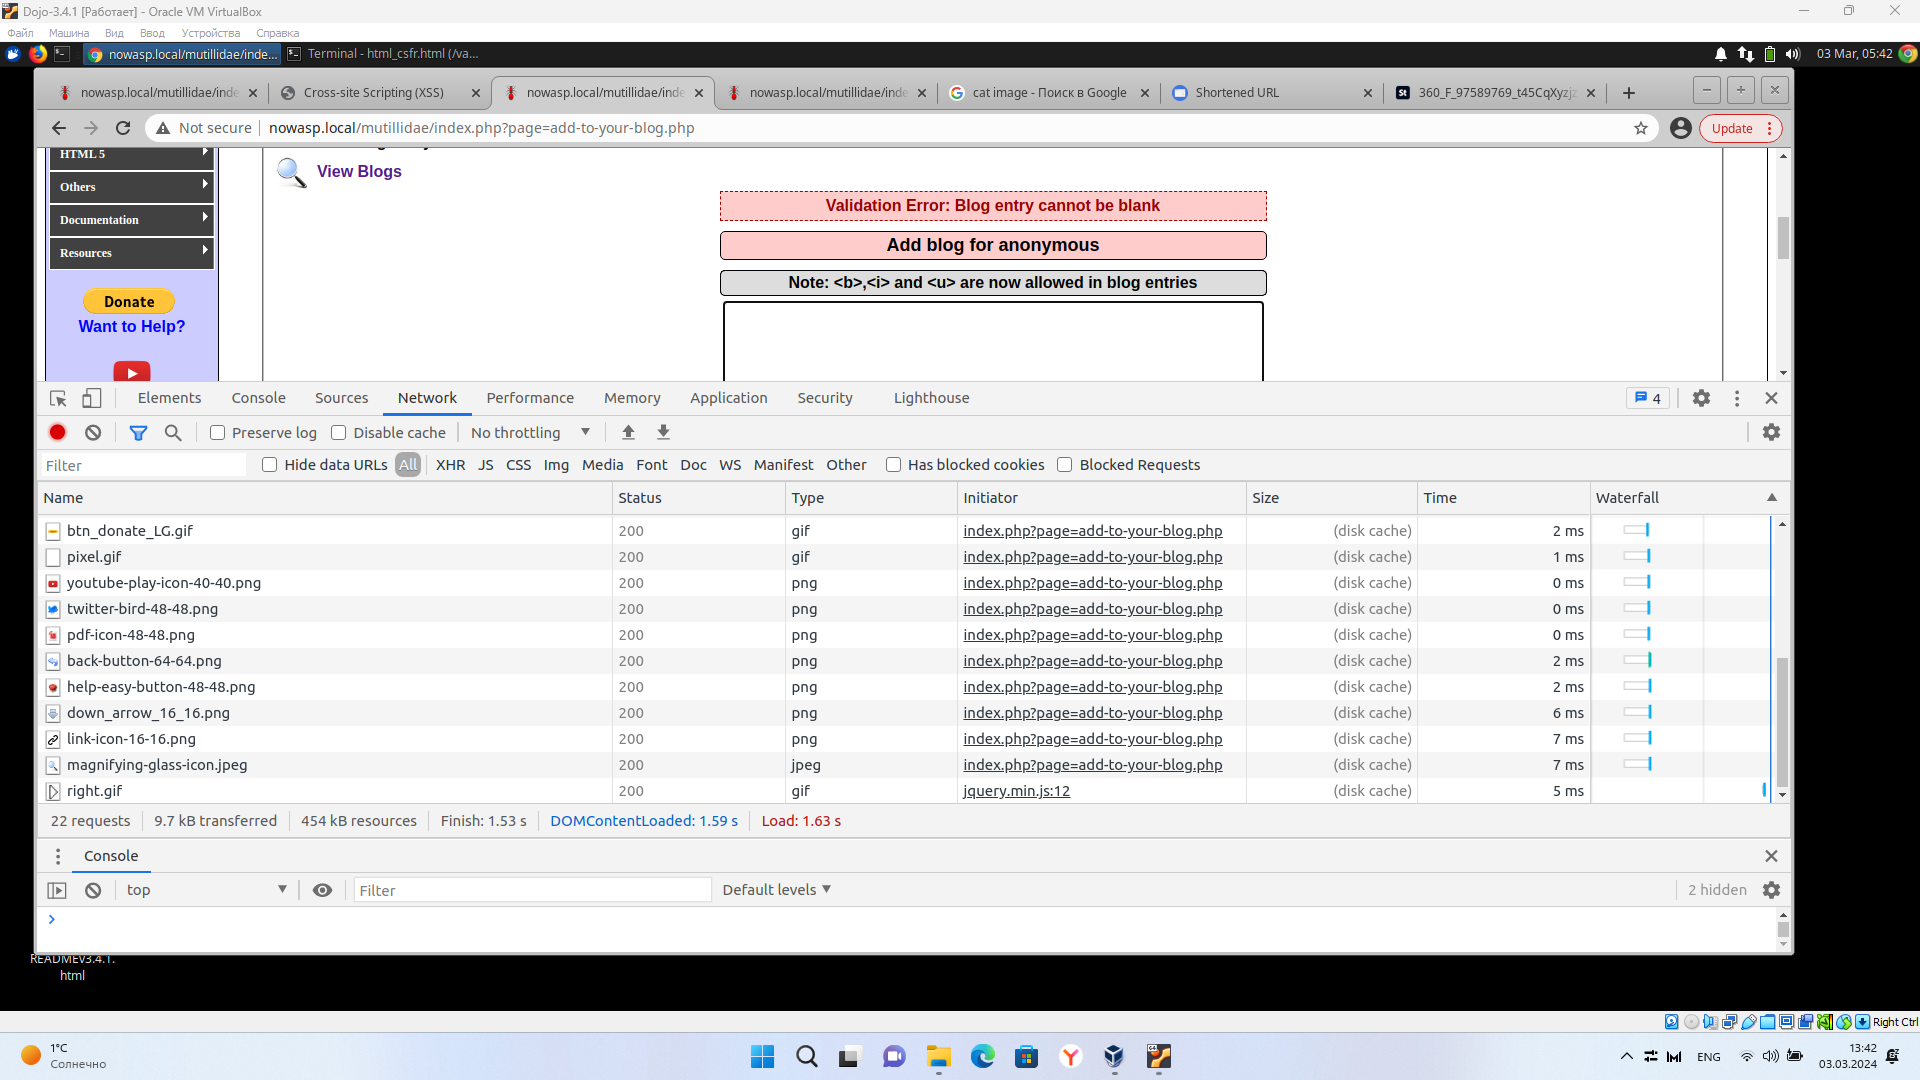
\includegraphics[width=\textwidth]{Screenshot_47}
    \caption{Ошибка, из-за неправильной разметки текст для нового поста не отправился в запросе}
  \end{figure}

  \begin{figure}[H]
    \centering
    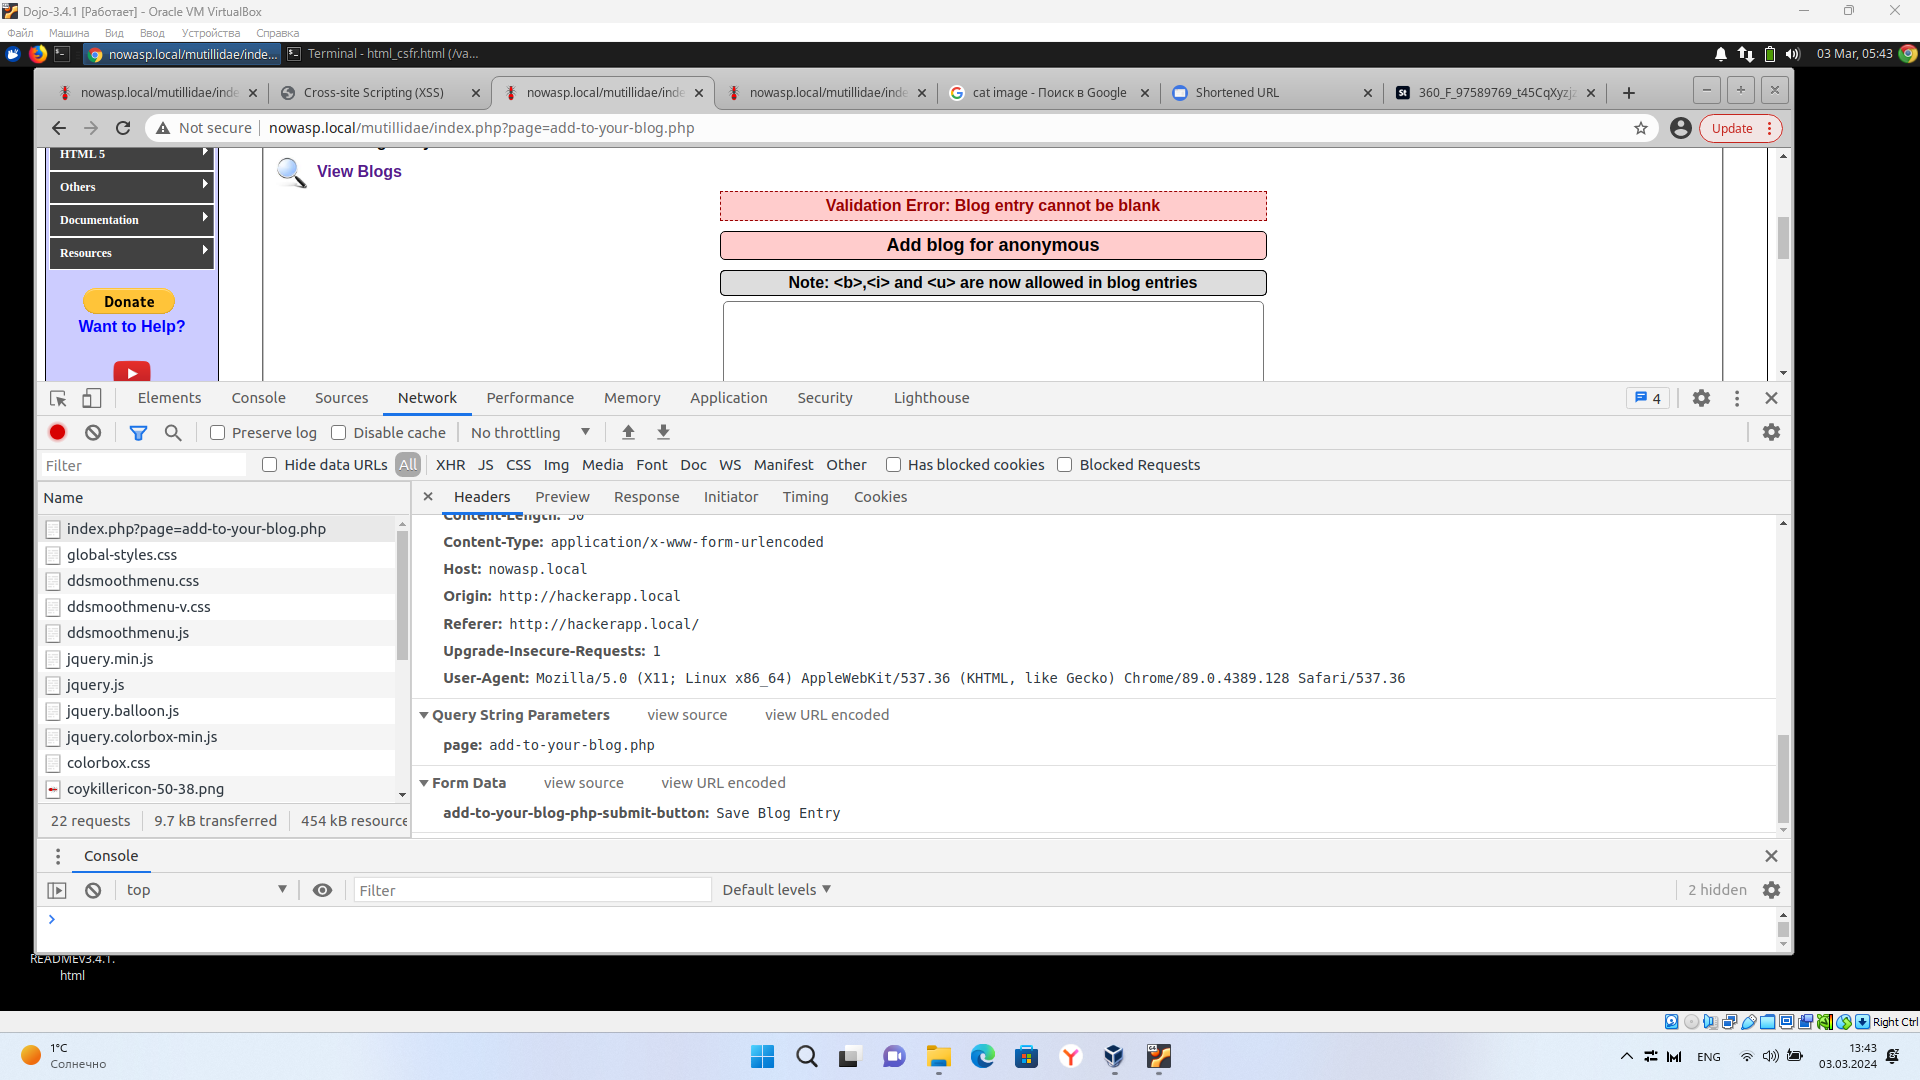
\includegraphics[width=\textwidth]{Screenshot_48}
    \caption{Поля blog entry действительно нет}
  \end{figure}

  \begin{figure}[H]
    \centering
    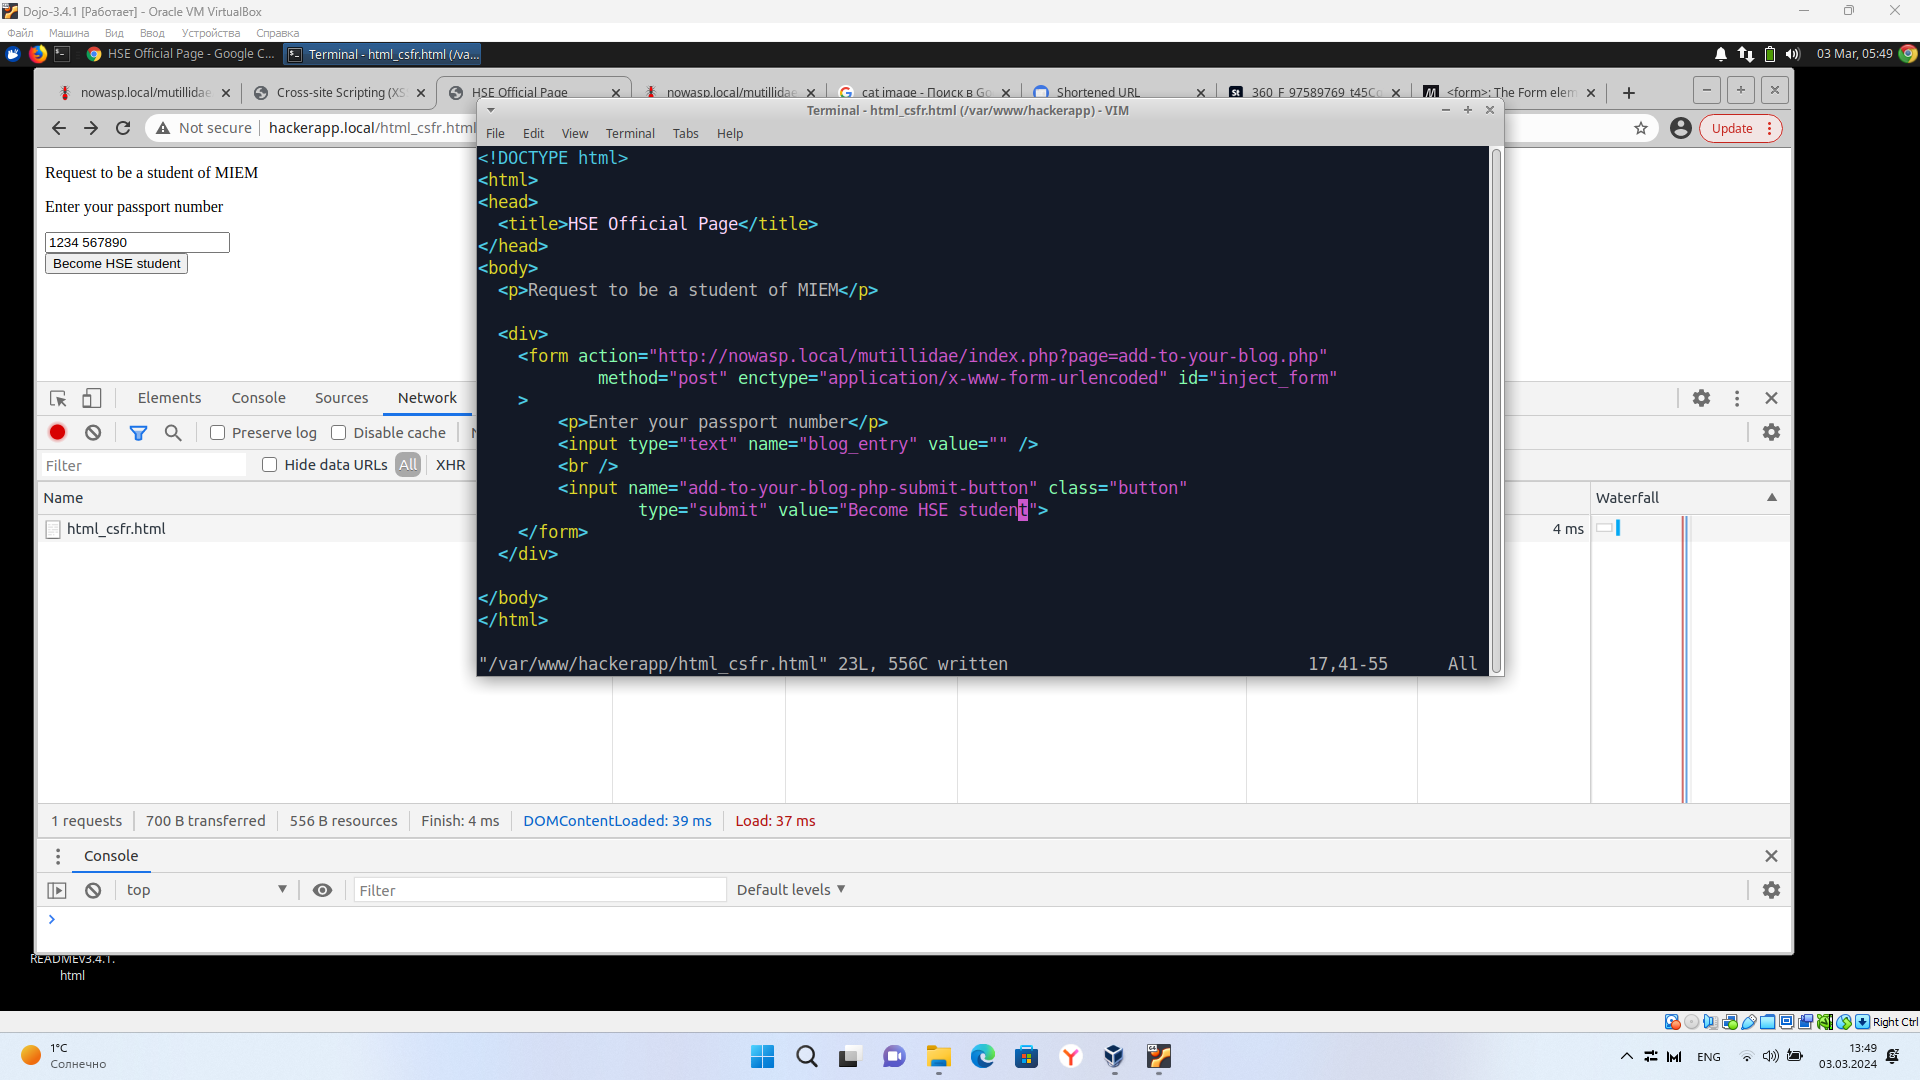
\includegraphics[width=\textwidth]{Screenshot_51}
    \caption{Делаем разметку для сайта злоумышленника}
  \end{figure}

  \begin{figure}[H]
    \centering
    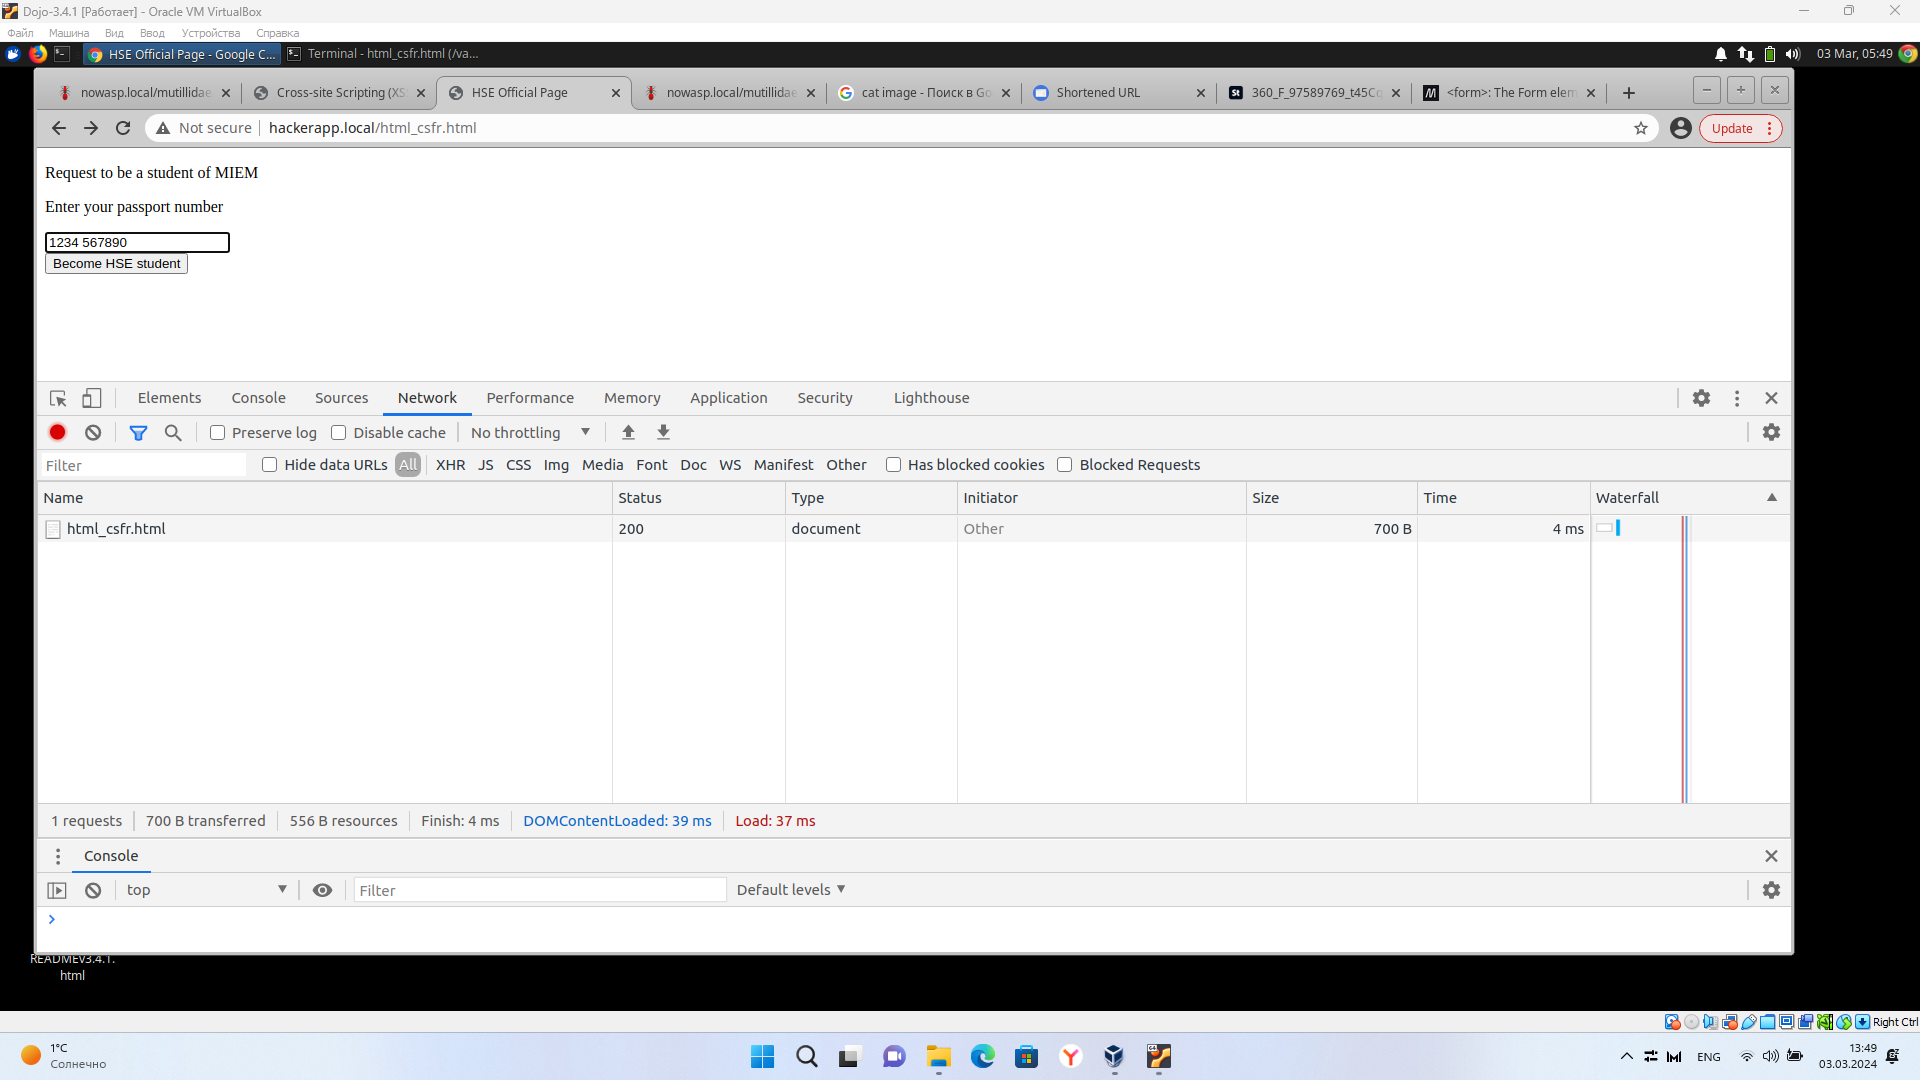
\includegraphics[width=\textwidth]{Screenshot_52}
    \caption{Жертва что-то вводит на сайте злоумышленника}
  \end{figure}

  \begin{figure}[H]
    \centering
    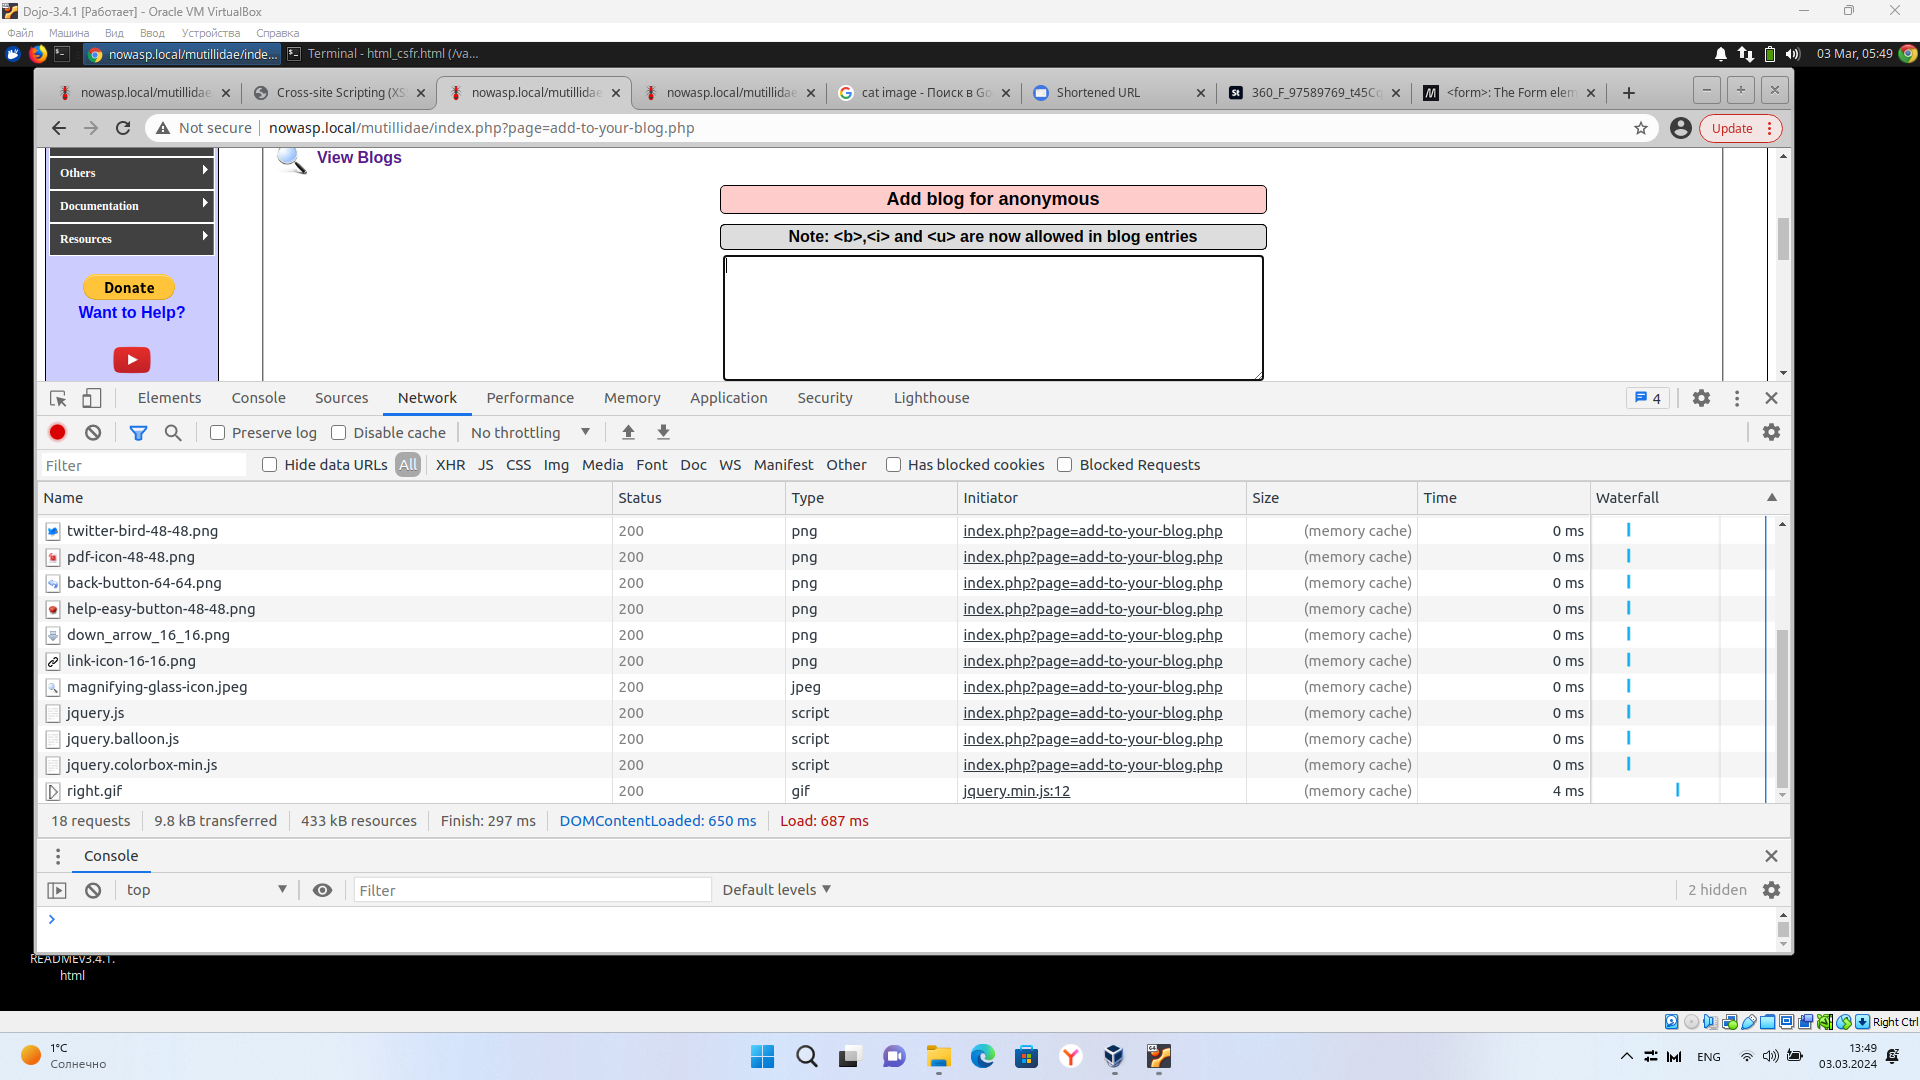
\includegraphics[width=\textwidth]{Screenshot_53}
    \caption{После нажатия на кнопку была создана новая запись для блога}
  \end{figure}

  \begin{figure}[H]
    \centering
    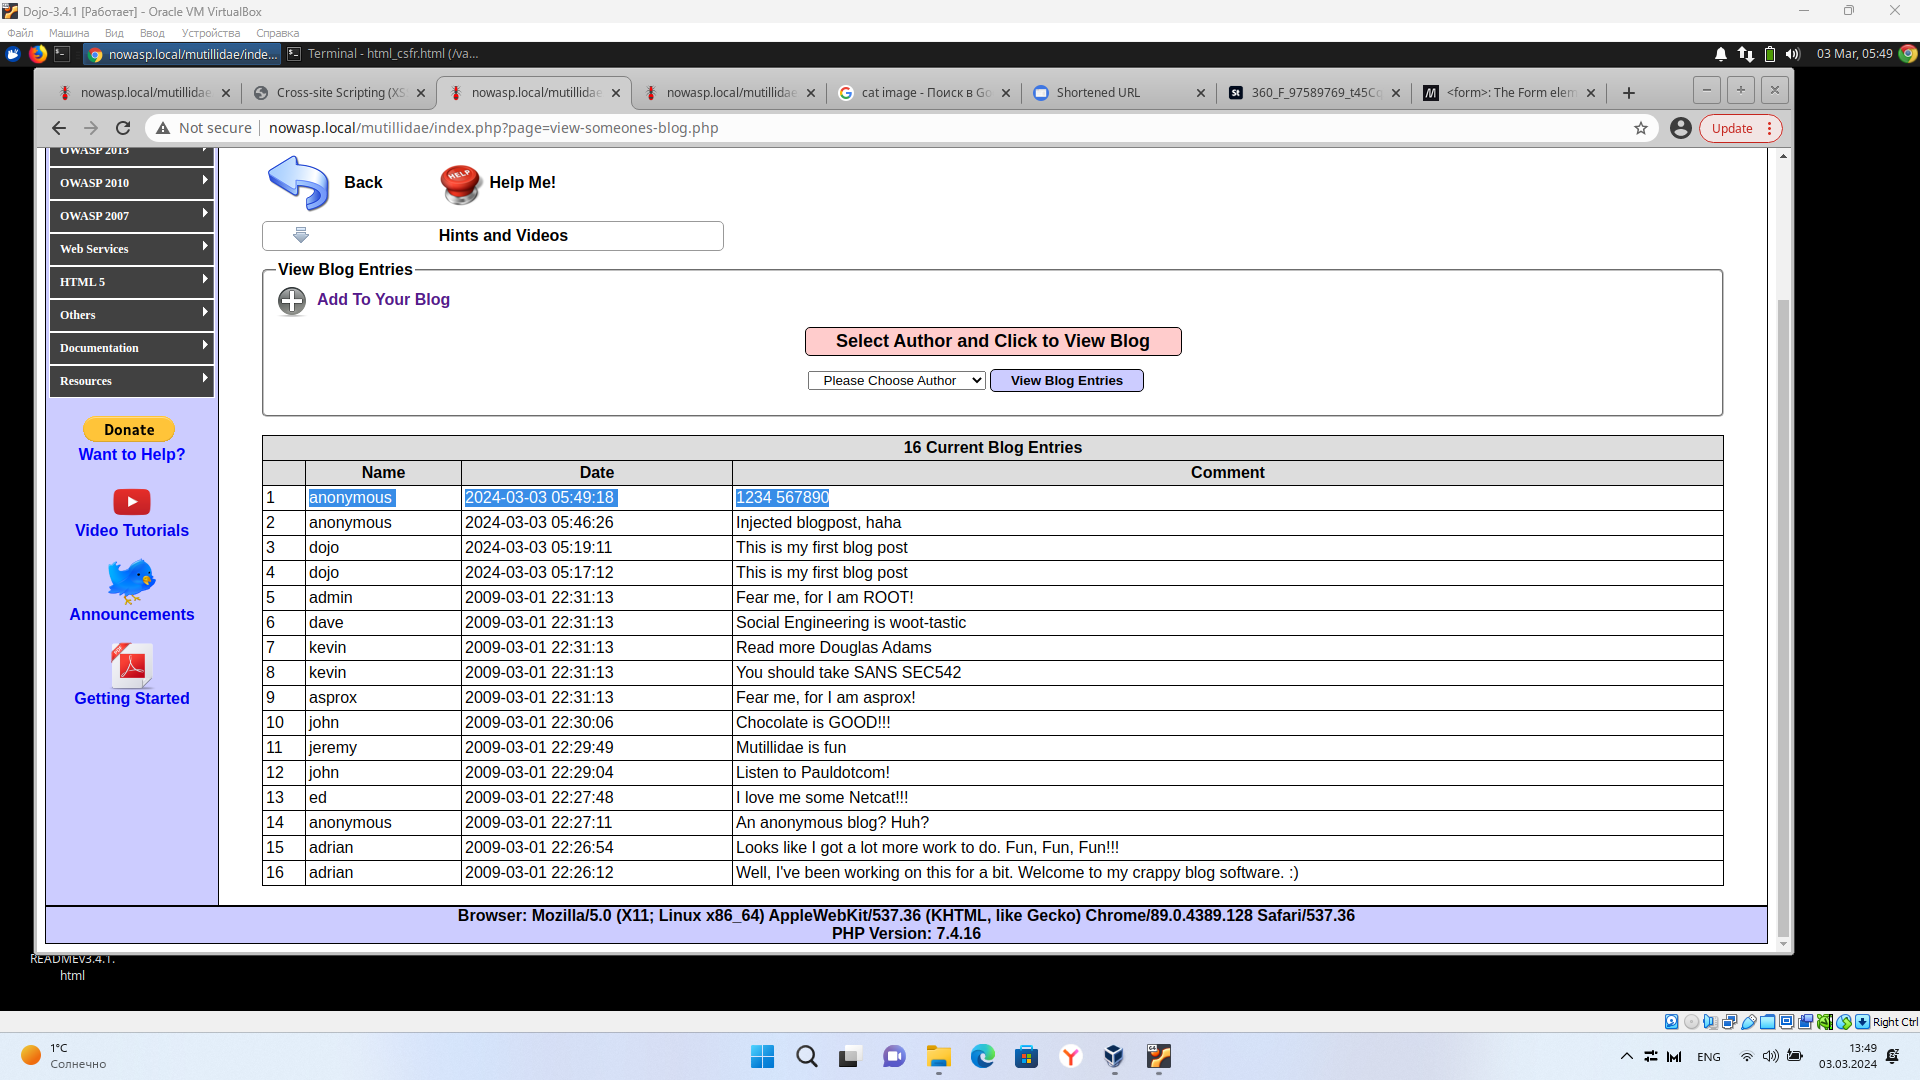
\includegraphics[width=\textwidth]{Screenshot_54}
    \caption{Видим ее в списке постов}
  \end{figure}

  \begin{figure}[H]
    \centering
    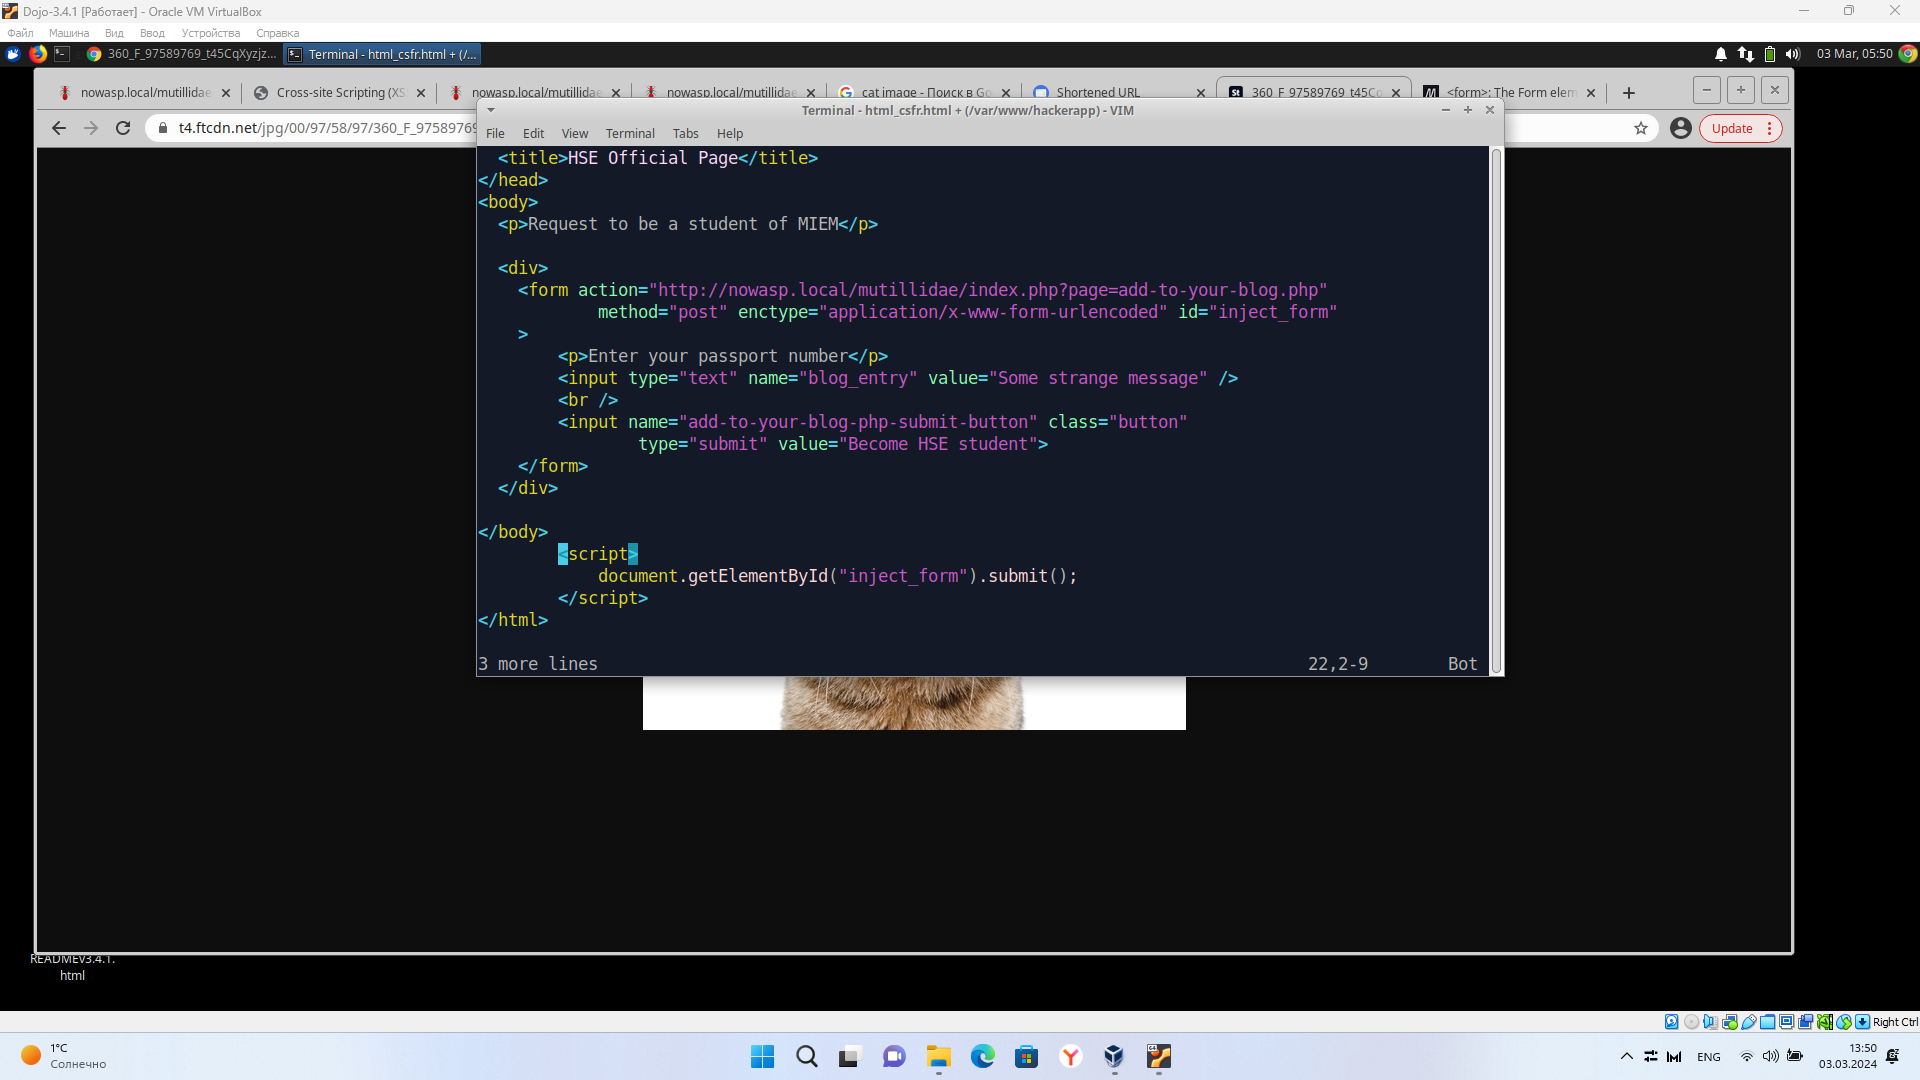
\includegraphics[width=\textwidth]{Screenshot_55}
    \caption{Добавим код для автоотправки формы}
  \end{figure}

  \begin{figure}[H]
    \centering
    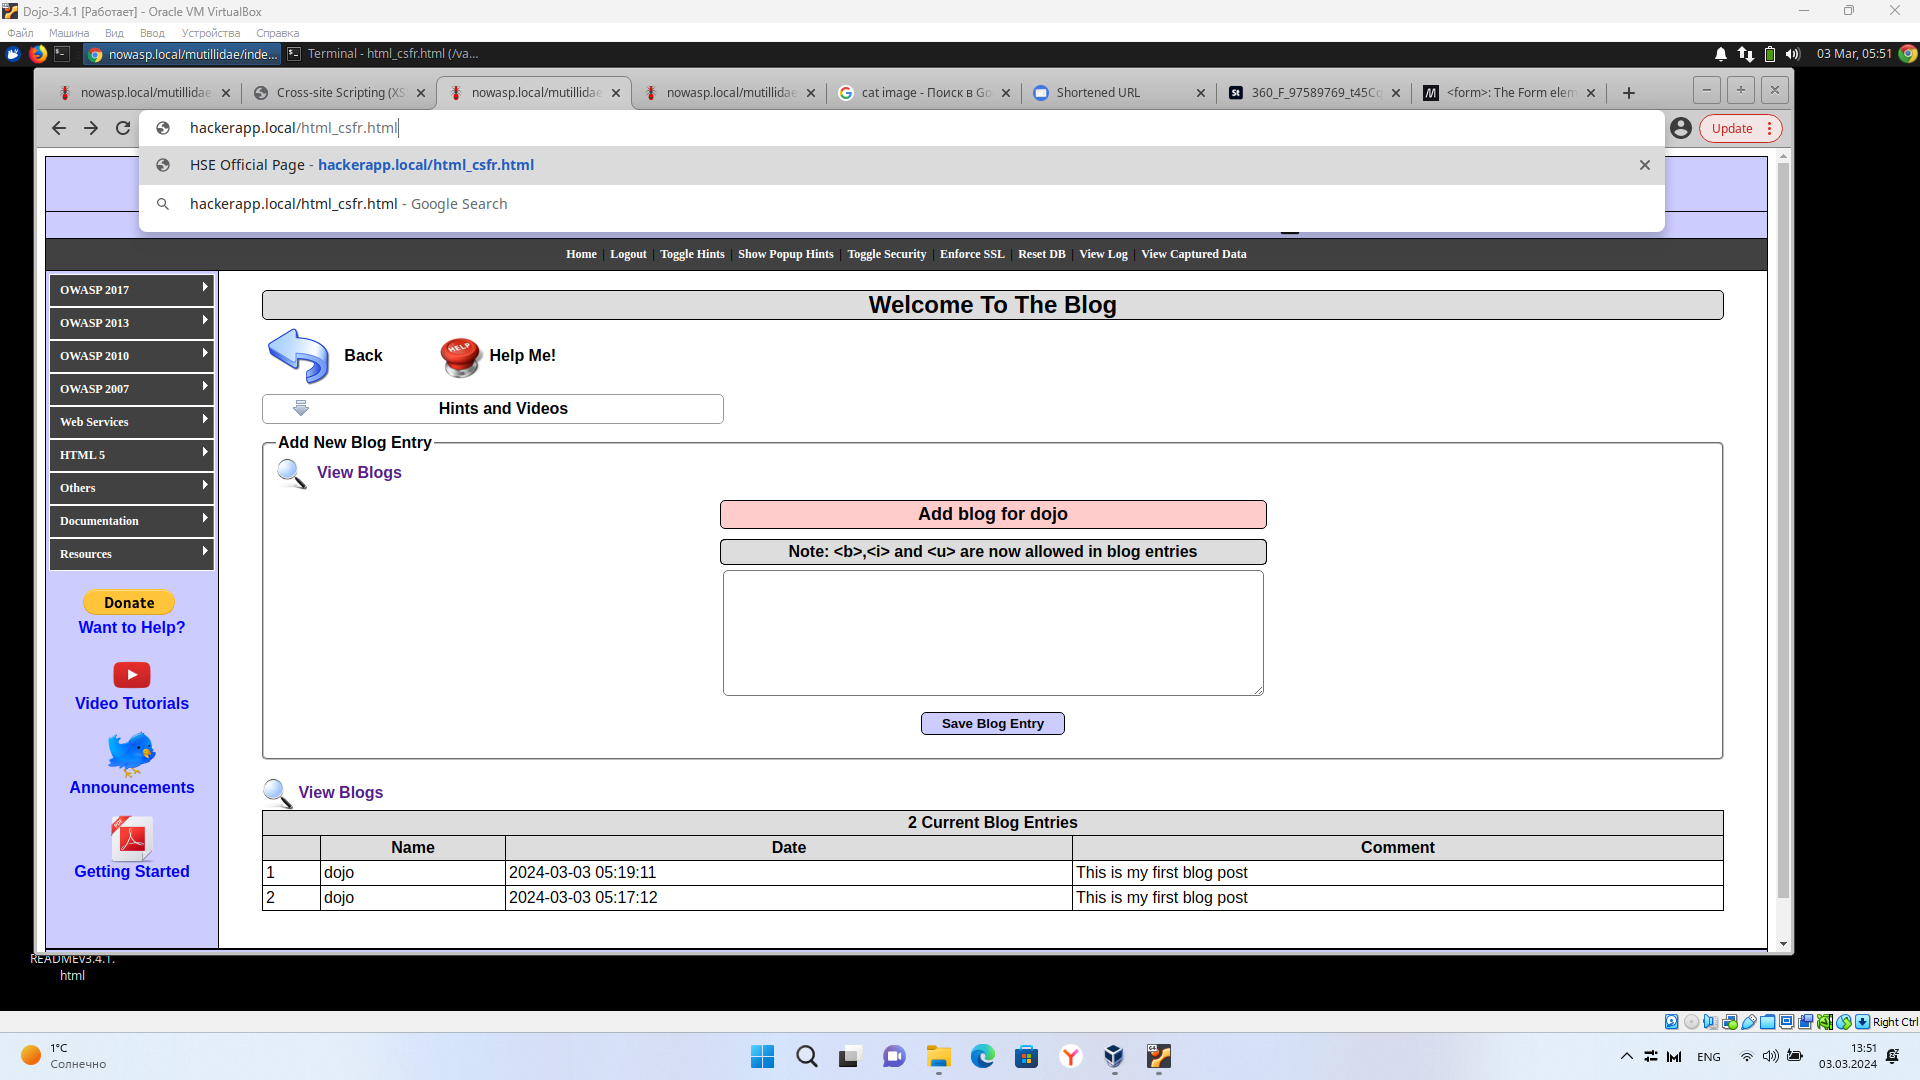
\includegraphics[width=\textwidth]{Screenshot_56}
    \caption{Переходим на сайт злоумышленника}
  \end{figure}

  \begin{figure}[H]
    \centering
    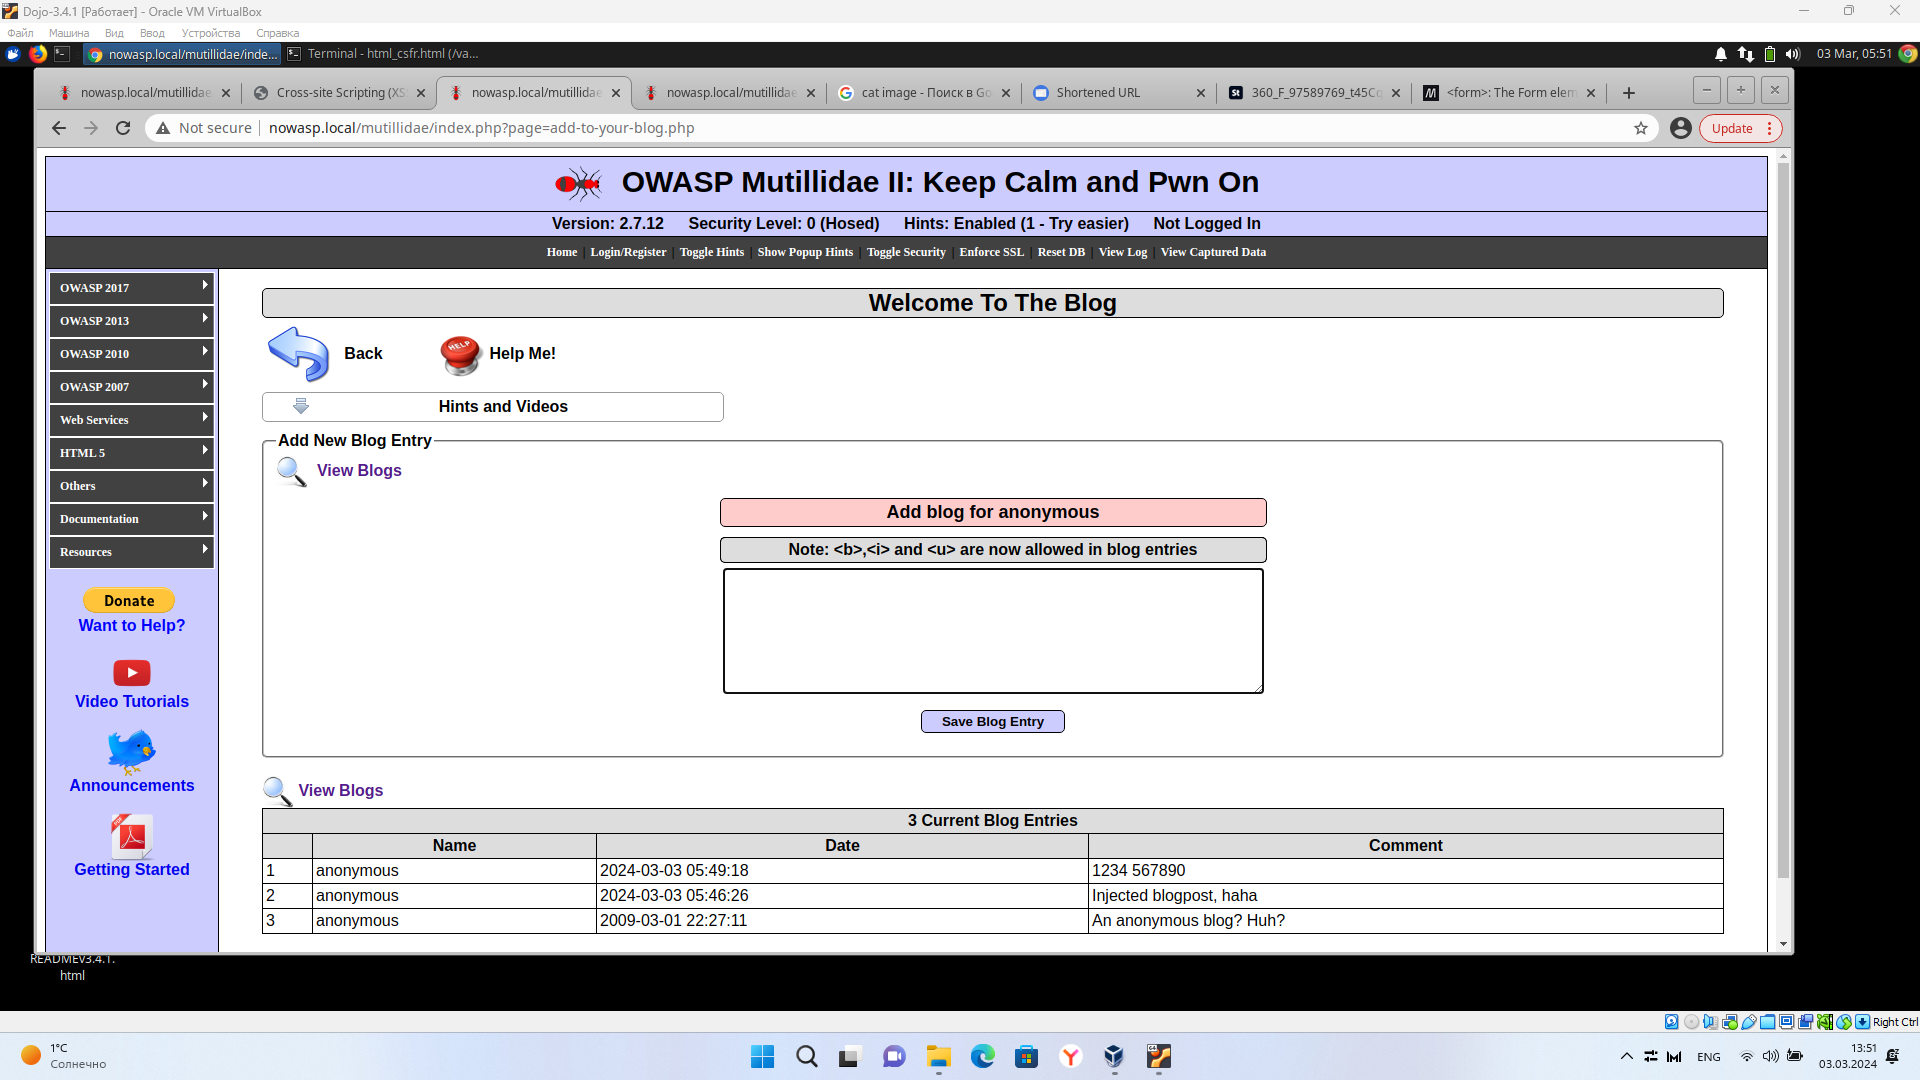
\includegraphics[width=\textwidth]{Screenshot_57}
    \caption{Создан новый пост - атака удалась}
  \end{figure}

  \begin{figure}[H]
    \centering
    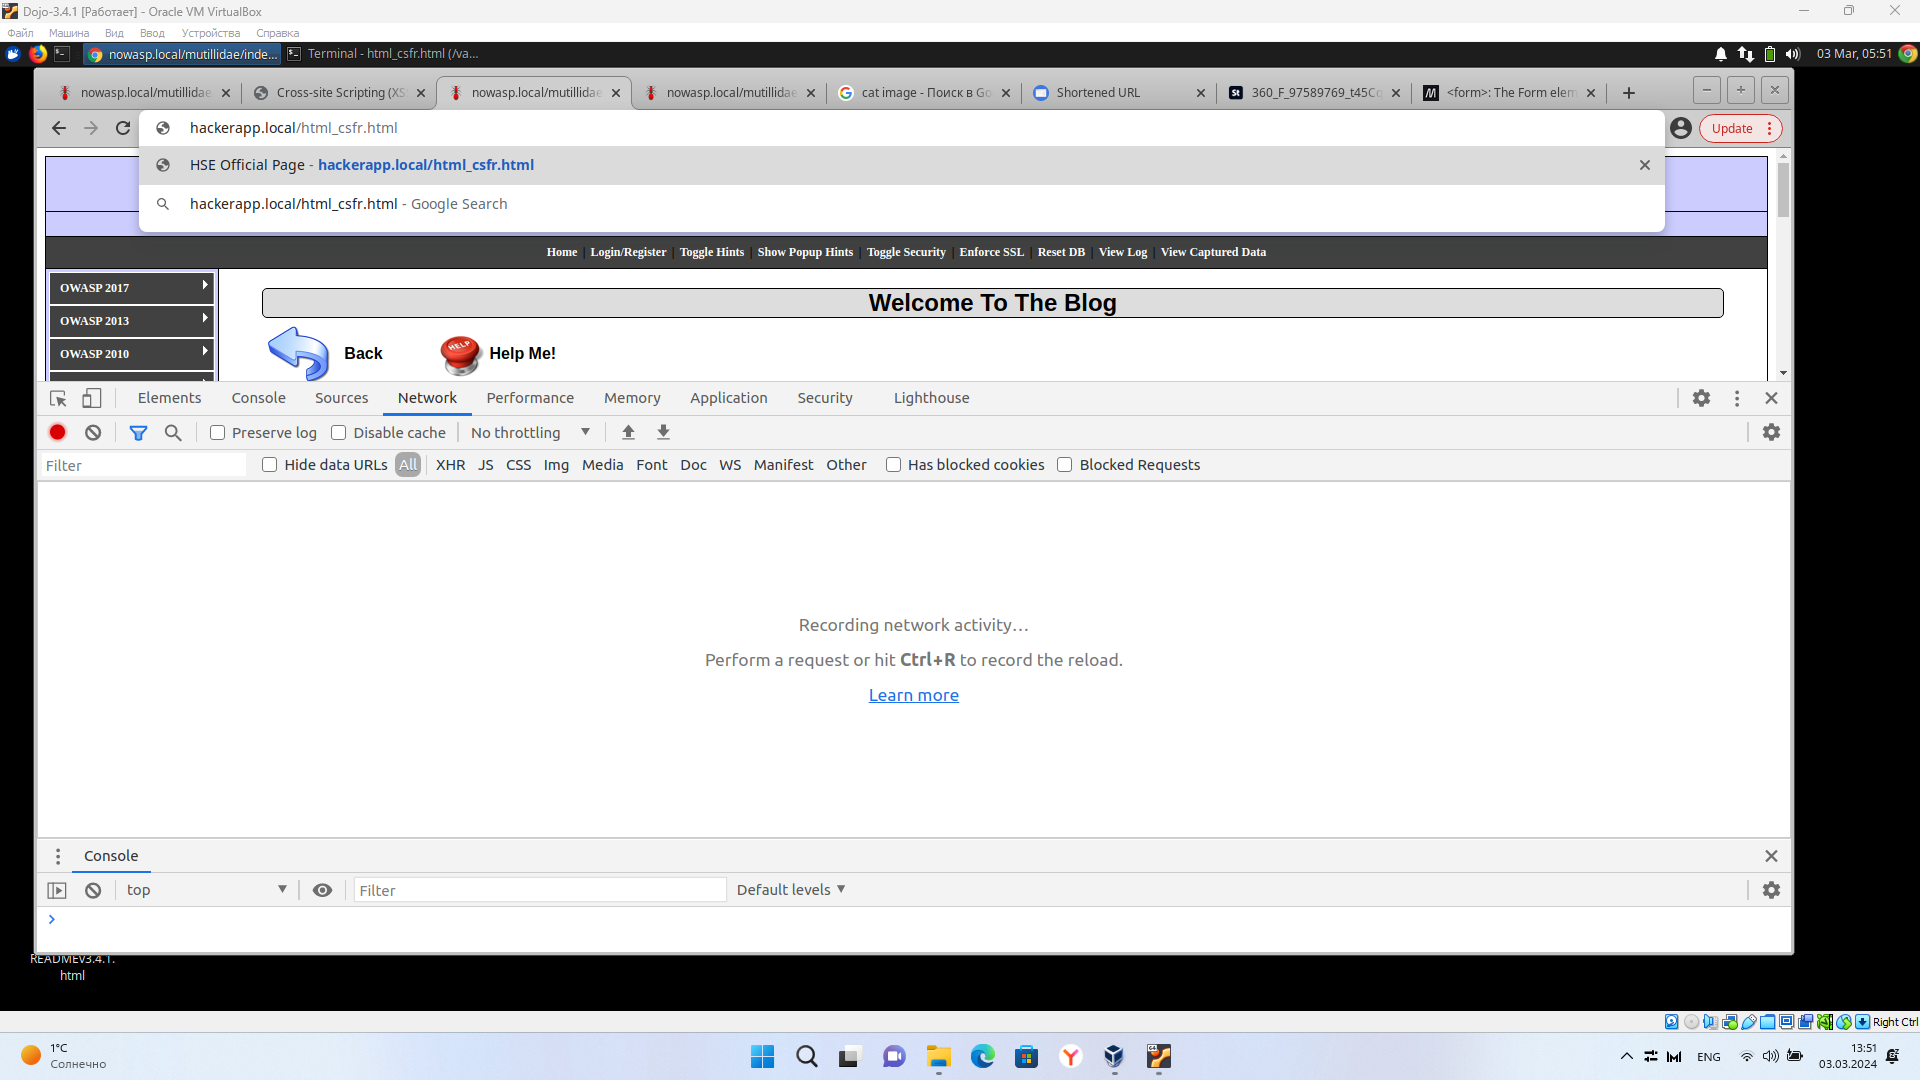
\includegraphics[width=\textwidth]{Screenshot_58}
    \caption{Видим, что браузер проставил cookie сессии и запрос выполнился успешно}
  \end{figure}

  Попробуем провести такую же атаку при помощи Ajax запроса:

  \begin{figure}[H]
    \centering
    \includegraphics[width=\textwidth]{Screenshot_72}
    \caption{Пишем скрипт для выполнения запроса}
  \end{figure}

  \begin{figure}[H]
    \centering
    \includegraphics[width=\textwidth]{Screenshot_73}
    \caption{Загружаем страницу со скриптом}
  \end{figure}

  \begin{figure}[H]
    \centering
    \includegraphics[width=\textwidth]{Screenshot_77}
    \caption{Видим в списке сетевых запросов запрос на добавление поста}
  \end{figure}

  \begin{figure}[H]
    \centering
    \includegraphics[width=\textwidth]{Screenshot_78}
    \caption{Бразер проставил cookie сессии}
  \end{figure}

  \begin{figure}[H]
    \centering
    \includegraphics[width=\textwidth]{Screenshot_79}
    \caption{Пост появился в списке}
  \end{figure}

  \subsection{Атака на dvwa.local}

  \subsubsection{Вход на атакуемый сайт}

  \begin{figure}[H]
    \centering
    \includegraphics[width=\textwidth]{Screenshot_84}
    \caption{Открываем сайт}
  \end{figure}

  \begin{figure}[H]
    \centering
    \includegraphics[width=\textwidth]{Screenshot_86}
    \caption{Вводим логин и пароль}
  \end{figure}

  \begin{figure}[H]
    \centering
    \includegraphics[width=\textwidth]{Screenshot_87}
    \caption{Сайт для атаки}
  \end{figure}

  \begin{figure}[H]
    \centering
    \includegraphics[width=\textwidth]{Screenshot_88}
    \caption{Устанавливаем уровень безопасности Low}
  \end{figure}

  \subsubsection{Анализ атакуемой страницы}

  \begin{figure}[H]
    \centering
    \includegraphics[width=\textwidth]{Screenshot_89}
    \caption{Открываем страницу для атаки}
  \end{figure}

  \begin{figure}[H]
    \centering
    \includegraphics[width=\textwidth]{Screenshot_90}
    \caption{Запускам анализ сетевых запросов}
  \end{figure}

  \begin{figure}[H]
    \centering
    \includegraphics[width=\textwidth]{Screenshot_91}
    \caption{Видим запрос на смену пароля}
  \end{figure}

  Этот запрос - GET запрос где новый пароль передается как query параметры

  \begin{figure}[H]
    \centering
    \includegraphics[width=\textwidth]{Screenshot_92}
    \caption{Cookie сессии}
  \end{figure}

  \begin{figure}[H]
    \centering
    \includegraphics[width=\textwidth]{Screenshot_93}
    \caption{Query параметры с новым паролем}
  \end{figure}

  \subsubsection{Выполняем атаку}

  \begin{figure}[H]
    \centering
    \includegraphics[width=\textwidth]{Screenshot_94}
    \caption{Создаем шаблон страницы злоумышленника}
  \end{figure}

  \begin{figure}[H]
    \centering
    \includegraphics[width=\textwidth]{Screenshot_95}
    \caption{Страница открывается с картинкой}
  \end{figure}

  \begin{figure}[H]
    \centering
    \includegraphics[width=\textwidth]{Screenshot_96}
    \caption{Скрываем картинку от пользователя, чтобы использовать img тег для атаки}
  \end{figure}

  \begin{figure}[H]
    \centering
    \includegraphics[width=\textwidth]{Screenshot_97}
    \caption{Картинка исчезла}
  \end{figure}

  \begin{figure}[H]
    \centering
    \includegraphics[width=\textwidth]{Screenshot_98}
    \caption{Указываем вместо src картинки подделанный запрос на смену пароля}
  \end{figure}

  \begin{figure}[H]
    \centering
    \includegraphics[width=\textwidth]{Screenshot_99}
    \caption{Переходим на страницу злоумышленника}
  \end{figure}

  \begin{figure}[H]
    \centering
    \includegraphics[width=\textwidth]{Screenshot_100}
    \caption{Запрс на смену пароля выполнился}
  \end{figure}

  \begin{figure}[H]
    \centering
    \includegraphics[width=\textwidth]{Screenshot_101}
    \caption{Проставим другой пароль}
  \end{figure}

  \begin{figure}[H]
    \centering
    \includegraphics[width=\textwidth]{Screenshot_102}
    \caption{Пробуем через другой браузер - запрос тоже прошел}
  \end{figure}

  \begin{figure}[H]
    \centering
    \includegraphics[width=\textwidth]{Screenshot_103}
    \caption{Cookie к этому get запросу были проставленны - атака выполнена}
  \end{figure}

  Здесь код ответа не 200, потому что далее происходит редирект на страницу смены пароля с сообщением об успехе.
  Далее для удобства снова используется атака на основе автоматической отправки html формы:

  \begin{figure}[H]
    \centering
    \includegraphics[width=\textwidth]{Screenshot_105}
    \caption{Вот об этой странице идет речь}
  \end{figure}

  \begin{figure}[H]
    \centering
    \includegraphics[width=\textwidth]{Screenshot_107}
    \caption{Проставим высокий уровень защиты}
  \end{figure}

  \begin{figure}[H]
    \centering
    \includegraphics[width=\textwidth]{Screenshot_108}
    \caption{Открываем страницу злоумышленника}
  \end{figure}

  \begin{figure}[H]
    \centering
    \includegraphics[width=\textwidth]{Screenshot_109}
    \caption{Запрос выполнился}
  \end{figure}

  \begin{figure}[H]
    \centering
    \includegraphics[width=\textwidth]{Screenshot_110}
    \caption{Cookie были проставлены, но пароль не поменялся}
  \end{figure}

  \begin{figure}[H]
    \centering
    \includegraphics[width=\textwidth]{Screenshot_111}
    \caption{Причина - отсутствие csfr токена}
  \end{figure}

  \begin{figure}[H]
    \centering
    \includegraphics[width=\textwidth]{Screenshot_112}
    \caption{Вилим этот токен в html разметки страницы}
  \end{figure}

\newpage
\section{Вывод}

В ходе данной работы были выполнениы csfr атаки при помощи cros-site запросов при помощи img тегов, отправки html форм и запуском скрытых ajax запросов

\end{document}

